% Options for packages loaded elsewhere
\PassOptionsToPackage{unicode}{hyperref}
\PassOptionsToPackage{hyphens}{url}
\PassOptionsToPackage{dvipsnames,svgnames,x11names}{xcolor}
%
\documentclass[
  letterpaper,
  DIV=11,
  numbers=noendperiod]{scrreprt}

\usepackage{amsmath,amssymb}
\usepackage{iftex}
\ifPDFTeX
  \usepackage[T1]{fontenc}
  \usepackage[utf8]{inputenc}
  \usepackage{textcomp} % provide euro and other symbols
\else % if luatex or xetex
  \usepackage{unicode-math}
  \defaultfontfeatures{Scale=MatchLowercase}
  \defaultfontfeatures[\rmfamily]{Ligatures=TeX,Scale=1}
\fi
\usepackage{lmodern}
\ifPDFTeX\else  
    % xetex/luatex font selection
\fi
% Use upquote if available, for straight quotes in verbatim environments
\IfFileExists{upquote.sty}{\usepackage{upquote}}{}
\IfFileExists{microtype.sty}{% use microtype if available
  \usepackage[]{microtype}
  \UseMicrotypeSet[protrusion]{basicmath} % disable protrusion for tt fonts
}{}
\makeatletter
\@ifundefined{KOMAClassName}{% if non-KOMA class
  \IfFileExists{parskip.sty}{%
    \usepackage{parskip}
  }{% else
    \setlength{\parindent}{0pt}
    \setlength{\parskip}{6pt plus 2pt minus 1pt}}
}{% if KOMA class
  \KOMAoptions{parskip=half}}
\makeatother
\usepackage{xcolor}
\setlength{\emergencystretch}{3em} % prevent overfull lines
\setcounter{secnumdepth}{5}
% Make \paragraph and \subparagraph free-standing
\makeatletter
\ifx\paragraph\undefined\else
  \let\oldparagraph\paragraph
  \renewcommand{\paragraph}{
    \@ifstar
      \xxxParagraphStar
      \xxxParagraphNoStar
  }
  \newcommand{\xxxParagraphStar}[1]{\oldparagraph*{#1}\mbox{}}
  \newcommand{\xxxParagraphNoStar}[1]{\oldparagraph{#1}\mbox{}}
\fi
\ifx\subparagraph\undefined\else
  \let\oldsubparagraph\subparagraph
  \renewcommand{\subparagraph}{
    \@ifstar
      \xxxSubParagraphStar
      \xxxSubParagraphNoStar
  }
  \newcommand{\xxxSubParagraphStar}[1]{\oldsubparagraph*{#1}\mbox{}}
  \newcommand{\xxxSubParagraphNoStar}[1]{\oldsubparagraph{#1}\mbox{}}
\fi
\makeatother


\providecommand{\tightlist}{%
  \setlength{\itemsep}{0pt}\setlength{\parskip}{0pt}}\usepackage{longtable,booktabs,array}
\usepackage{calc} % for calculating minipage widths
% Correct order of tables after \paragraph or \subparagraph
\usepackage{etoolbox}
\makeatletter
\patchcmd\longtable{\par}{\if@noskipsec\mbox{}\fi\par}{}{}
\makeatother
% Allow footnotes in longtable head/foot
\IfFileExists{footnotehyper.sty}{\usepackage{footnotehyper}}{\usepackage{footnote}}
\makesavenoteenv{longtable}
\usepackage{graphicx}
\makeatletter
\def\maxwidth{\ifdim\Gin@nat@width>\linewidth\linewidth\else\Gin@nat@width\fi}
\def\maxheight{\ifdim\Gin@nat@height>\textheight\textheight\else\Gin@nat@height\fi}
\makeatother
% Scale images if necessary, so that they will not overflow the page
% margins by default, and it is still possible to overwrite the defaults
% using explicit options in \includegraphics[width, height, ...]{}
\setkeys{Gin}{width=\maxwidth,height=\maxheight,keepaspectratio}
% Set default figure placement to htbp
\makeatletter
\def\fps@figure{htbp}
\makeatother
% definitions for citeproc citations
\NewDocumentCommand\citeproctext{}{}
\NewDocumentCommand\citeproc{mm}{%
  \begingroup\def\citeproctext{#2}\cite{#1}\endgroup}
\makeatletter
 % allow citations to break across lines
 \let\@cite@ofmt\@firstofone
 % avoid brackets around text for \cite:
 \def\@biblabel#1{}
 \def\@cite#1#2{{#1\if@tempswa , #2\fi}}
\makeatother
\newlength{\cslhangindent}
\setlength{\cslhangindent}{1.5em}
\newlength{\csllabelwidth}
\setlength{\csllabelwidth}{3em}
\newenvironment{CSLReferences}[2] % #1 hanging-indent, #2 entry-spacing
 {\begin{list}{}{%
  \setlength{\itemindent}{0pt}
  \setlength{\leftmargin}{0pt}
  \setlength{\parsep}{0pt}
  % turn on hanging indent if param 1 is 1
  \ifodd #1
   \setlength{\leftmargin}{\cslhangindent}
   \setlength{\itemindent}{-1\cslhangindent}
  \fi
  % set entry spacing
  \setlength{\itemsep}{#2\baselineskip}}}
 {\end{list}}
\usepackage{calc}
\newcommand{\CSLBlock}[1]{\hfill\break\parbox[t]{\linewidth}{\strut\ignorespaces#1\strut}}
\newcommand{\CSLLeftMargin}[1]{\parbox[t]{\csllabelwidth}{\strut#1\strut}}
\newcommand{\CSLRightInline}[1]{\parbox[t]{\linewidth - \csllabelwidth}{\strut#1\strut}}
\newcommand{\CSLIndent}[1]{\hspace{\cslhangindent}#1}

\KOMAoption{captions}{tableheading}
\makeatletter
\@ifpackageloaded{tcolorbox}{}{\usepackage[skins,breakable]{tcolorbox}}
\@ifpackageloaded{fontawesome5}{}{\usepackage{fontawesome5}}
\definecolor{quarto-callout-color}{HTML}{909090}
\definecolor{quarto-callout-note-color}{HTML}{0758E5}
\definecolor{quarto-callout-important-color}{HTML}{CC1914}
\definecolor{quarto-callout-warning-color}{HTML}{EB9113}
\definecolor{quarto-callout-tip-color}{HTML}{00A047}
\definecolor{quarto-callout-caution-color}{HTML}{FC5300}
\definecolor{quarto-callout-color-frame}{HTML}{acacac}
\definecolor{quarto-callout-note-color-frame}{HTML}{4582ec}
\definecolor{quarto-callout-important-color-frame}{HTML}{d9534f}
\definecolor{quarto-callout-warning-color-frame}{HTML}{f0ad4e}
\definecolor{quarto-callout-tip-color-frame}{HTML}{02b875}
\definecolor{quarto-callout-caution-color-frame}{HTML}{fd7e14}
\makeatother
\makeatletter
\@ifpackageloaded{bookmark}{}{\usepackage{bookmark}}
\makeatother
\makeatletter
\@ifpackageloaded{caption}{}{\usepackage{caption}}
\AtBeginDocument{%
\ifdefined\contentsname
  \renewcommand*\contentsname{Table of contents}
\else
  \newcommand\contentsname{Table of contents}
\fi
\ifdefined\listfigurename
  \renewcommand*\listfigurename{List of Figures}
\else
  \newcommand\listfigurename{List of Figures}
\fi
\ifdefined\listtablename
  \renewcommand*\listtablename{List of Tables}
\else
  \newcommand\listtablename{List of Tables}
\fi
\ifdefined\figurename
  \renewcommand*\figurename{Figure}
\else
  \newcommand\figurename{Figure}
\fi
\ifdefined\tablename
  \renewcommand*\tablename{Table}
\else
  \newcommand\tablename{Table}
\fi
}
\@ifpackageloaded{float}{}{\usepackage{float}}
\floatstyle{ruled}
\@ifundefined{c@chapter}{\newfloat{codelisting}{h}{lop}}{\newfloat{codelisting}{h}{lop}[chapter]}
\floatname{codelisting}{Listing}
\newcommand*\listoflistings{\listof{codelisting}{List of Listings}}
\makeatother
\makeatletter
\makeatother
\makeatletter
\@ifpackageloaded{caption}{}{\usepackage{caption}}
\@ifpackageloaded{subcaption}{}{\usepackage{subcaption}}
\makeatother
\newcounter{quartocalloutnteno}
\newcommand{\quartocalloutnte}[1]{\refstepcounter{quartocalloutnteno}\label{#1}}
\newcounter{quartocallouttipno}
\newcommand{\quartocallouttip}[1]{\refstepcounter{quartocallouttipno}\label{#1}}
\newcounter{quartocalloutimpno}
\newcommand{\quartocalloutimp}[1]{\refstepcounter{quartocalloutimpno}\label{#1}}

\ifLuaTeX
  \usepackage{selnolig}  % disable illegal ligatures
\fi
\usepackage{bookmark}

\IfFileExists{xurl.sty}{\usepackage{xurl}}{} % add URL line breaks if available
\urlstyle{same} % disable monospaced font for URLs
\hypersetup{
  pdftitle={The Regression Cookbook},
  pdfauthor={; Andy Tai; Ben Chen},
  colorlinks=true,
  linkcolor={blue},
  filecolor={Maroon},
  citecolor={Blue},
  urlcolor={Blue},
  pdfcreator={LaTeX via pandoc}}


\title{The Regression Cookbook}
\usepackage{etoolbox}
\makeatletter
\providecommand{\subtitle}[1]{% add subtitle to \maketitle
  \apptocmd{\@title}{\par {\large #1 \par}}{}{}
}
\makeatother
\subtitle{\textbf{Now with Machine Learning and Stats Flavours!}}
\author{G. Alexi Rodríguez-Arelis \and Andy Tai \and Ben Chen}
\date{2024-08-24}

\begin{document}
\maketitle
\begin{abstract}
This book aims to set a common ground between machine learning and
statistics regarding linear regression techniques, using \texttt{Python}
and \texttt{R}, under two perspectives: \textbf{inference} and
\textbf{prediction}.
\end{abstract}

\renewcommand*\contentsname{Table of contents}
{
\hypersetup{linkcolor=}
\setcounter{tocdepth}{2}
\tableofcontents
}

\bookmarksetup{startatroot}

\chapter*{Preface}\label{preface}
\addcontentsline{toc}{chapter}{Preface}

\markboth{Preface}{Preface}

\begin{quote}
\textbf{Let the regression cooking begin!}
\end{quote}

Data science is a field in which we become aware of the fascinating
overlap between \textbf{machine learning} and \textbf{statistics}. Many
data science students usually come across everyday machine learning and
statistics concepts or ideas that might only differ in names. For
instance, simple terms such as weights in \textbf{supervised learning}
(and their statistical counterpart as regression coefficients) might be
misleading for students starting their data science formation. On the
other hand, from an instructor's perspective in a data science program
that subsets its courses in machine learning in \texttt{Python} and
statistics in \texttt{R}, regression courses in \texttt{R} also demand
the inclusion of \texttt{Python}-related packages as alternative tools.
Furthermore, in a graduate program such as the
\href{https://masterdatascience.ubc.ca/}{Master of Data Science (MDS)}
at the University of British Columbia, this is especially critical for
students whose career plan leans towards the industry job market where
\texttt{Python} is more heavily used.

That said, we can state that data science is a \textbf{substantial
synergy} between machine learning and statistics. Nevertheless, many
gaps between both disciplines still need to be addressed. Thus, closing
these critical gaps is imperative in a domain with accelerated growth,
such as data science. In this regard, the
\href{https://ubc-mds.github.io/resources_pages/terminology/}{MDS
Stat-ML dictionary} has inspired us to write this textbook. It basically
consists of \textbf{common ground} between \textbf{foundational
supervised learning models} from machine learning and \textbf{regression
models} commonly used in statistics. We strive to explore \textbf{linear
modelling approaches} as a primary step while highlighting different
terminology found in both fields. Furthermore, this discussion is more
comprehensive than a simple conceptual exploration. Hence, the second
step is \textbf{hands-on practice} via the corresponding \texttt{Python}
packages for machine learning and \texttt{R} for statistics.

\begin{tcolorbox}[enhanced jigsaw, bottomrule=.15mm, breakable, colback=white, leftrule=.75mm, coltitle=black, rightrule=.15mm, bottomtitle=1mm, title={Fun fact!}, opacitybacktitle=0.6, toprule=.15mm, titlerule=0mm, arc=.35mm, colbacktitle=quarto-callout-warning-color!10!white, toptitle=1mm, colframe=quarto-callout-warning-color-frame, left=2mm, opacityback=0]

While thinking about possible names for this work, I was planning to
name it ``\emph{Machine Learning and Statistics: A Common Ground.}''
Nevertheless, it was quite plain and boring! That said, this whole
textbook idea sounded analogous to a \textbf{cookbook}\footnotemark{},
given its heavily applied focus.\\

\textbf{Hence, the cookbook name idea}!

\end{tcolorbox}

\footnotetext{Special thanks to \emph{Jonathan Graves}, who mentioned
the \textbf{cookbook} term when this textbook was conceptualized during
very early stages.}

\section*{About the authors}\label{about-the-authors}
\addcontentsline{toc}{section}{About the authors}

\markright{About the authors}

\subsection*{G. Alexi
Rodríguez-Arelis}\label{g.-alexi-rodruxedguez-arelis}
\addcontentsline{toc}{subsection}{G. Alexi Rodríguez-Arelis}

\begin{longtable}[]{@{}
  >{\raggedright\arraybackslash}p{(\columnwidth - 2\tabcolsep) * \real{0.5000}}
  >{\raggedright\arraybackslash}p{(\columnwidth - 2\tabcolsep) * \real{0.5000}}@{}}
\toprule\noalign{}
\endhead
\bottomrule\noalign{}
\endlastfoot
\begin{minipage}[t]{\linewidth}\raggedright
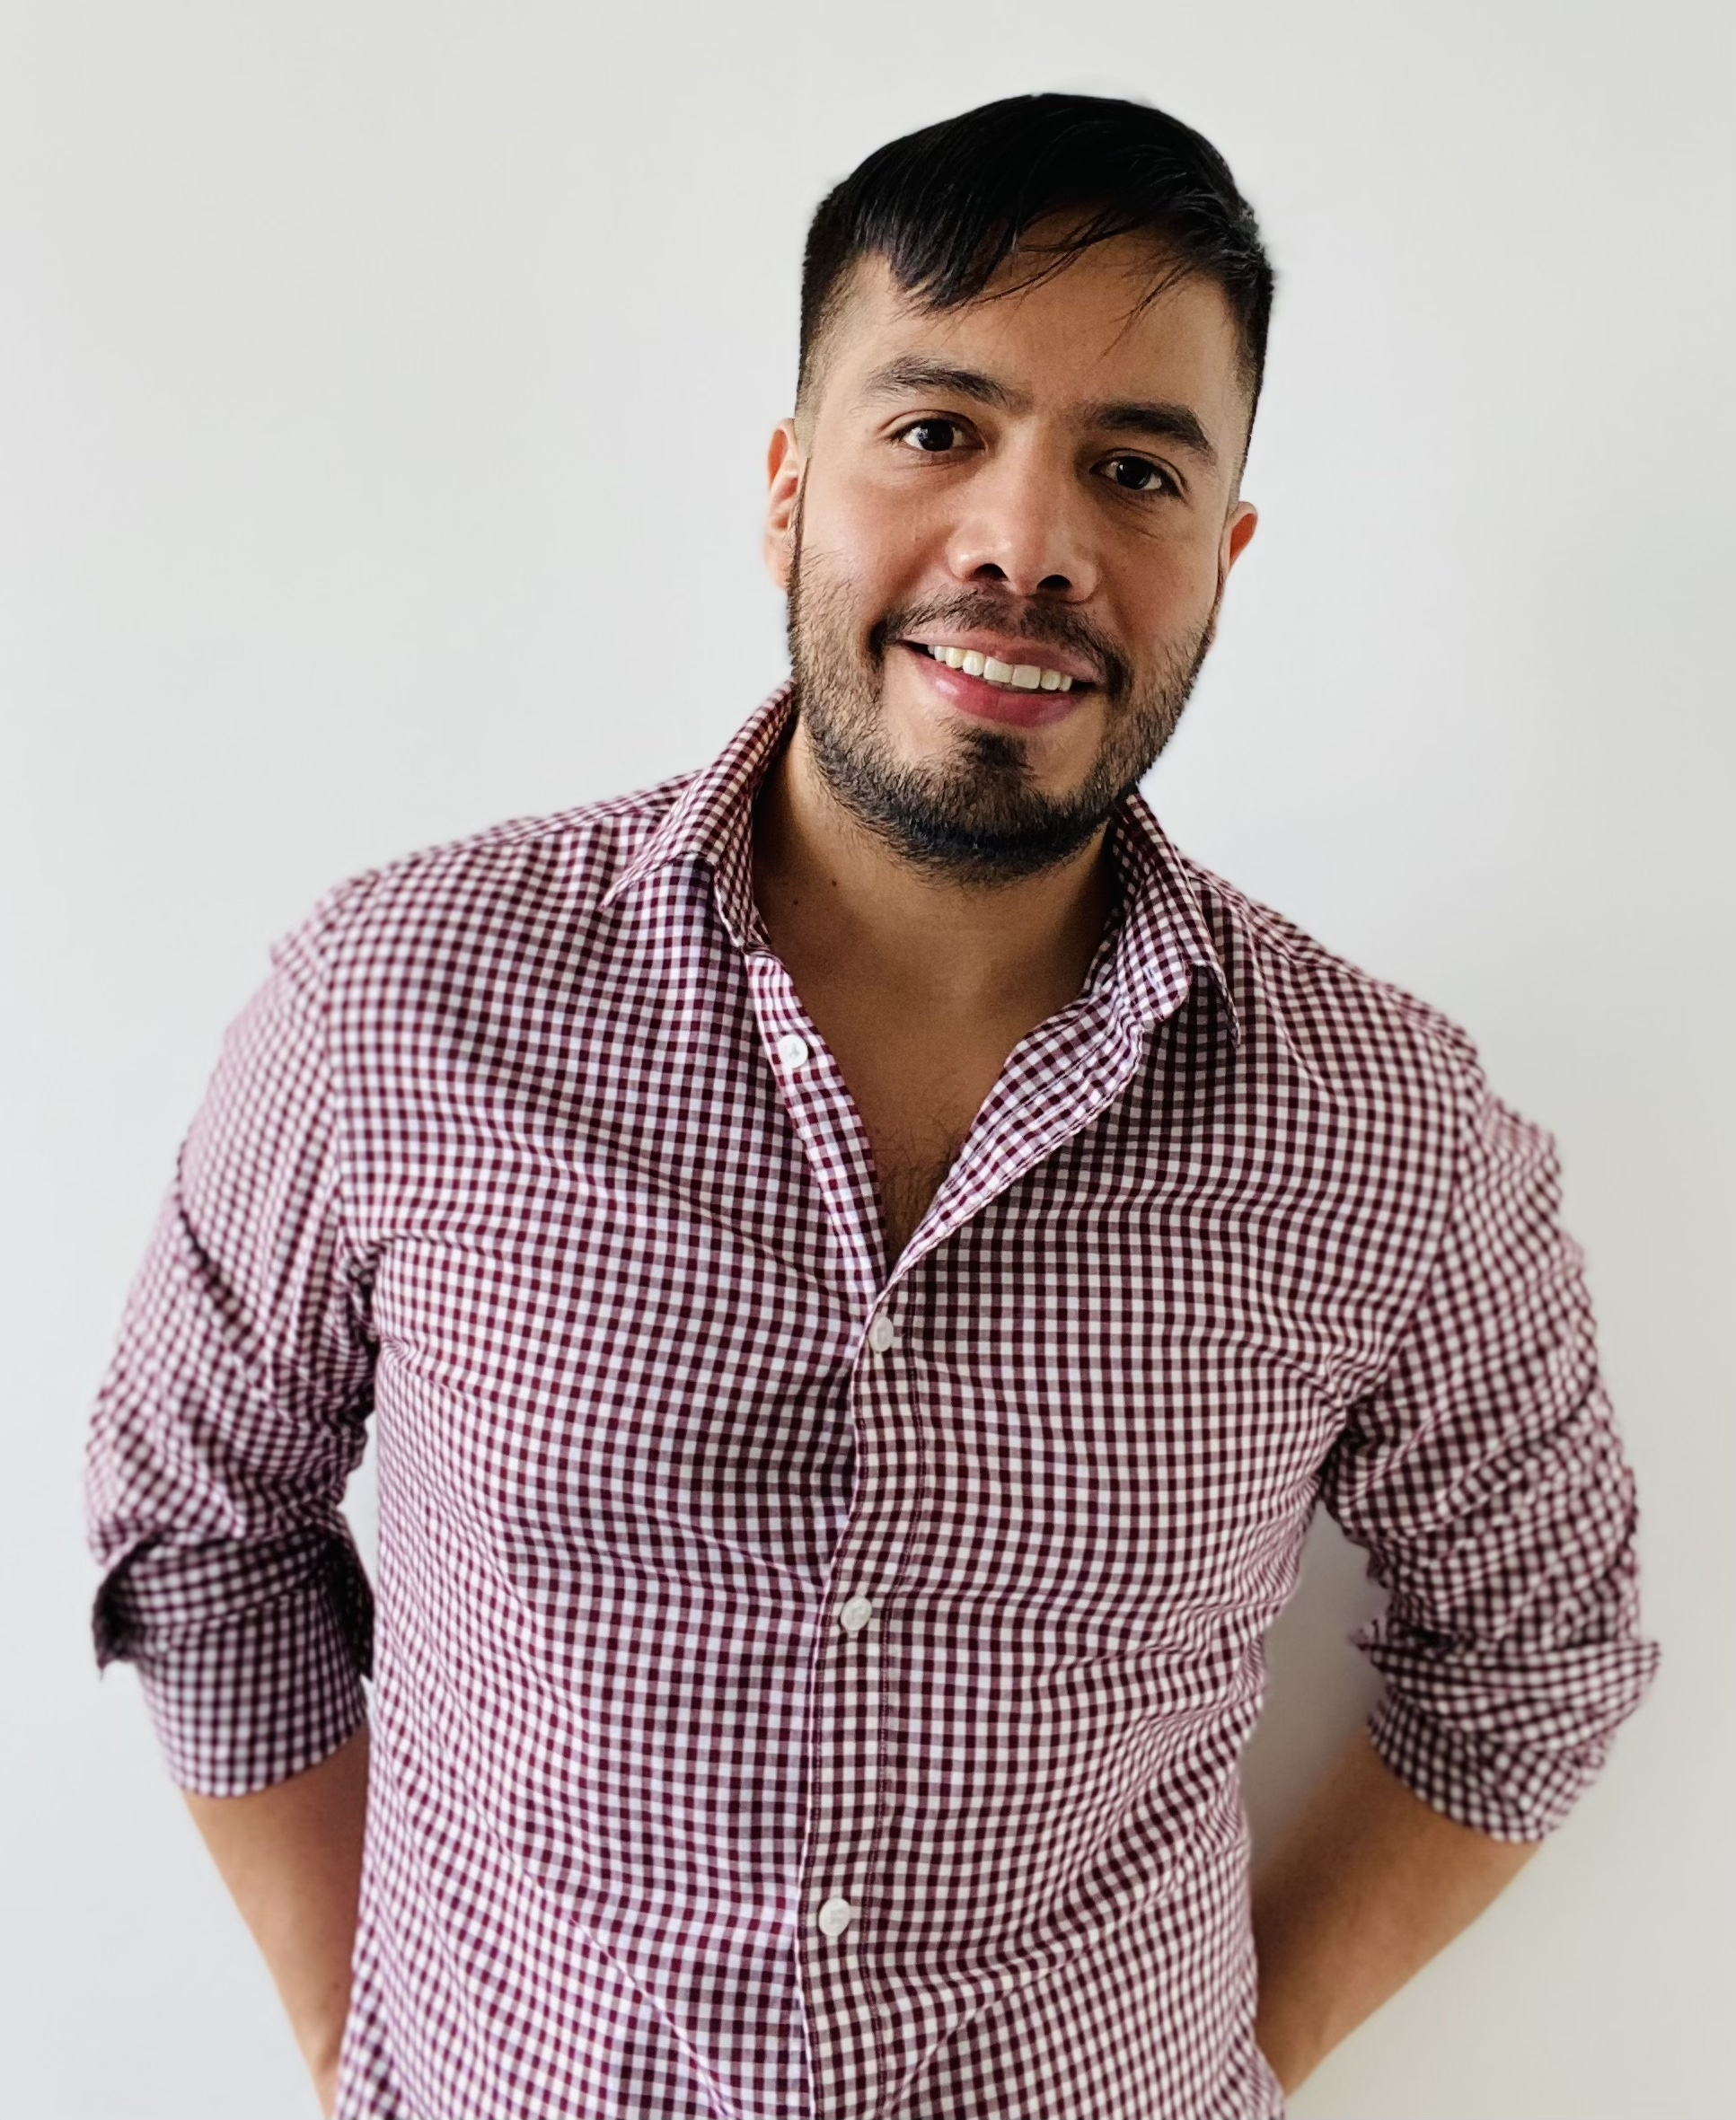
\includegraphics[width=3.64583in,height=\textheight]{img/photo-alexi.jpg}
\end{minipage} & \begin{minipage}[t]{\linewidth}\raggedright
\begin{quote}
I\textquotesingle m an Assistant Professor of Teaching in the Department
of Statistics and Master of Data Science at the University of British
Columbia. Throughout my academic and professional journey,
I\textquotesingle ve been involved in diverse fields, such as credit
risk management, statistical consulting, and data science teaching. My
doctoral research in statistics is primarily focused on computer
experiments that emulate scientific and engineering systems via Gaussian
stochastic processes (i.e., kriging regression). I\textquotesingle m
incredibly passionate about teaching regression topics while combining
statistical and machine learning contexts.
\end{quote}
\end{minipage} \\
\end{longtable}

\subsection*{Andy Tai}\label{andy-tai}
\addcontentsline{toc}{subsection}{Andy Tai}

\begin{longtable}[]{@{}
  >{\raggedright\arraybackslash}p{(\columnwidth - 2\tabcolsep) * \real{0.5000}}
  >{\raggedright\arraybackslash}p{(\columnwidth - 2\tabcolsep) * \real{0.5000}}@{}}
\toprule\noalign{}
\endhead
\bottomrule\noalign{}
\endlastfoot
\begin{minipage}[t]{\linewidth}\raggedright
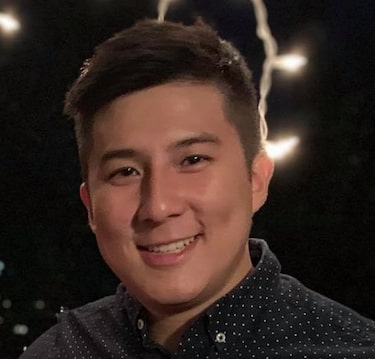
\includegraphics[width=3.64583in,height=\textheight]{img/photo-andy.jpg}
\end{minipage} & \begin{minipage}[t]{\linewidth}\raggedright
\begin{quote}
I\textquotesingle m a Postdoctoral Teaching and Learning Fellow in the
Department of Statistics and Master of Data Science at the University of
British Columbia. Throughout my academic and professional journey,
I\textquotesingle ve been involved in diverse fields, such as addiction
psychiatry, machine learning, and data science teaching. My doctoral
research in neuroscience primarily focused on using machine learning to
predict the risk of fatal overdose. I am interested in leveraging data
science and machine learning to solve complex problems, and I strive to
inspire others to explore the vast potential of these fields.
\end{quote}
\end{minipage} \\
\end{longtable}

\subsection*{Ben Chen}\label{ben-chen}
\addcontentsline{toc}{subsection}{Ben Chen}

\section*{License}\label{license}
\addcontentsline{toc}{section}{License}

\markright{License}

This work is licensed under a Creative Commons
Attribution-NonCommercial-ShareAlike 4.0 International License.

\bookmarksetup{startatroot}

\chapter*{Audience and Scope}\label{audience-and-scope}
\addcontentsline{toc}{chapter}{Audience and Scope}

\markboth{Audience and Scope}{Audience and Scope}

This book mainly focuses on \textbf{regression analysis} and its
\textbf{supervised learning} counterpart. Thus, it is not introductory
statistics and machine learning material. Also, some coding background
on \texttt{R} (R Core Team 2024) and/or \texttt{Python} (Van Rossum and
Drake 2009) is recommended. That said, the following topics are
suggested as \textbf{fundamental reviews}:

\begin{itemize}
\tightlist
\item
  \textbf{Mutivariable differential calculus and linear algebra.}
  Certain sections of each chapter pertain to modelling estimation.
  Therefore, topics such as \emph{partial derivatives} and \emph{matrix
  algebra} are a great asset. You can find helpful learning resources on
  the
  \href{https://ubc-mds.github.io/resources_pages/learning_resources/}{MDS
  webpage}.
\item
  \textbf{Basic \texttt{Python} programming.} When necessary,
  \texttt{Python} \href{https://pypi.org/project/pandas/}{\{pandas\}}
  (The Pandas Development Team 2024) library will be used to perform
  \emph{data wrangling}. The MDS course
  \href{https://github.com/UBC-MDS/DSCI_511_prog-dsci}{DSCI 511
  (Programming for Data Science)} is an ideal example of a quick review.
\end{itemize}

\begin{figure}[H]

{\centering 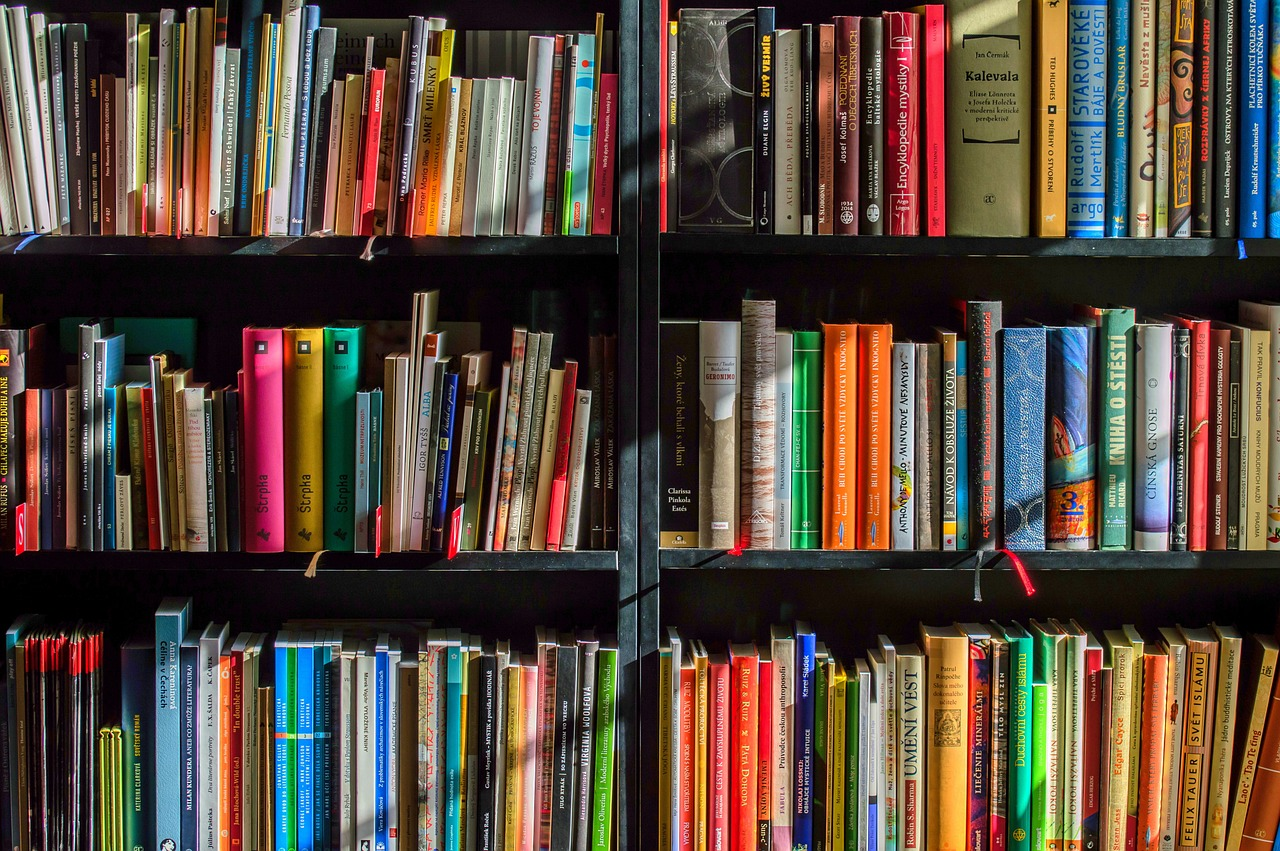
\includegraphics[width=5.20833in,height=\textheight]{book/img/books.jpg}

}

\caption{Image by
\href{https://pixabay.com/users/luboshouska-198496/}{\emph{Lubos
Houska}} via
\href{https://pixabay.com/photos/books-bookstore-book-reading-1204029/}{\emph{Pixabay}}.}

\end{figure}%

\begin{itemize}
\tightlist
\item
  \textbf{Basic \texttt{R} programming.} Knowledge of \emph{data
  wrangling and plotting} through \texttt{R}
  \href{https://www.tidyverse.org}{\{tidyverse\}} (Wickham et al. 2019)
  is recommended for hands-on practice via the cases provided in each
  one of the chapters of this book. The MDS courses
  \href{https://github.com/UBC-MDS/DSCI_523_r-prog}{DSCI 523
  (Programming for Data Manipulation)} and
  \href{https://github.com/UBC-MDS/DSCI_531_viz-1}{DSCI 531 (Data
  Visualization I)} are ideal examples of a quick review.
\item
  \textbf{Foundations of probability and basic distributional
  knowledge.} The reader should be familiar with elemental
  \emph{discrete and continuous distributions} since they are a vital
  component of any given regression or supervised learning model. The
  MDS course
  \href{https://ubc-mds.github.io/course-descriptions/DSCI_551_eda-dsci/}{DSCI
  551 (Descriptive Statistics and Probability for Data Science)} is an
  ideal example of a quick review.
\item
  \textbf{Foundations of frequentist statistical inference.} One of the
  data science paradigms to be covered in this book is \emph{statistical
  inference}, i.e., identifying relationships between different
  variables in a given \emph{population or system} of interest via a
  \emph{sampled dataset}. I only aim to cover a frequentist approach
  using inferential tools such as \emph{parameter estimation},
  \emph{hypothesis testing}, and \emph{confidence intervals}. The MDS
  course \href{https://github.com/UBC-MDS/DSCI_552_stat-inf-1}{DSCI 552
  (Statistical Inference and Computation I)} is an ideal example of a
  quick review.
\item
  \textbf{Foundations of supervised learning.} The second data science
  paradigm to be covered pertains to \emph{prediction}, which is core in
  machine learning. The reader should be familiar with basic
  terminology, such as \emph{training and testing data},
  \emph{overfitting}, \emph{underfitting}, \emph{cross-validation}, etc.
  The MDS course
  \href{https://github.com/UBC-MDS/DSCI_571_sup-learn-1}{DSCI 571
  (Machine Learning I)} provides these foundations.
\item
  \textbf{Foundations of feature and model selection.} This prerequisite
  also relates to machine learning and its corresponding prediction
  paradigm. Basic knowledge of \emph{prediction accuracy} and
  \emph{variable selection tools} is recommended. The MDS course
  \href{https://github.com/UBC-MDS/DSCI_573_feat-model-select}{DSCI 573
  (Feature and Model Selection)} is an ideal example of a quick review.
\end{itemize}

\begin{tcolorbox}[enhanced jigsaw, bottomrule=.15mm, breakable, colback=white, leftrule=.75mm, coltitle=black, rightrule=.15mm, bottomtitle=1mm, title={A further remark on probability and statistical inference}, opacitybacktitle=0.6, toprule=.15mm, titlerule=0mm, arc=.35mm, colbacktitle=quarto-callout-note-color!10!white, toptitle=1mm, colframe=quarto-callout-note-color-frame, left=2mm, opacityback=0]

In case the reader is not 100\% familiar with probabilistic and
inferential topics, as discussed above, we will provide a fundamental
refresher in Chapter~\ref{sec-stats-review} with crucial points that are
needed to follow along the \textbf{statistical way} each one of the
chapters is delivered (more specifically for \textbf{modelling
estimation/training} matters!).\\

Furthermore, this refresher will be integrated into \textbf{the three
big pillars} that will be fully expanded in this book, more concretely
in Chapter~\ref{sec-intro}: a \textbf{data science workflow}, the right
\textbf{workflow flavour} (\textbf{inferential} or \textbf{predictive}),
and a \textbf{regression toolbox}.

\end{tcolorbox}

\bookmarksetup{startatroot}

\chapter{Getting Ready for Regression Cooking!}\label{sec-intro}

It is time to prepare for all the different regression techniques we
will check beginning Chapter~\ref{sec-ols}. That said, there is a strong
message we want to convey across all this work:

\begin{quote}
\textbf{Different modelling estimation techniques in regression analysis
can be smoothly grasped when we develop a fair probabilistic and
inferential intuition on our populations or systems of interest.}
\end{quote}

The above statement has a fundamental statistical foundation on how data
is generated and can be modelled via different regression approaches.
More details on the concepts and ideas associated with this foundation
will be delivered in Chapter~\ref{sec-stats-review}. Hence, before
reviewing these statistical concepts and ideas, this chapter will
elaborate on the three big pillars we previously pointed out in
\textbf{Audience and Scope}:

\begin{enumerate}
\def\labelenumi{\arabic{enumi}.}
\tightlist
\item
  The use of an ordered \textbf{data science workflow} in
  Section~\ref{sec-ds-workflow},
\item
  choosing the proper workflow flavour according to either an
  \textbf{inferential} or \textbf{predictive} paradigm as shown in
  Figure~\ref{fig-ds-workflow}, and
\item
  the correct use of an \textbf{appropriate regression model} based on
  the response or outcome of interest as shown in the mind map from
  Section~\ref{sec-regression-mindmap} (analogous to a
  \textbf{regression toolbox}).
\end{enumerate}

\begin{figure}[H]

{\centering 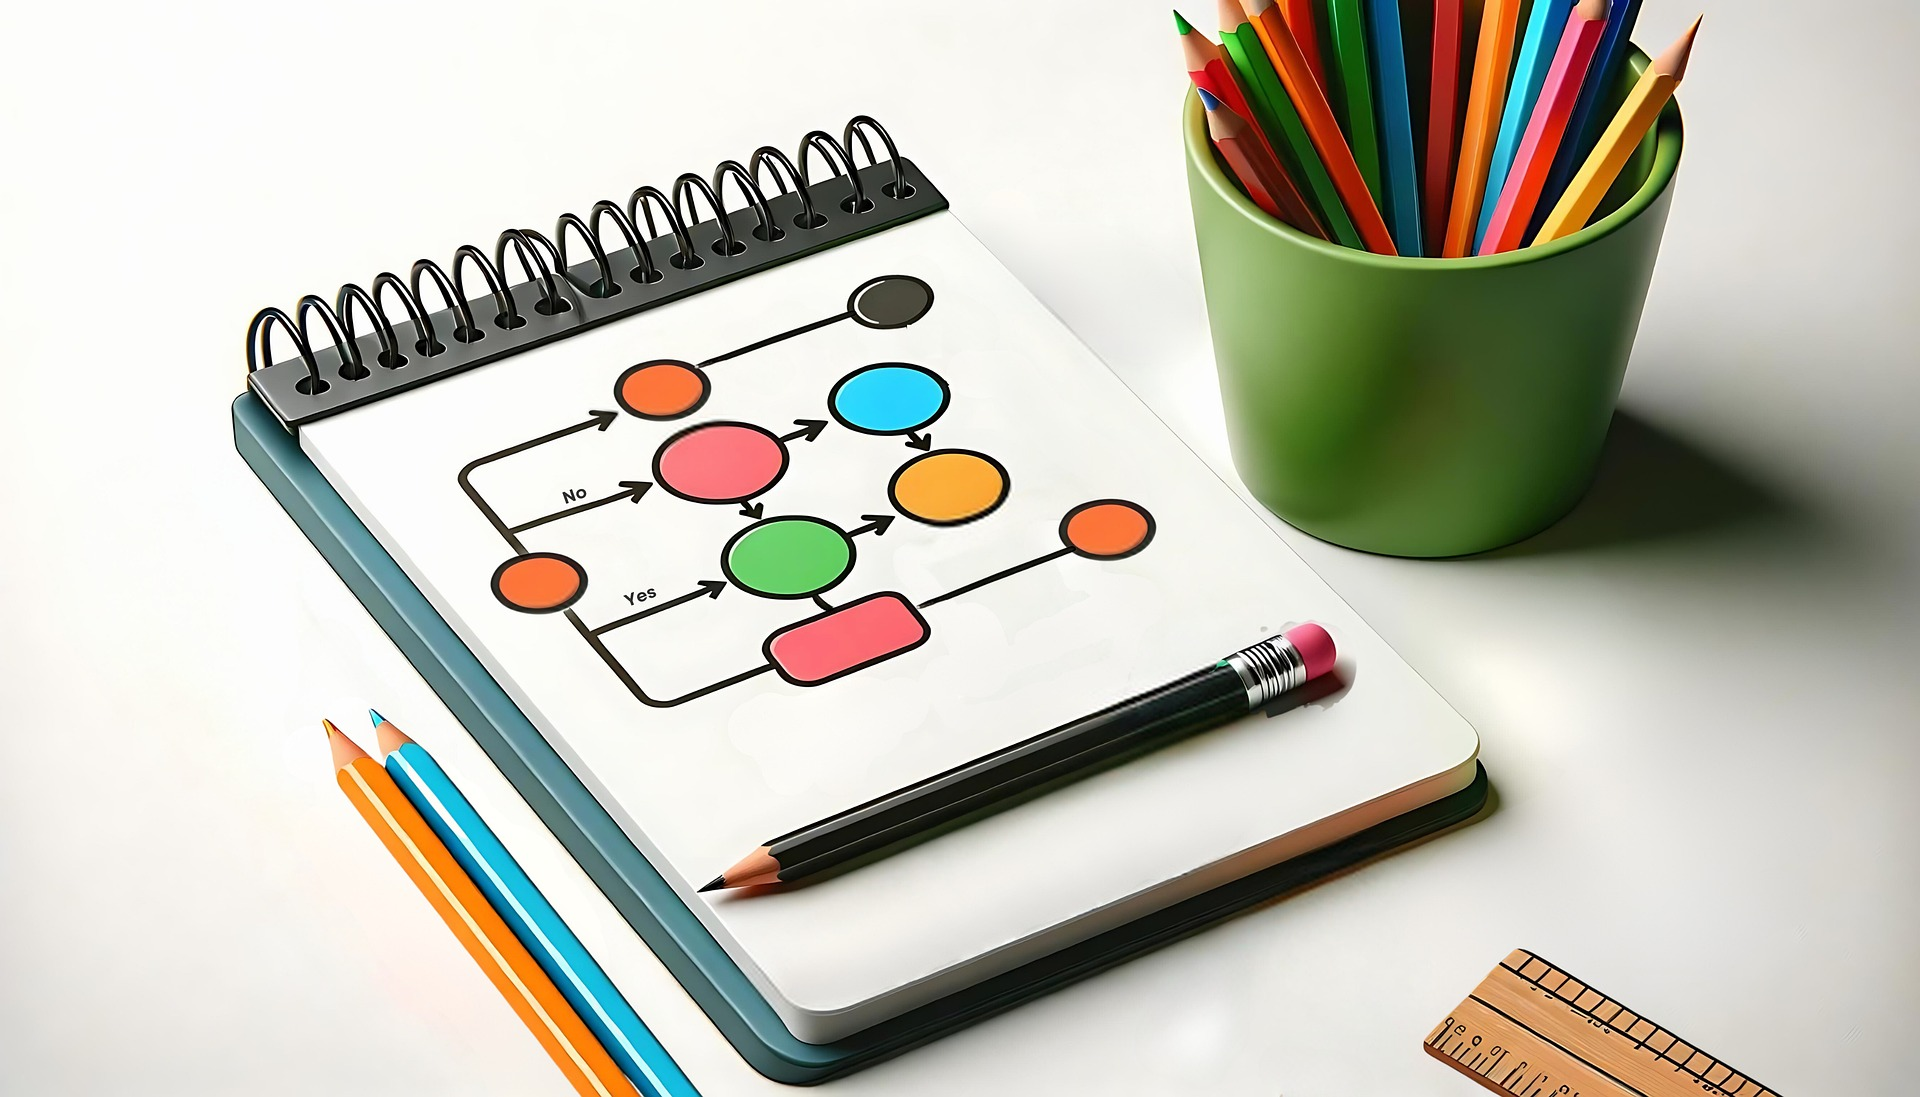
\includegraphics[width=5.20833in,height=\textheight]{book/img/flowchart.png}

}

\caption{Image by
\href{https://pixabay.com/users/lucasjisrael-43158173/}{\emph{Lucas
Israel}} via
\href{https://pixabay.com/illustrations/flowchart-diagram-sketch-notepad-8860311/}{\emph{Pixabay}}.}

\end{figure}%

\begin{tcolorbox}[enhanced jigsaw, bottomrule=.15mm, breakable, colback=white, leftrule=.75mm, coltitle=black, rightrule=.15mm, bottomtitle=1mm, title={The Rationale Behind the Three Pillars}, opacitybacktitle=0.6, toprule=.15mm, titlerule=0mm, arc=.35mm, colbacktitle=quarto-callout-tip-color!10!white, toptitle=1mm, colframe=quarto-callout-tip-color-frame, left=2mm, opacityback=0]

Each data science-related problem that uses regression analysis might
have distinctive characteristics considering inferential (statistics!)
or predictive (machine learning!) inquiries. Specific problems would
implicate using outcomes (or responses) related to survival times (e.g.,
the time until one particular equipment of a given brand fails),
categories (e.g., a preferred musical genre in the Canadian young
population), counts (e.g., how many customers we would expect on a
regular Monday morning in the branches of a major national bank), etc.
Moreover, under this regression context, our analyses would be expanded
to explore and assess how our outcome of interest is related to a
further set of variables (the so-called features!). For instance,
following up with the categorical outcome of the preferred musical genre
in the Canadian young population, we might analyze how particular age
groups prefer certain genres over others or even how preferred genres
compare each other across different Canadian provinces in this young
population. \textbf{The sky is the limit here!}\\

Therefore, we might be tempted to say that each regression problem
should have its own workflow, given that the regression model to use
would implicate particular analysis phases. \textbf{However, it turns
out that is not the case to a certain extent}, and we have a regression
workflow in Figure~\ref{fig-ds-workflow} to support this bold statement
as a proof of concept for thirteen different regression models (i.e,
thirteen chapters in this book aside from the probability and statistics
review). The workflow aims to homogenize our data analyses and make our
modelling process more transparent and smoother. We can adequately
deliver concluding insights as data storytelling while addressing our
initial main inquiries. Of course, when depicting the workflow as a
flowchart, there will be decision points that will turn it into
\textbf{inferential} or \textbf{predictive} (the second pillar).
Finally, where does the third pillar come into play in this workflow?
This pillar is contained in the \textbf{data modelling stage}, where the
mind map from Figure~\ref{fig-regression-mindmap} will come in handy.

\end{tcolorbox}

Moving along, let us establish a convention on the use of admonitions
beginning Section~\ref{sec-ml-stats-dictionary} in this textbook:

Definition

A formal statistical and/or machine learning definition. This admonition
aims to untangle the significant amount of jargon and concepts that both
fields have. Furthermore, alternative terminology will be brought up
when necessary to indicate the same definition across both fields.

\phantomsection\label{headsup1}
Heads-up!

An idea (or ideas!) of key relevance for any given modelling approach,
specific workflow stage or data science-related terminology. This
admonition also extends to crucial statistical or machine learning
topics that the reader would be interested in exploring more in-depth.

Tip

An idea (or ideas!) that might be slightly out of the scope of the topic
any specific section is discussing. Still, I will provide significant
insights on the matter along with further literature references to look
for.

See \hyperref[headsup1]{Heads-up}.

The core idea of the above admonition arrangement is to allow the reader
to discern between ideas or concepts that are key to grasp from those
whose understanding might not be highly essential (but still interesting
to check out in further literature!). Before jumping into our three
pillars in sections Section~\ref{sec-ds-workflow} and
Section~\ref{sec-regression-mindmap}, let us elaborate on an additional
resource related to setting a \textbf{common ground} between
\textbf{machine learning} and \textbf{statistics}.

\section{The ML-Stats Dictionary}\label{sec-ml-stats-dictionary}

Machine learning and statistics usually overlap across many subjects,
and regression modelling is no exception. Topics we teach in an utterly
regression-based course, under a purely statistical framework, also
appear in machine learning-based courses such as fundamental supervised
learning, but often with different terminology. On this basis, the
Master of Data Science (MDS) program at the University of British
Columbia (UBC) provides the
\href{https://ubc-mds.github.io/resources_pages/terminology/}{MDS
Stat-ML dictionary} (Gelbart 2017) under the following premises:

\begin{quote}
\emph{This document is intended to help students navigate the large
amount of jargon, terminology, and acronyms encountered in the MDS
program and beyond.}
\end{quote}

\begin{quote}
\emph{This section covers terms that have different meanings in
different contexts, specifically statistics vs.~machine learning (ML).}
\end{quote}

Indeed, both disciplines have a tremendous amount of jargon and
terminology. Furthermore, as previously emphasized in the
\textbf{Preface}, machine learning and statistics construct a
\textbf{substantial synergy} reflected in data science. Even with this,
people in both fields could encounter miscommunication issues when
working together. This should not happen if we build solid bridges
between both disciplines. Therefore, the above admonition in
\textbf{?@imp-example} for a \textbf{definition} will pave the way to a
complimentary resource called the \textbf{ML-Stats dictionary}
(\emph{ML} stands for \emph{Machine Learning}). This comprehensive
\textbf{ML-Stats dictionary} is imperative, and our textbook offers a
perfect opportunity to build this resource. Primarily, this dictionary
will clarify any potential confusion between statistics and machine
learning regarding terminology within supervised learning and regression
analysis contexts.

\begin{tcolorbox}[enhanced jigsaw, bottomrule=.15mm, breakable, colback=white, leftrule=.75mm, coltitle=black, rightrule=.15mm, bottomtitle=1mm, title=\textcolor{quarto-callout-note-color}{\faInfo}\hspace{0.5em}{Note \ref*{nte-term-highlight}: Heads-up on terminology highlights!}, opacitybacktitle=0.6, toprule=.15mm, titlerule=0mm, arc=.35mm, colbacktitle=quarto-callout-note-color!10!white, toptitle=1mm, colframe=quarto-callout-note-color-frame, left=2mm, opacityback=0]

\quartocalloutnte{nte-term-highlight} 

Following the spirit of the \textbf{ML-Stats dictionary}, throughout the
book, all \textcolor{blue}{statistical} terms will be highlighted in
\textcolor{blue}{blue} whereas the \textcolor{magenta}{machine learning}
terms will be highlighted in \textcolor{magenta}{magenta}. This colour
scheme strives to combine this terminology so we can switch from one
field to another in an easier way. With practice and time, we should be
able to jump back and forth when using these concepts.

\end{tcolorbox}

Finally, Appendix~\ref{sec-dictionary} will be the section in this book
where the reader can find all those \textcolor{blue}{statistical} and
\textcolor{magenta}{machine learning-related} terms in alphabetical
order. Notable terms (either statistical or machine learning-related)
will include an admonition identifying which terms (again, either
statistical or machine learning-related) are \textbf{equivalent}
(\textbf{or NOT equivalent if that is the case}). Take as an example the
statistical term \textcolor{blue}{dependent variable}:

\begin{quote}
In supervised learning, it is the main variable of interest we are
trying to \textbf{learn} or \textbf{predict}, or equivalently, the
variable we are trying \textbf{explain} in a statistical inference
framework.
\end{quote}

Then, the above definition will be followed by this admonition:

\begin{tcolorbox}[enhanced jigsaw, bottomrule=.15mm, breakable, colback=white, leftrule=.75mm, coltitle=black, rightrule=.15mm, bottomtitle=1mm, title=\textcolor{quarto-callout-warning-color}{\faExclamationTriangle}\hspace{0.5em}{Equivalent to:}, opacitybacktitle=0.6, toprule=.15mm, titlerule=0mm, arc=.35mm, colbacktitle=quarto-callout-warning-color!10!white, toptitle=1mm, colframe=quarto-callout-warning-color-frame, left=2mm, opacityback=0]

\textcolor{blue}{Response}, \textcolor{magenta}{outcome},
\textcolor{magenta}{output} or \textcolor{magenta}{target}.

\end{tcolorbox}

Above, we have identified four equivalent terms for the term
\textcolor{blue}{dependent variable}. Furthermore, according to our
already defined colour scheme, these terms can be
\textcolor{blue}{statistical} or
\textcolor{magenta}{machine learning-related}. Finally, note we will
start using this colour scheme in Chapter~\ref{sec-stats-review}.

\begin{tcolorbox}[enhanced jigsaw, bottomrule=.15mm, breakable, colback=white, leftrule=.75mm, coltitle=black, rightrule=.15mm, bottomtitle=1mm, title=\textcolor{quarto-callout-note-color}{\faInfo}\hspace{0.5em}{Note \ref*{nte-use-terminology}: Heads-up on the use of terminology!}, opacitybacktitle=0.6, toprule=.15mm, titlerule=0mm, arc=.35mm, colbacktitle=quarto-callout-note-color!10!white, toptitle=1mm, colframe=quarto-callout-note-color-frame, left=2mm, opacityback=0]

\quartocalloutnte{nte-use-terminology} 

Throughout this book, we will interchangeably use specific terms when
explaining the different regression approaches in each chapter. Whenever
confusion arises about using these interchangeable terms, it is highly
recommended to consult their definitions and equivalences (or
non-equivalences) in Appendix~\ref{sec-dictionary}.

\end{tcolorbox}

Now, let us proceed to explaining the three pillars on which this
textbook is built upon: a \textbf{data science workflow}, the right
\textbf{workflow flavour} (\textbf{inferential} or \textbf{predictive}),
and a \textbf{regression toolbox}.

\section{The Data Science Workflow}\label{sec-ds-workflow}

Understanding the data science workflow is essential for mastering
regression analysis. This workflow serves as a blueprint that guides us
through each stage of our analysis, ensuring that we apply a systematic
approach to solving our inquiries in a reproducible way. Each of the
three pillars of this textbook---data science workflow, the right
workflow flavor (inferential or predictive), and a regression
toolbox---are deeply interconnected. Regardless of the regression model
we explore, this general workflow provides a consistent framework that
helps us navigate our data analysis with clarity and purpose. As shown
in Figure~\ref{fig-ds-workflow}, the data science workflow is composed
of the following stages (each of which will be discussed in more detail
in subsequent subsections):

\begin{enumerate}
\def\labelenumi{\arabic{enumi}.}
\tightlist
\item
  \textbf{Study design:} Define the research question, objectives, and
  variables of interest to ensure the analysis is purpose-driven and
  aligned with the problem at hand.
\item
  \textbf{Data collection and wrangling:} Gather and clean data,
  addressing issues such as missing values, outliers, and
  inconsistencies to transform it into a usable format.
\item
  \textbf{Exploratory data analysis:} Explore the data through
  statistical summaries and visualizations to identify patterns, trends,
  and potential anomalies.
\item
  \textbf{Data modelling:} Apply statistical or machine learning models
  to uncover relationships between variables or make predictions based
  on the data.
\item
  \textbf{Estimation:} Calculate model parameters to quantify
  relationships between variables and assess the accuracy and
  reliability of the model.
\item
  \textbf{Goodness of fit:} Evaluate the model's performance using
  metrics and diagnostic checks to determine how well it explains the
  data.
\item
  \textbf{Results:} Interpret the model's outputs to derive meaningful
  insights and provide answers to the original research question.
\item
  \textbf{Storytelling} Communicate the findings through a clear,
  engaging narrative that is accessible to a non-technical audience.
\end{enumerate}

By adhering to this workflow, we ensure that our regression analyses are
not only systematic and thorough but also capable of producing results
that are meaningful within the context of the problem we aim to solve.

\begin{tcolorbox}[enhanced jigsaw, bottomrule=.15mm, breakable, colback=white, leftrule=.75mm, coltitle=black, rightrule=.15mm, bottomtitle=1mm, title=\textcolor{quarto-callout-note-color}{\faInfo}\hspace{0.5em}{The Importance of a Formal Structure in Regression Analysis}, opacitybacktitle=0.6, toprule=.15mm, titlerule=0mm, arc=.35mm, colbacktitle=quarto-callout-note-color!10!white, toptitle=1mm, colframe=quarto-callout-note-color-frame, left=2mm, opacityback=0]

From the earliest stages of learning data analysis, understanding the
importance of a structured workflow is crucial. If we do not adhere to a
predefined workflow, we risk misinterpreting the data, leading to
incorrect conclusions that fail to address the core questions of our
analysis. Such missteps can result in outcomes that are not only
meaningless but potentially misleading when taken out of the problem's
context. Therefore, it is essential for aspiring data scientists to
internalize this workflow from the very beginning of their education. A
systematic approach ensures that each stage of the analysis is conducted
with precision, ultimately producing reliable and contextually relevant
results.

\end{tcolorbox}

\begin{figure}

\centering{

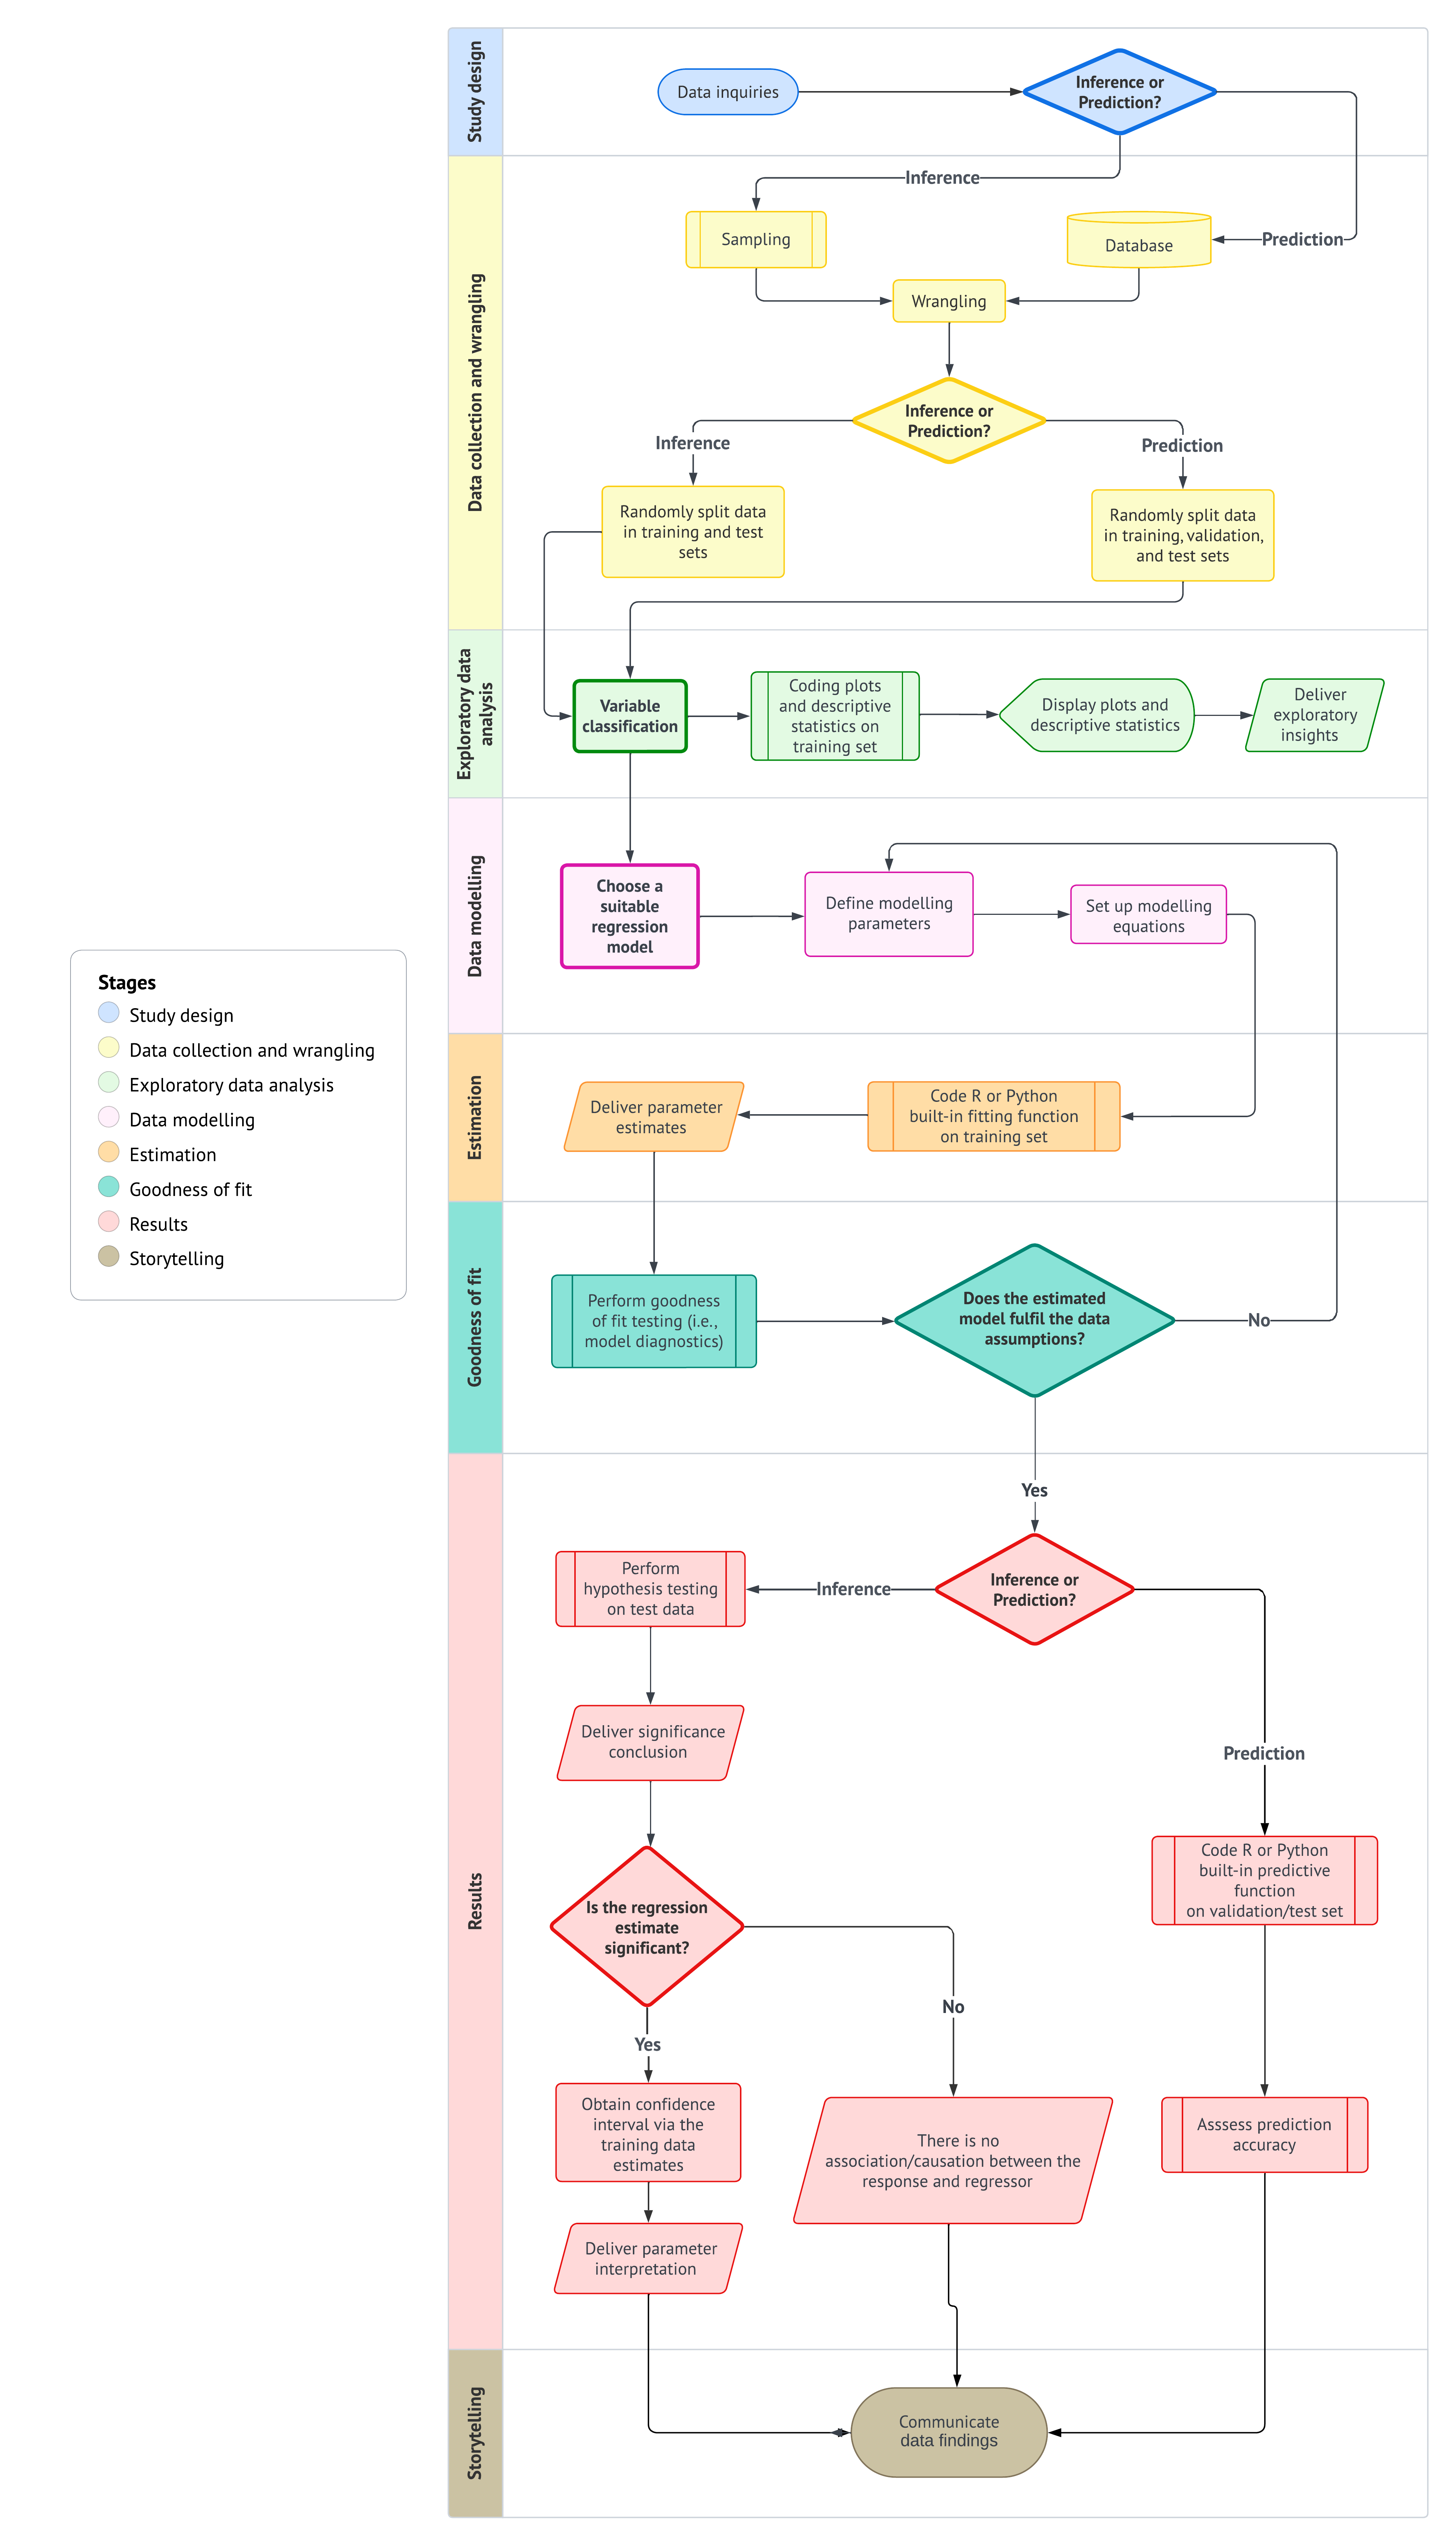
\includegraphics[width=10.41667in,height=\textheight]{book/img/data-science-workflow.png}

}

\caption{\label{fig-ds-workflow}Data science workflow for
\emph{inferential} and \emph{predictive} inquiries in regression
analysis and supervised learning, respectively.}

\end{figure}%

\subsection{Study Design}\label{sec-ds-workflow-study-design}

The first stage of this workflow is centered around defining the
\textbf{main statistical inquiries} we aim to address throughout the
data analysis process. As a data scientist, your primary task is to
translate these inquiries from the stakeholders into one of two
categories: \emph{inferential} or \emph{predictive}. This classification
determines the direction of your analysis and the methods you will use.

\begin{itemize}
\item
  \textbf{Inferential:} The objective here is to explore and quantify
  relationships of \emph{association} or \emph{causation} between
  explanatory variables (regressors) and the response variable within
  the context of the problem at hand. For example, you may seek to
  determine whether a specific marketing campaign (regressor)
  significantly impacts sales revenue (response) and, if so, by how
  much.
\item
  \textbf{Predictive:} In this case, the focus is on making accurate
  predictions about the response variable based on future observations
  of the regressors. Unlike inferential inquiries, where understanding
  the relationship between variables is key, the primary goal here is to
  maximize prediction accuracy. This approach is fundamental in machine
  learning. For instance, you might build a model to predict future
  sales revenue based on past marketing expenditures, without
  necessarily needing to understand the underlying relationship between
  the two.
\end{itemize}

\subsubsection{Example: Predicting Housing
Prices}\label{example-predicting-housing-prices}

To illustrate the study design stage, let's consider a simple example:
predicting housing prices in a specific city.

\begin{itemize}
\item
  If our goal is \emph{inferential}, we might be interested in
  understanding the relationship between various factors (like square
  footage, number of bedrooms, and proximity to schools) and housing
  prices. Specifically, we would ask questions like, ``How much does the
  number of bedrooms affect the price of a house, after accounting for
  other factors?''
\item
  If our goal is \emph{predictive}, we would focus on creating a model
  that can accurately predict the price of a house based on its
  features, regardless of whether we fully understand how each factor
  contributes to the price.
\end{itemize}

In both cases, the study design stage involves clearly defining these
objectives and determining the appropriate methods to address them. This
stage sets the foundation for all subsequent steps in the data science
workflow, as illustrated in Figure~\ref{fig-ds-workflow-study-design}.
Once the study design is established, the next stage is data collection
and wrangling.

\begin{figure}

\centering{

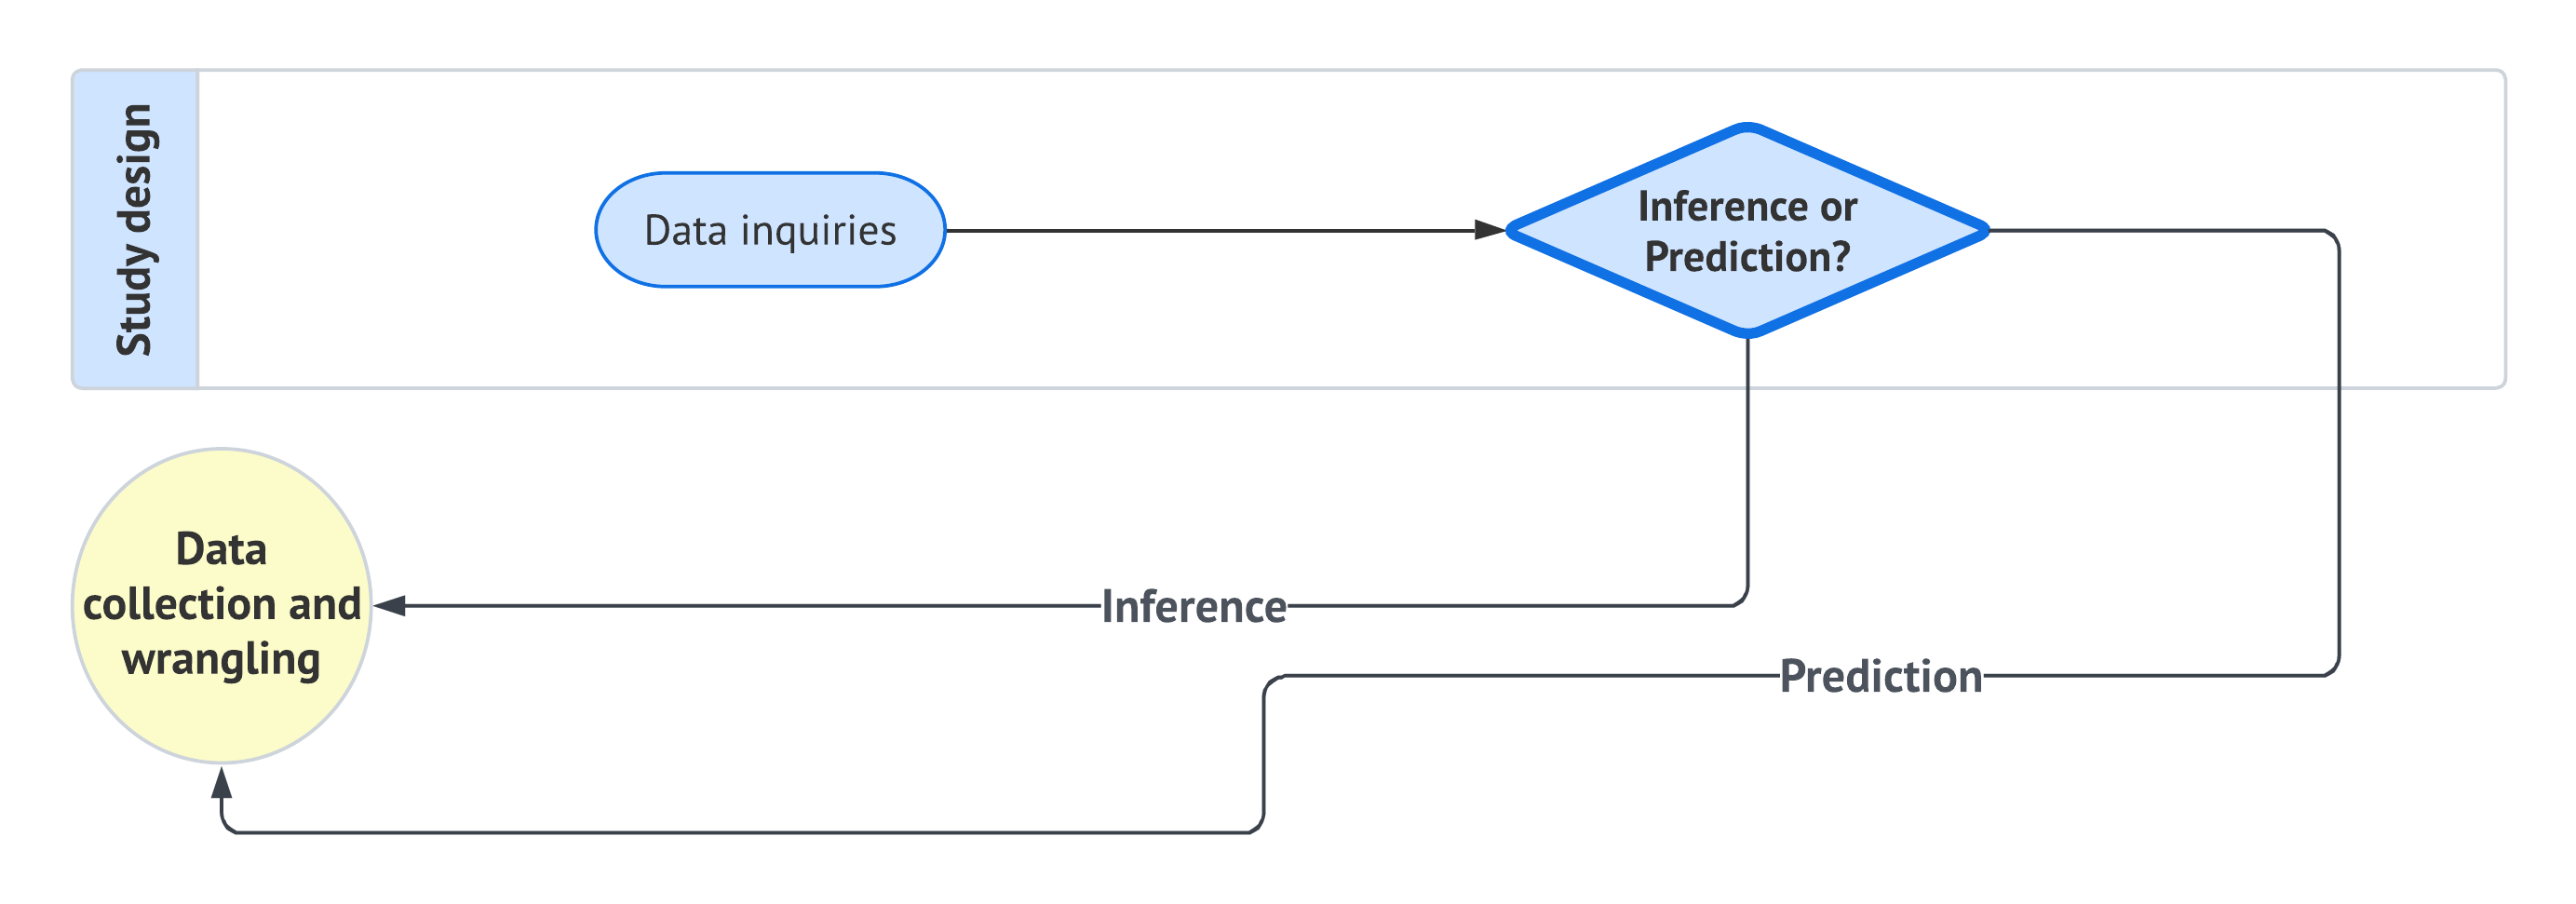
\includegraphics[width=6.97917in,height=\textheight]{book/img/study-design.png}

}

\caption{\label{fig-ds-workflow-study-design}\emph{Study design} stage
from the data science workflow in Figure~\ref{fig-ds-workflow}. This
stage is directly followed by \emph{data collection and wrangling}.}

\end{figure}%

\subsection{Data Collection and
Wrangling}\label{sec-ds-workflow-data-collection}

Once we have clearly defined our statistical questions, the next crucial
step is to collect the data that will form the basis of our analysis.
The way we collect this data is vital because it directly affects the
accuracy and reliability of our results:

\begin{itemize}
\tightlist
\item
  \textbf{For inferential inquiries}, we focus on understanding large
  groups or systems (populations) that we cannot fully observe. These
  populations are governed by characteristics (parameters) that we want
  to estimate. Because we can't study every individual in the
  population, we collect a smaller, representative subset called a
  sample. The method we use to collect this sample---known as
  \textbf{sampling}---is crucial. A proper sampling method ensures that
  our sample reflects the larger population, allowing us to make
  accurate generalizations (inferences) about the entire group. After
  collecting the sample, it's common practice to \textbf{randomly split
  the data into training and test sets}. This split allows us to build
  and validate our models, ensuring that the findings are robust and not
  overly tailored to the specific data at hand.
\end{itemize}

\begin{tcolorbox}[enhanced jigsaw, bottomrule=.15mm, breakable, colback=white, leftrule=.75mm, coltitle=black, rightrule=.15mm, bottomtitle=1mm, title=\textcolor{quarto-callout-tip-color}{\faLightbulb}\hspace{0.5em}{Tip \ref*{tip-sampling}: A Quick Debrief on Sampling!}, opacitybacktitle=0.6, toprule=.15mm, titlerule=0mm, arc=.35mm, colbacktitle=quarto-callout-tip-color!10!white, toptitle=1mm, colframe=quarto-callout-tip-color-frame, left=2mm, opacityback=0]

\quartocallouttip{tip-sampling} 

Although this book does not cover sampling methods in detail, it's
important to know that the way you collect your sample can greatly
influence your results. Depending on the problem, you might use
different techniques:

\begin{itemize}
\tightlist
\item
  \textbf{Simple Random Sampling:} Every individual in the population
  has an equal chance of being selected.
\item
  \textbf{Systematic Sampling:} You select individuals at regular
  intervals from a list of the population.
\item
  \textbf{Stratified Sampling:} You divide the population into subgroups
  (strata) and take a proportional sample from each subgroup.
\item
  \textbf{Clustered Sampling:} You divide the population into clusters
  and randomly select whole clusters for your sample.
\item
  Etc.
\end{itemize}

As in the case of Regression Analysis, statistical sampling is a vast
field, and we could spend a whole course on it. If you're interested in
learning more about these methods,
\href{https://webcat.library.ubc.ca/vwebv/holdingsInfo?bibId=2206157}{\emph{Sampling:
design and analysis}} by Lohr is a great resource.

\end{tcolorbox}

\begin{itemize}
\tightlist
\item
  \textbf{For predictive inquiries}, our goal is often to use existing
  data to make predictions about future events or outcomes. In these
  cases, we usually work with large datasets (databases) that have
  already been collected. Instead of focusing on whether the data
  represents a population (as in inferential inquiries), we focus on
  cleaning and preparing the data so that it can be used to train models
  that make accurate predictions. After wrangling the data, it is
  typically \textbf{split into training, validation, and test sets}. The
  training set is used to build the model, the validation set is used to
  tune model parameters, and the test set evaluates the model's final
  performance on unseen data.
\end{itemize}

\subsubsection{Example: Collecting Data for Housing Price
Predictions}\label{example-collecting-data-for-housing-price-predictions}

Let's continue with our housing price prediction example to illustrate
these concepts:

\begin{itemize}
\item
  \textbf{Inferential Approach:} Suppose we want to understand how the
  number of bedrooms affects housing prices in a city. To do this, we
  would collect a sample of house sales that accurately represents the
  city's entire housing market. For instance, we might use stratified
  sampling to ensure that we include houses from different neighborhoods
  in proportion to how common they are. After collecting the data, we
  would split it into training and test sets. The training set helps us
  build our model and estimate the relationship between variables, while
  the test set allows us to evaluate how well our findings generalize to
  new data.
\item
  Predictive Approach: If our goal is to predict the selling price of a
  house based on its features (like size, number of bedrooms, and
  location), we would gather a large dataset of recent house sales. This
  data might come from a real estate database that tracks the details of
  each sale. Before we can use this data to train a model, we would
  clean it by filling in any missing information, converting data to a
  consistent format, and making sure all variables are ready for
  analysis. After preprocessing, we would split the data into training,
  validation, and test sets. The training set would be used to fit the
  model, the validation set to fine-tune it, and the test set to assess
  how well the model can predict prices for houses it hasn't seen
  before.
\end{itemize}

As shown in Figure~\ref{fig-ds-workflow-data-collection-wrangling}, the
data collection and wrangling stage is fundamental to the workflow. It
directly follows the study design and sets the stage for exploratory
data analysis.

\begin{figure}

\centering{

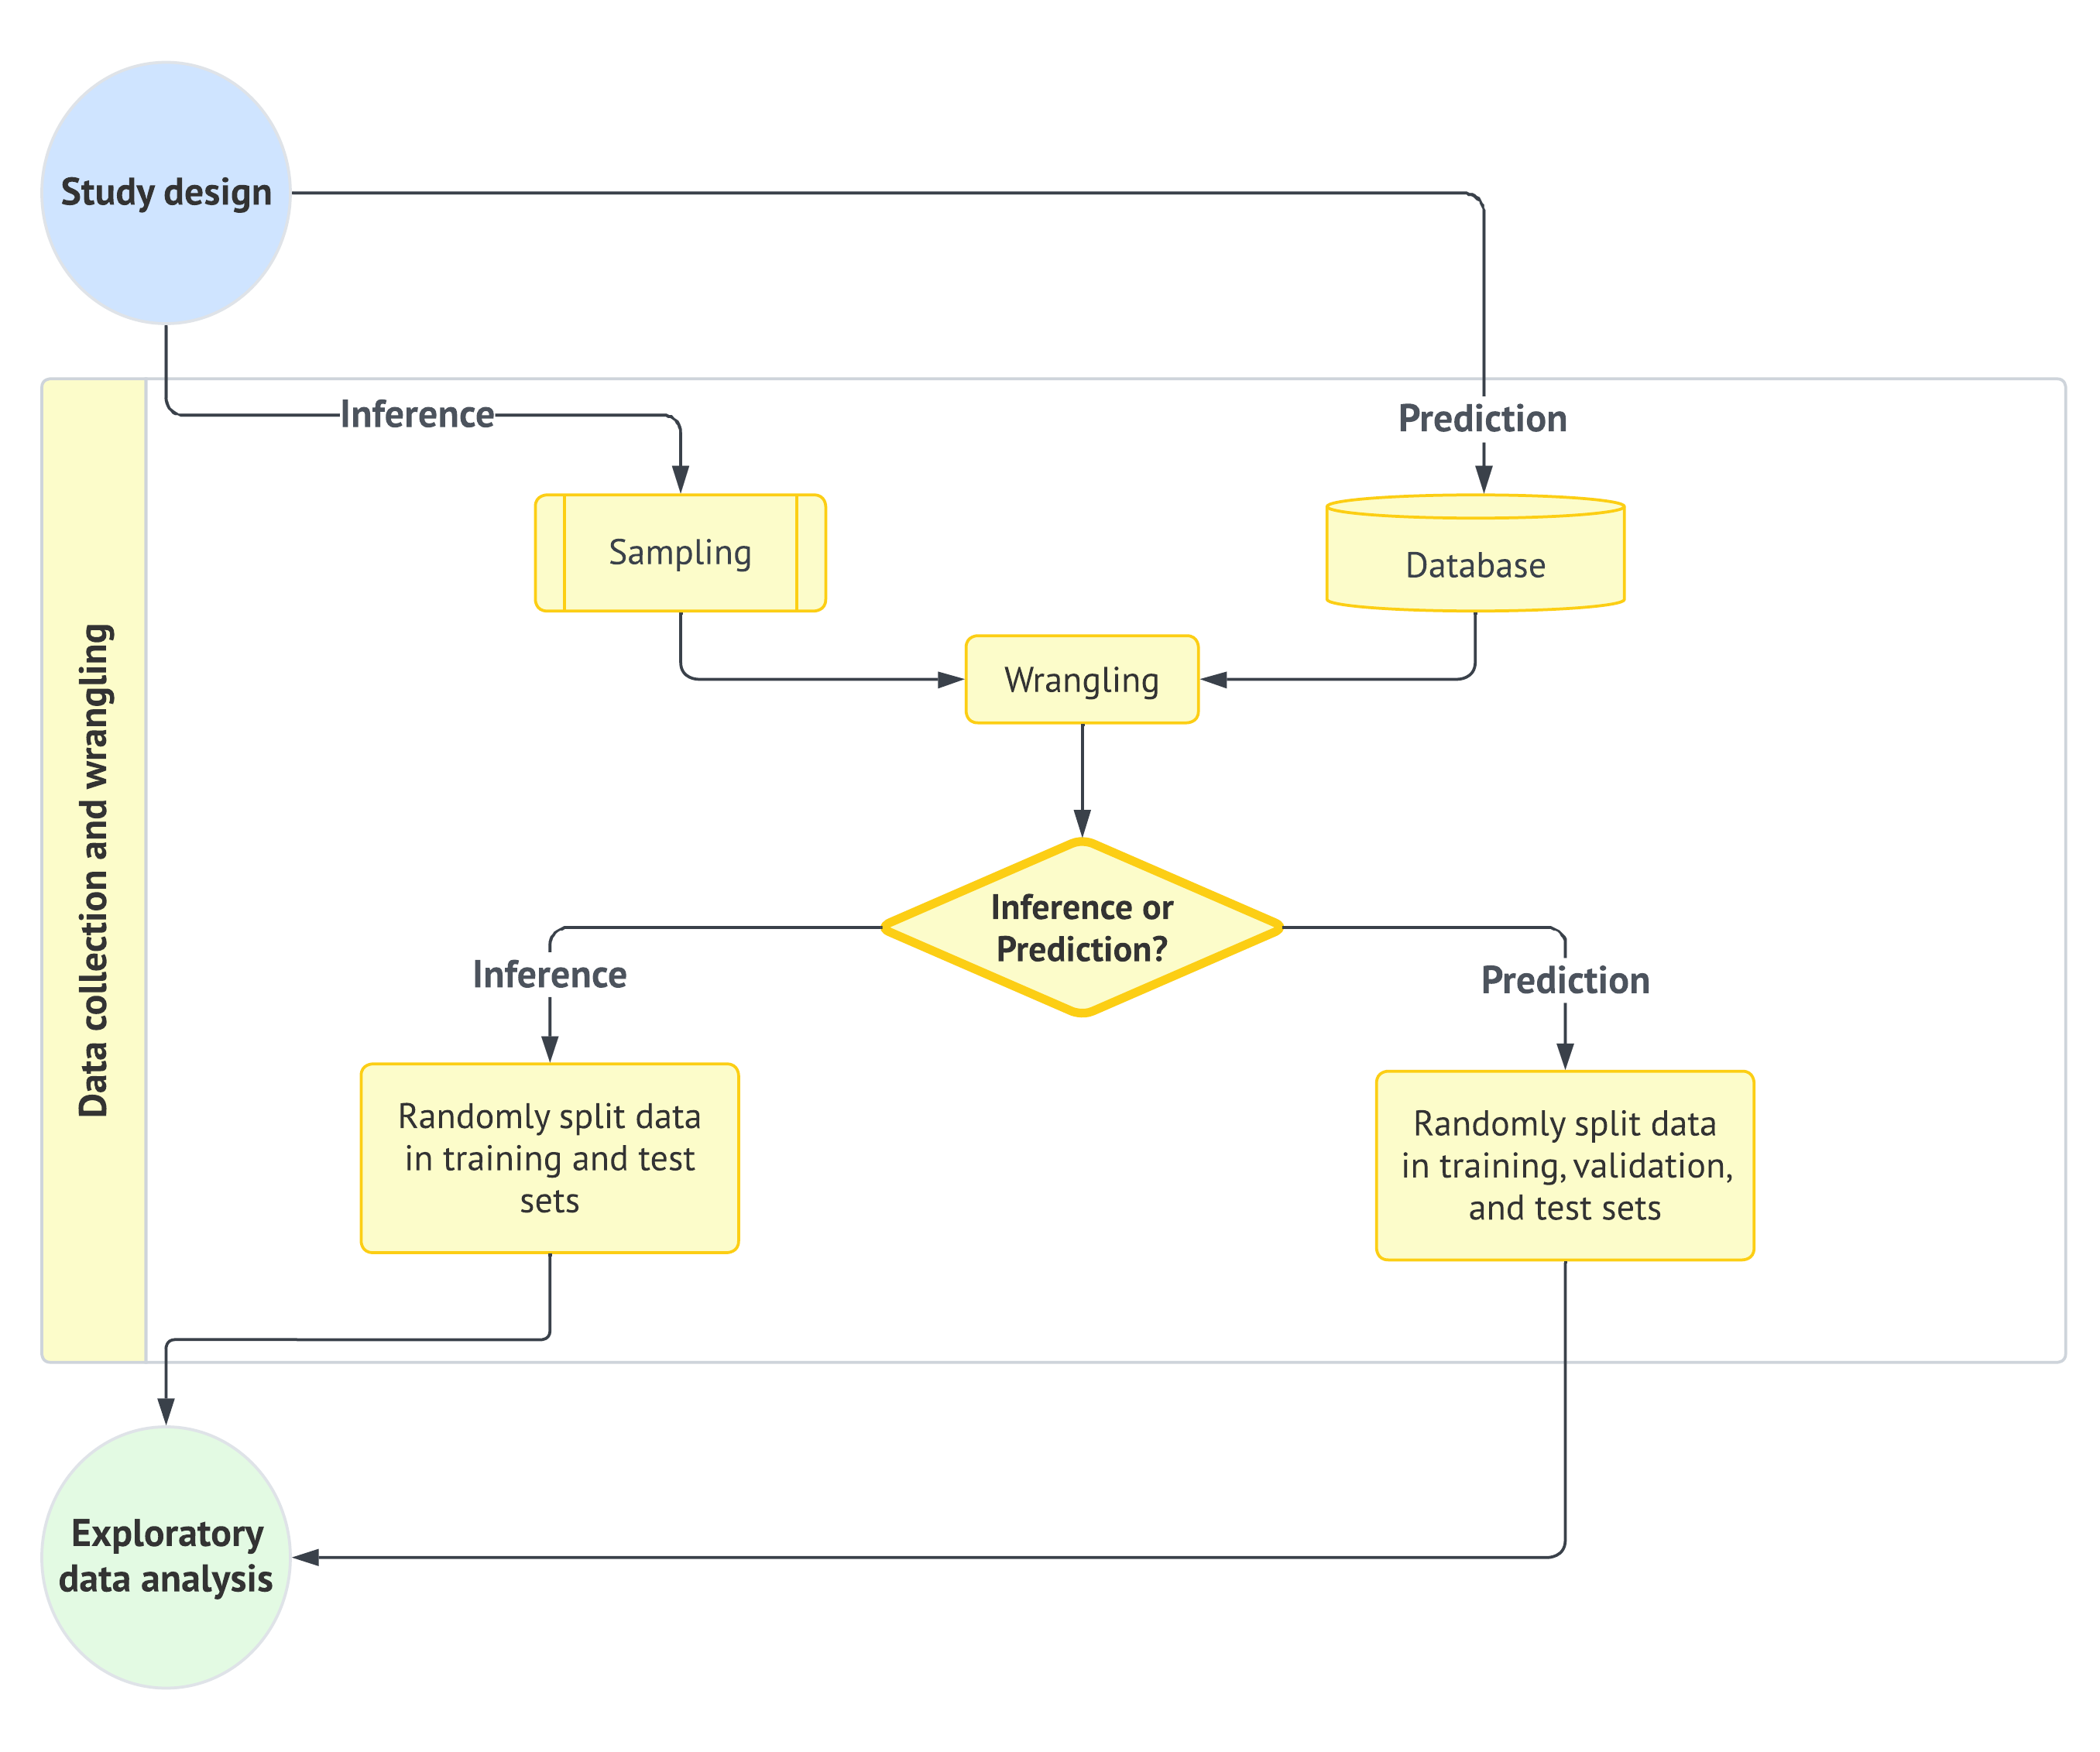
\includegraphics[width=6.97917in,height=\textheight]{book/img/data-collection-and-wrangling.png}

}

\caption{\label{fig-ds-workflow-data-collection-wrangling}\emph{Data
collection and wrangling} stage from the data science workflow in
Figure~\ref{fig-ds-workflow}. This stage is directly followed by
\emph{exploratory data analysis} and preceded by \emph{study design}.}

\end{figure}%

\subsection{Exploratory Data Analysis}\label{sec-ds-workflow-eda}

Before diving into data modeling, it's crucial to develop a deep
understanding of the relationships between the variables in your
training data. This is where the third stage of the data science
workflow---\textbf{Exploratory Data Analysis (EDA)}---comes into play.
EDA serves as a vital process that allows you to visualize and summarize
your data, uncover patterns, detect anomalies, and test key assumptions
that will inform your modeling decisions.

The first step in EDA is to classify your variables according to their
types. This classification is essential because it guides your choice of
analysis techniques and models. Specifically, you need to determine
whether each variable is discrete or continuous, and whether it has any
specific characteristics such as being bounded or unbounded.

\begin{itemize}
\tightlist
\item
  \textbf{Response Variable:}

  \begin{itemize}
  \tightlist
  \item
    Determine if your response variable is \emph{discrete} (e.g.,
    binary, count-based, categorical) or \emph{continuous}.
  \item
    If it is \emph{continuous}, consider whether it is \emph{bounded}
    (e.g., percentages that range between 0 and 100) or \emph{unbounded}
    (e.g., a variable like temperature that can take on a wide range of
    values).
  \end{itemize}
\item
  \textbf{Regressors}:

  \begin{itemize}
  \tightlist
  \item
    For each regressor, identify whether it is \emph{discrete} or
    \emph{continuous}.
  \item
    If a regressor is discrete, classify it further as binary,
    count-based, or categorical.
  \item
    If a regressor is continuous, determine whether it is bounded or
    unbounded.
  \end{itemize}
\end{itemize}

This classification step ensures that you are prepared to choose the
correct visualization and statistical methods for your analysis, as
different types of variables often require different approaches.

This classification step ensures that you are prepared to choose the
correct visualization and statistical methods for your analysis, as
different types of variables often require different approaches.

After classifying your variables, the next step is to create
visualizations and calculate descriptive statistics using your training
data. This involves coding plots that can reveal the underlying
distribution of each variable and the relationships between them. For
instance, you might create histograms to visualize distributions,
scatter plots to explore relationships between continuous variables, and
box plots to compare categorical variables against the response
variable.

Alongside these visualizations, it is important to calculate key
descriptive statistics such as the mean, median, and standard deviation.
These statistics provide a numerical summary of your data, offering
insights into central tendency and variability. You might also use a
correlation matrix to assess the strength of relationships between
continuous variables.

Once you have generated these plots and statistics, they should be
displayed in a clear and logical manner. The goal here is to interpret
the data and draw preliminary conclusions about the relationships
between variables. Presenting these findings effectively helps to
uncover key insights and prepares you for the modeling stage.

Finally, the insights gained from this exploratory analysis must be
clearly articulated. This involves summarizing the key findings and
considering their implications for the next stage of the workflow---data
modeling. Observing patterns, correlations, and potential outliers in
this stage will inform your modeling approach and ensure that it is
grounded in a thorough and informed analysis.

This structured approach to EDA is visually summarized in
Figure~\ref{fig-ds-workflow-eda}, illustrating the sequential steps from
variable classification to the delivery of exploratory insights.

\subsubsection{Example: EDA for Housing Price
Predictions}\label{example-eda-for-housing-price-predictions}

To illustrate the EDA process, let's apply it to the example of
predicting housing prices.

We start with \textbf{variable classification}:

\begin{itemize}
\tightlist
\item
  The \textbf{response variable} is the \emph{sale price of a house}, a
  continuous and unbounded variable.
\item
  The \textbf{regressors} include:

  \begin{itemize}
  \tightlist
  \item
    \emph{Number of bedrooms}: Discrete, count-based.
  \item
    \emph{Square footage}: Continuous and unbounded.
  \item
    \emph{Neighborhood type}: Discrete, categorical (e.g., urban,
    suburban, rural).
  \item
    \emph{Proximity to schools}: Continuous, potentially bounded by
    distance.
  \end{itemize}
\end{itemize}

Once the variables are classified, we move on to \textbf{coding plots
and calculating descriptive statistics}. Here are a couple of
visualizations that can be helpful in this context:

\begin{itemize}
\tightlist
\item
  A \textbf{histogram} of sale prices helps visualize the distribution
  and spot any outliers.
\item
  A \textbf{scatter plot} of square footage versus sale price shows the
  relationship, typically revealing a positive correlation.
\item
  \textbf{Box plots} compare sale prices across different neighborhood
  types, highlighting any variations in median prices.
\item
  \textbf{Descriptive statistics} like the mean and standard deviation
  provide a numerical summary, while a \textbf{correlation matrix} helps
  assess relationships between continuous variables like square footage
  and sale price.
\end{itemize}

Finally, in \textbf{displaying and interpreting results}, these plots
and statistics guide us in understanding the data:

\begin{itemize}
\tightlist
\item
  The histogram might show most houses fall within a mid-range price.
\item
  The scatter plot could confirm that larger houses generally sell for
  more.
\item
  Box plots may reveal that urban homes tend to have higher prices.
\end{itemize}

These \textbf{exploratory insights} help identify key predictors like
square footage and neighborhood type, and highlight any outliers that
may require further attention during modeling.

By following these steps, the EDA process in the housing price
prediction example lays a solid foundation for effective modeling,
ensuring that the key variables and their relationships are well
understood.

\begin{figure}

\centering{

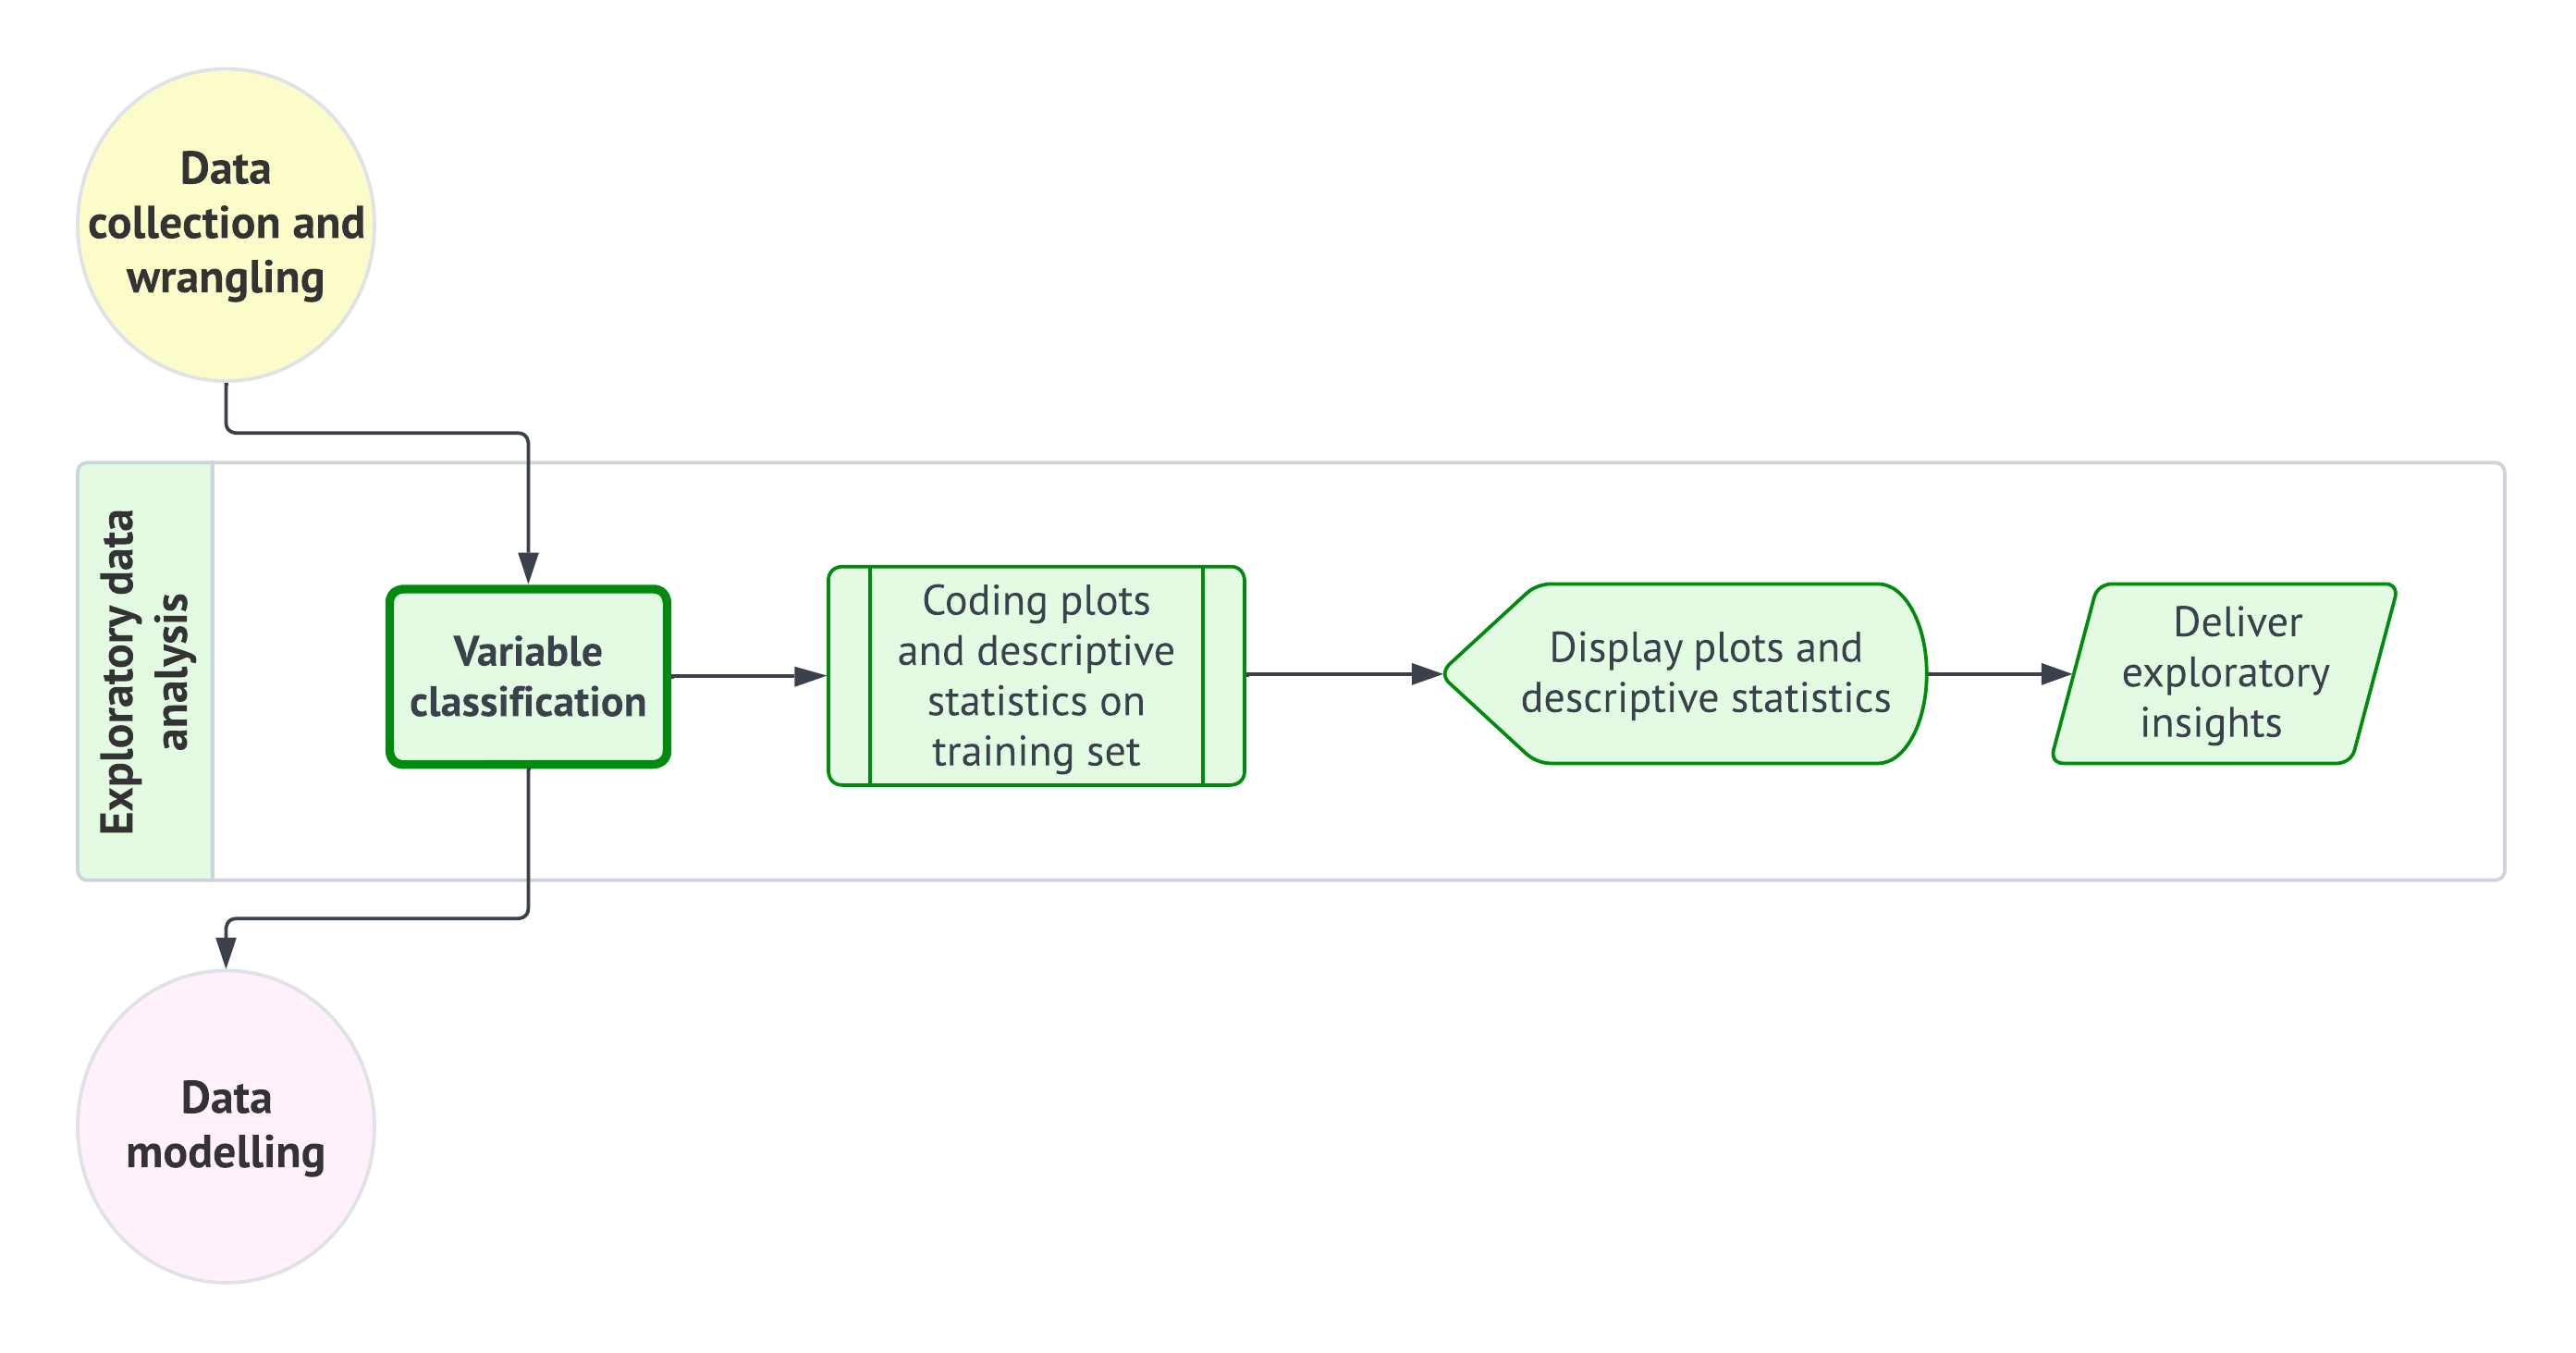
\includegraphics[width=6.97917in,height=\textheight]{book/img/eda.png}

}

\caption{\label{fig-ds-workflow-eda}\emph{Exploratory data analysis}
stage from the data science workflow in Figure~\ref{fig-ds-workflow}.
This stage is directly followed by \emph{data modelling} and preceded by
\emph{data collection and wrangling}.}

\end{figure}%

\subsection{Data Modelling}\label{sec-ds-workflow-modelling}

\begin{figure}

\centering{

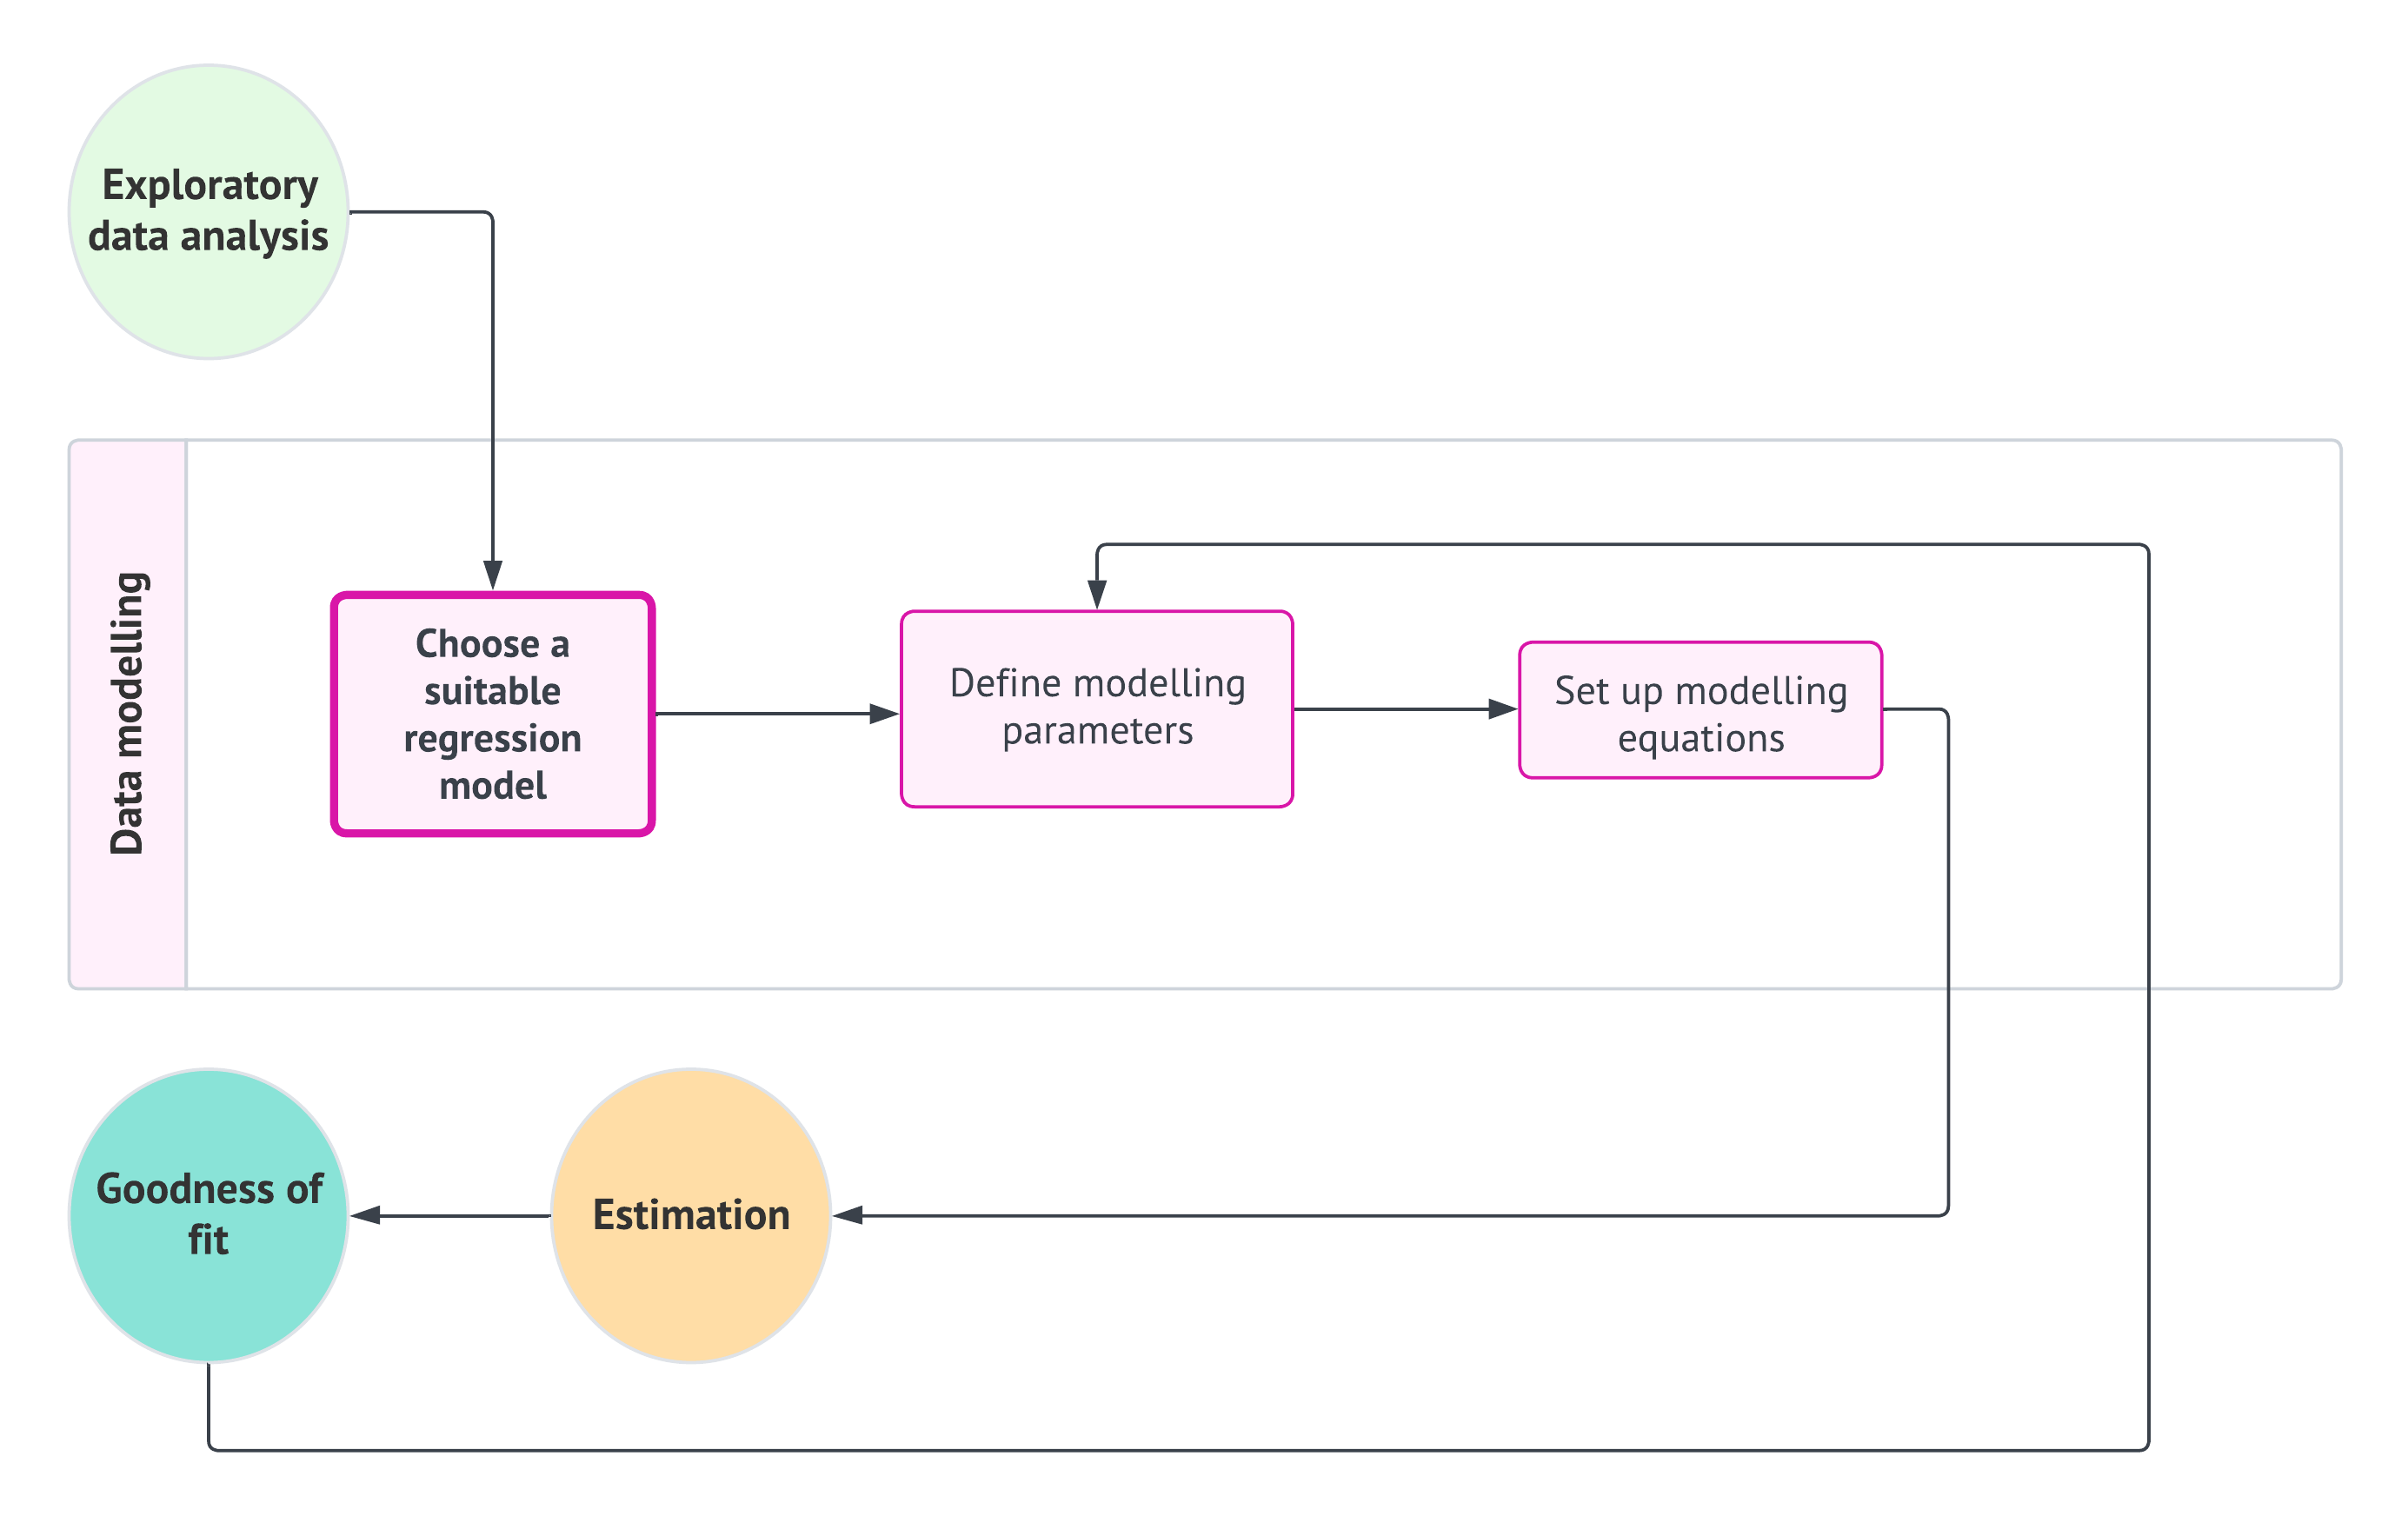
\includegraphics[width=6.97917in,height=\textheight]{book/img/data-modelling.png}

}

\caption{\label{fig-ds-workflow-data-modelling}\emph{Data modelling}
stage from the data science workflow in Figure~\ref{fig-ds-workflow}.
This stage is directly preceded by \emph{exploratory data analysis}. On
the other hand, it is directly followed by \emph{estimation} but
indirectly with \emph{goodness of fit}. If necessary, the \emph{goodness
of fit} stage could retake the process to \emph{data modelling}.}

\end{figure}%

\subsection{Estimation}\label{sec-ds-workflow-estimation}

\begin{figure}

\centering{

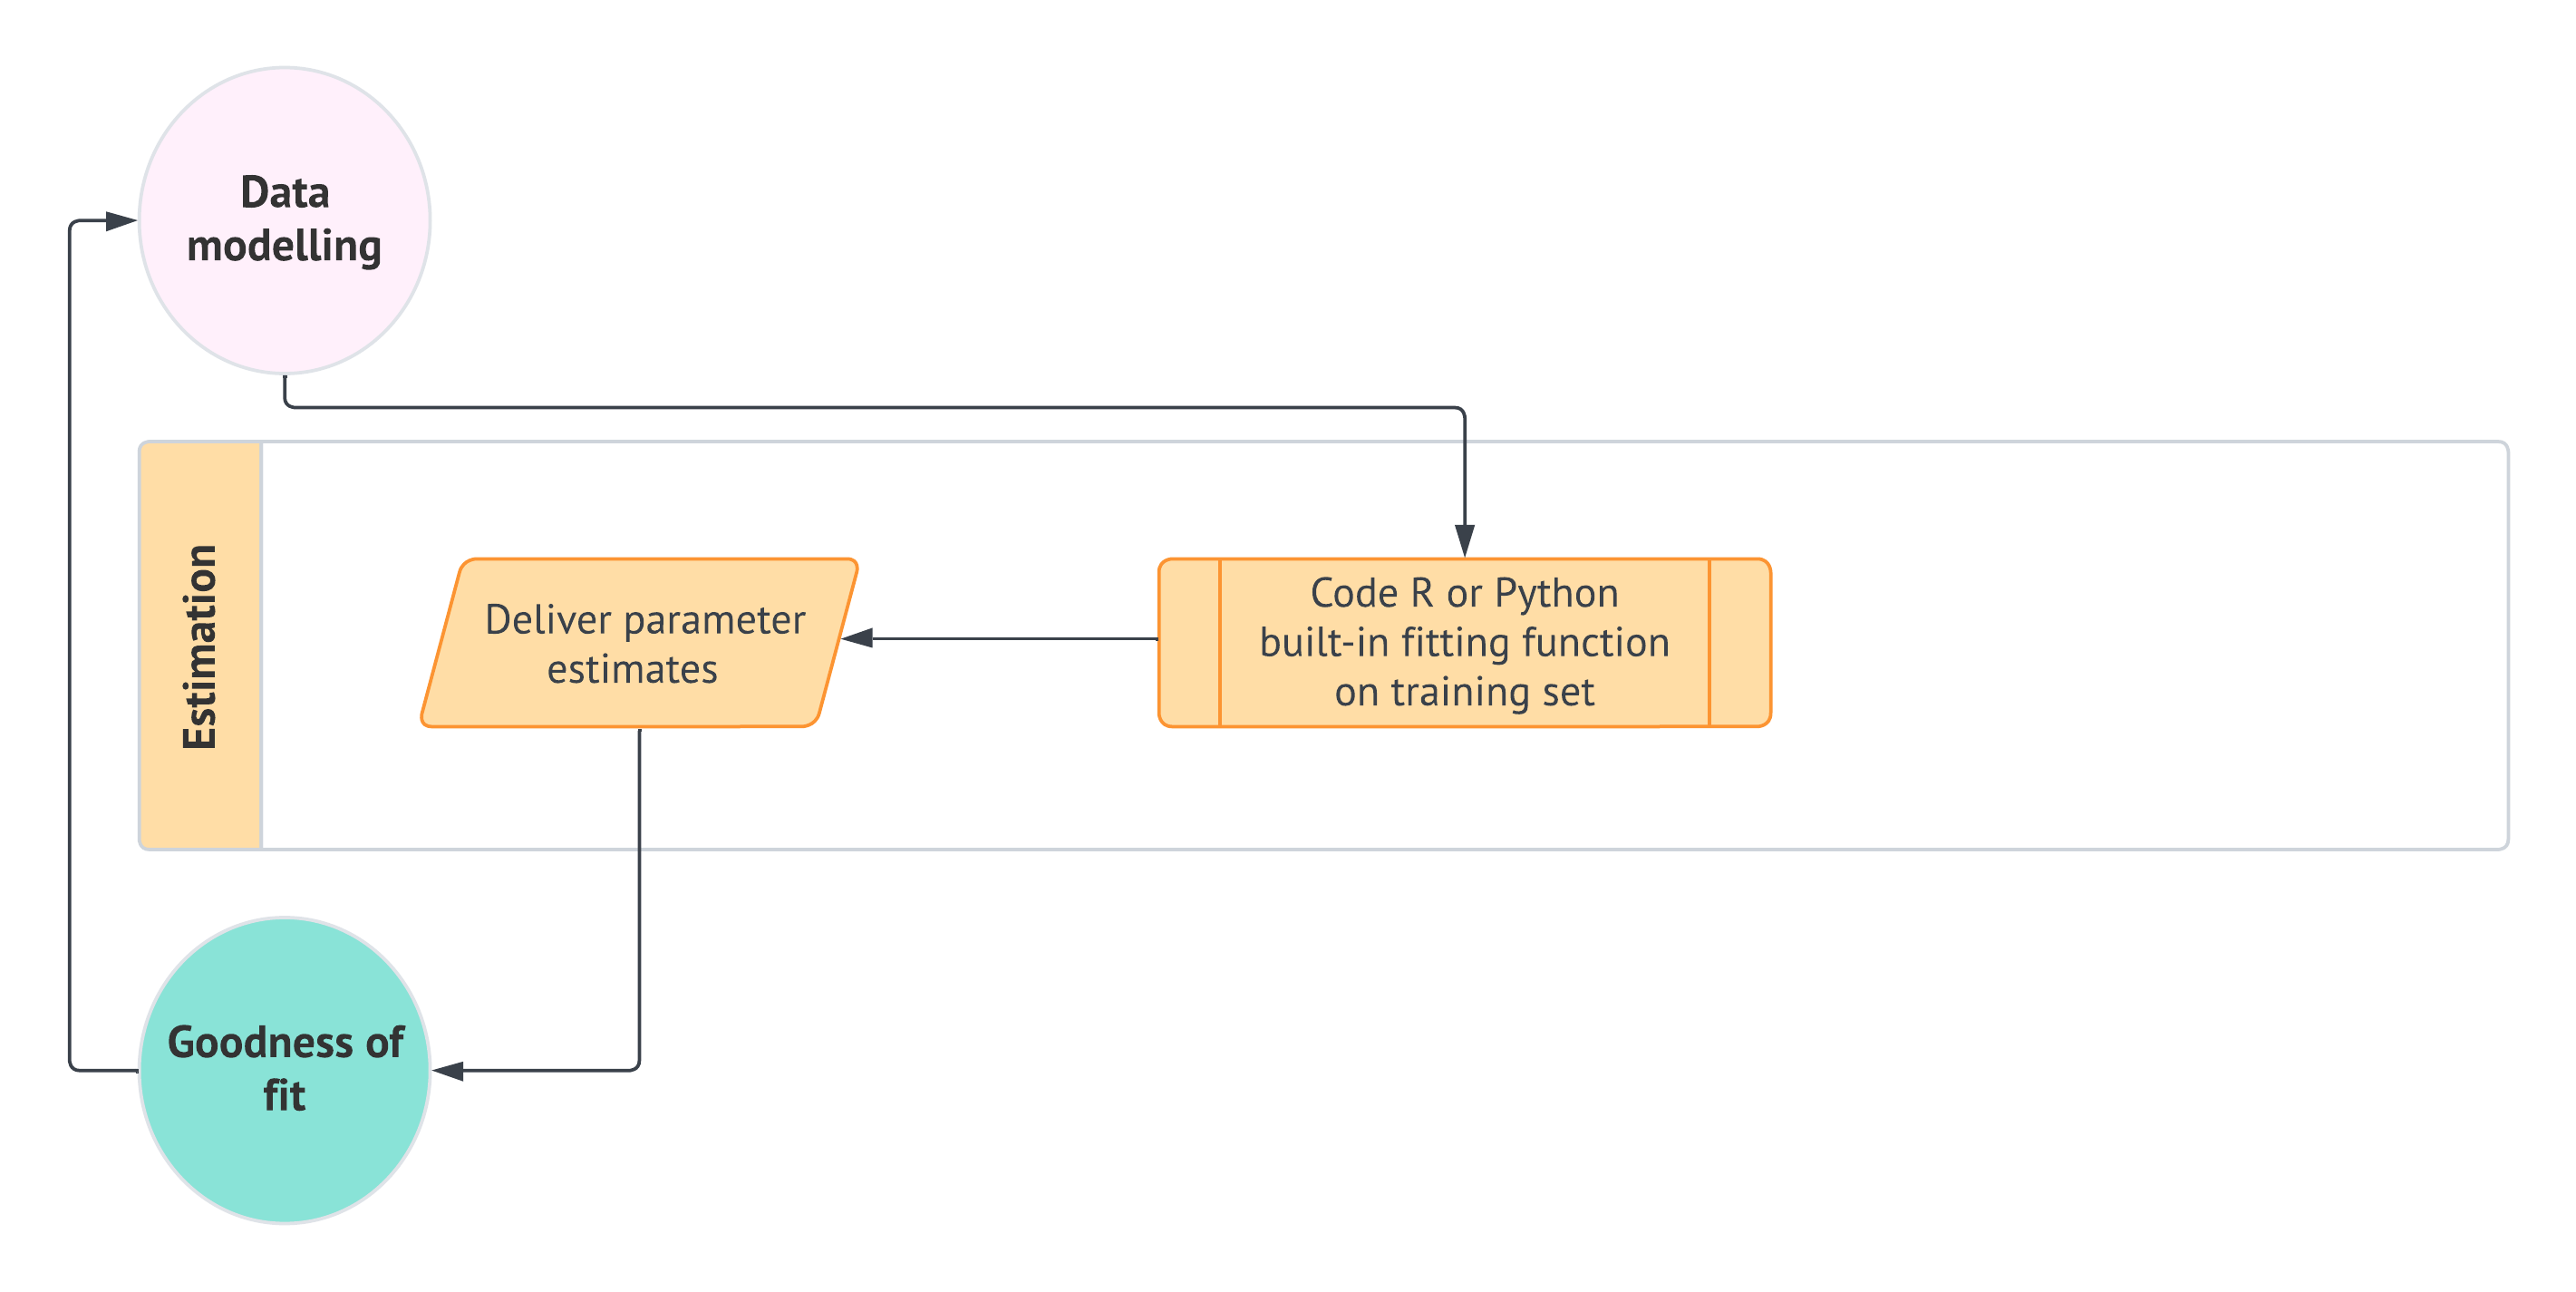
\includegraphics[width=6.97917in,height=\textheight]{book/img/estimation.png}

}

\caption{\label{fig-ds-workflow-estimation}\emph{Estimation} stage from
the data science workflow in Figure~\ref{fig-ds-workflow}. This stage is
directly preceded by \emph{data modelling} and followed by
\emph{goodness of fit}. If necessary, the \emph{goodness of fit} stage
could retake the process to \emph{data modelling} and then to
\emph{estimation}.}

\end{figure}%

\subsection{Goodness of Fit}\label{sec-ds-workflow-goodness-of-it}

\begin{figure}

\centering{

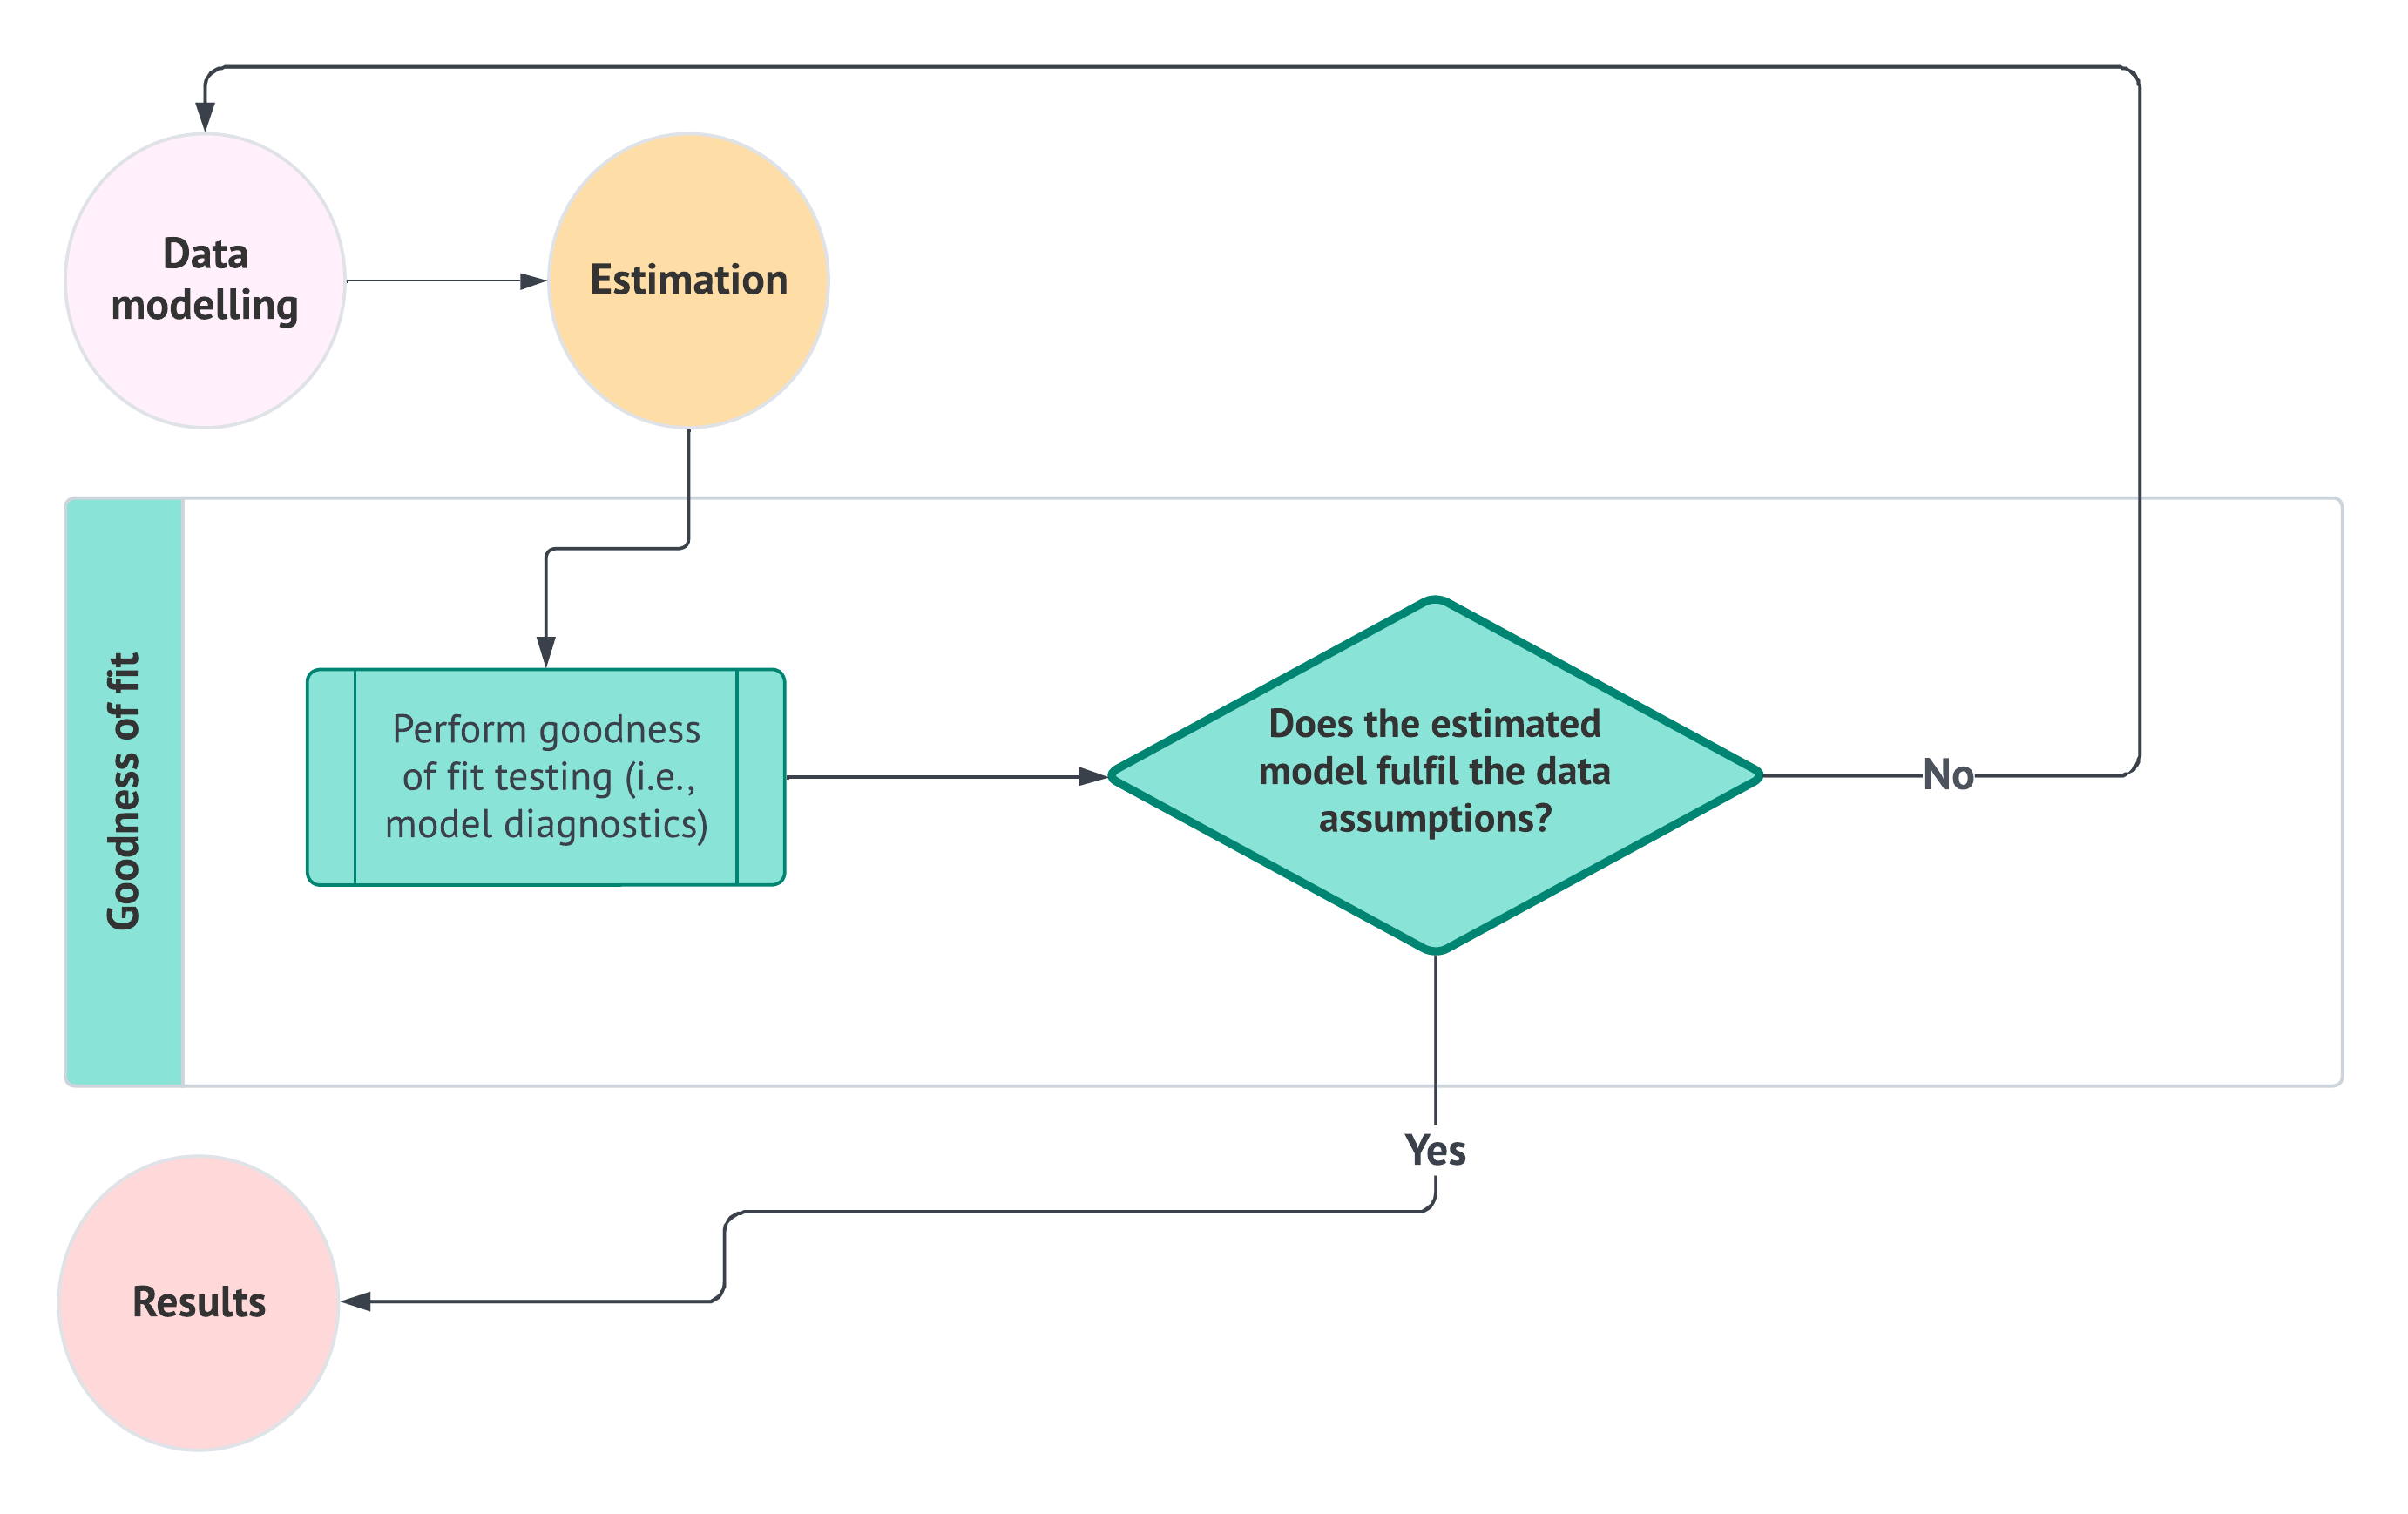
\includegraphics[width=6.97917in,height=\textheight]{book/img/goodness-of-fit.png}

}

\caption{\label{fig-ds-workflow-goodness-of-fit}\emph{Goodness of fit}
stage from the data science workflow in Figure~\ref{fig-ds-workflow}.
This stage is directly preceded by \emph{estimation} and followed by
\emph{results}. If necessary, the \emph{goodness of fit} stage could
retake the process to \emph{data modelling} and then to
\emph{estimation}.}

\end{figure}%

\subsection{Results}\label{sec-ds-workflow-results}

\begin{figure}

\centering{

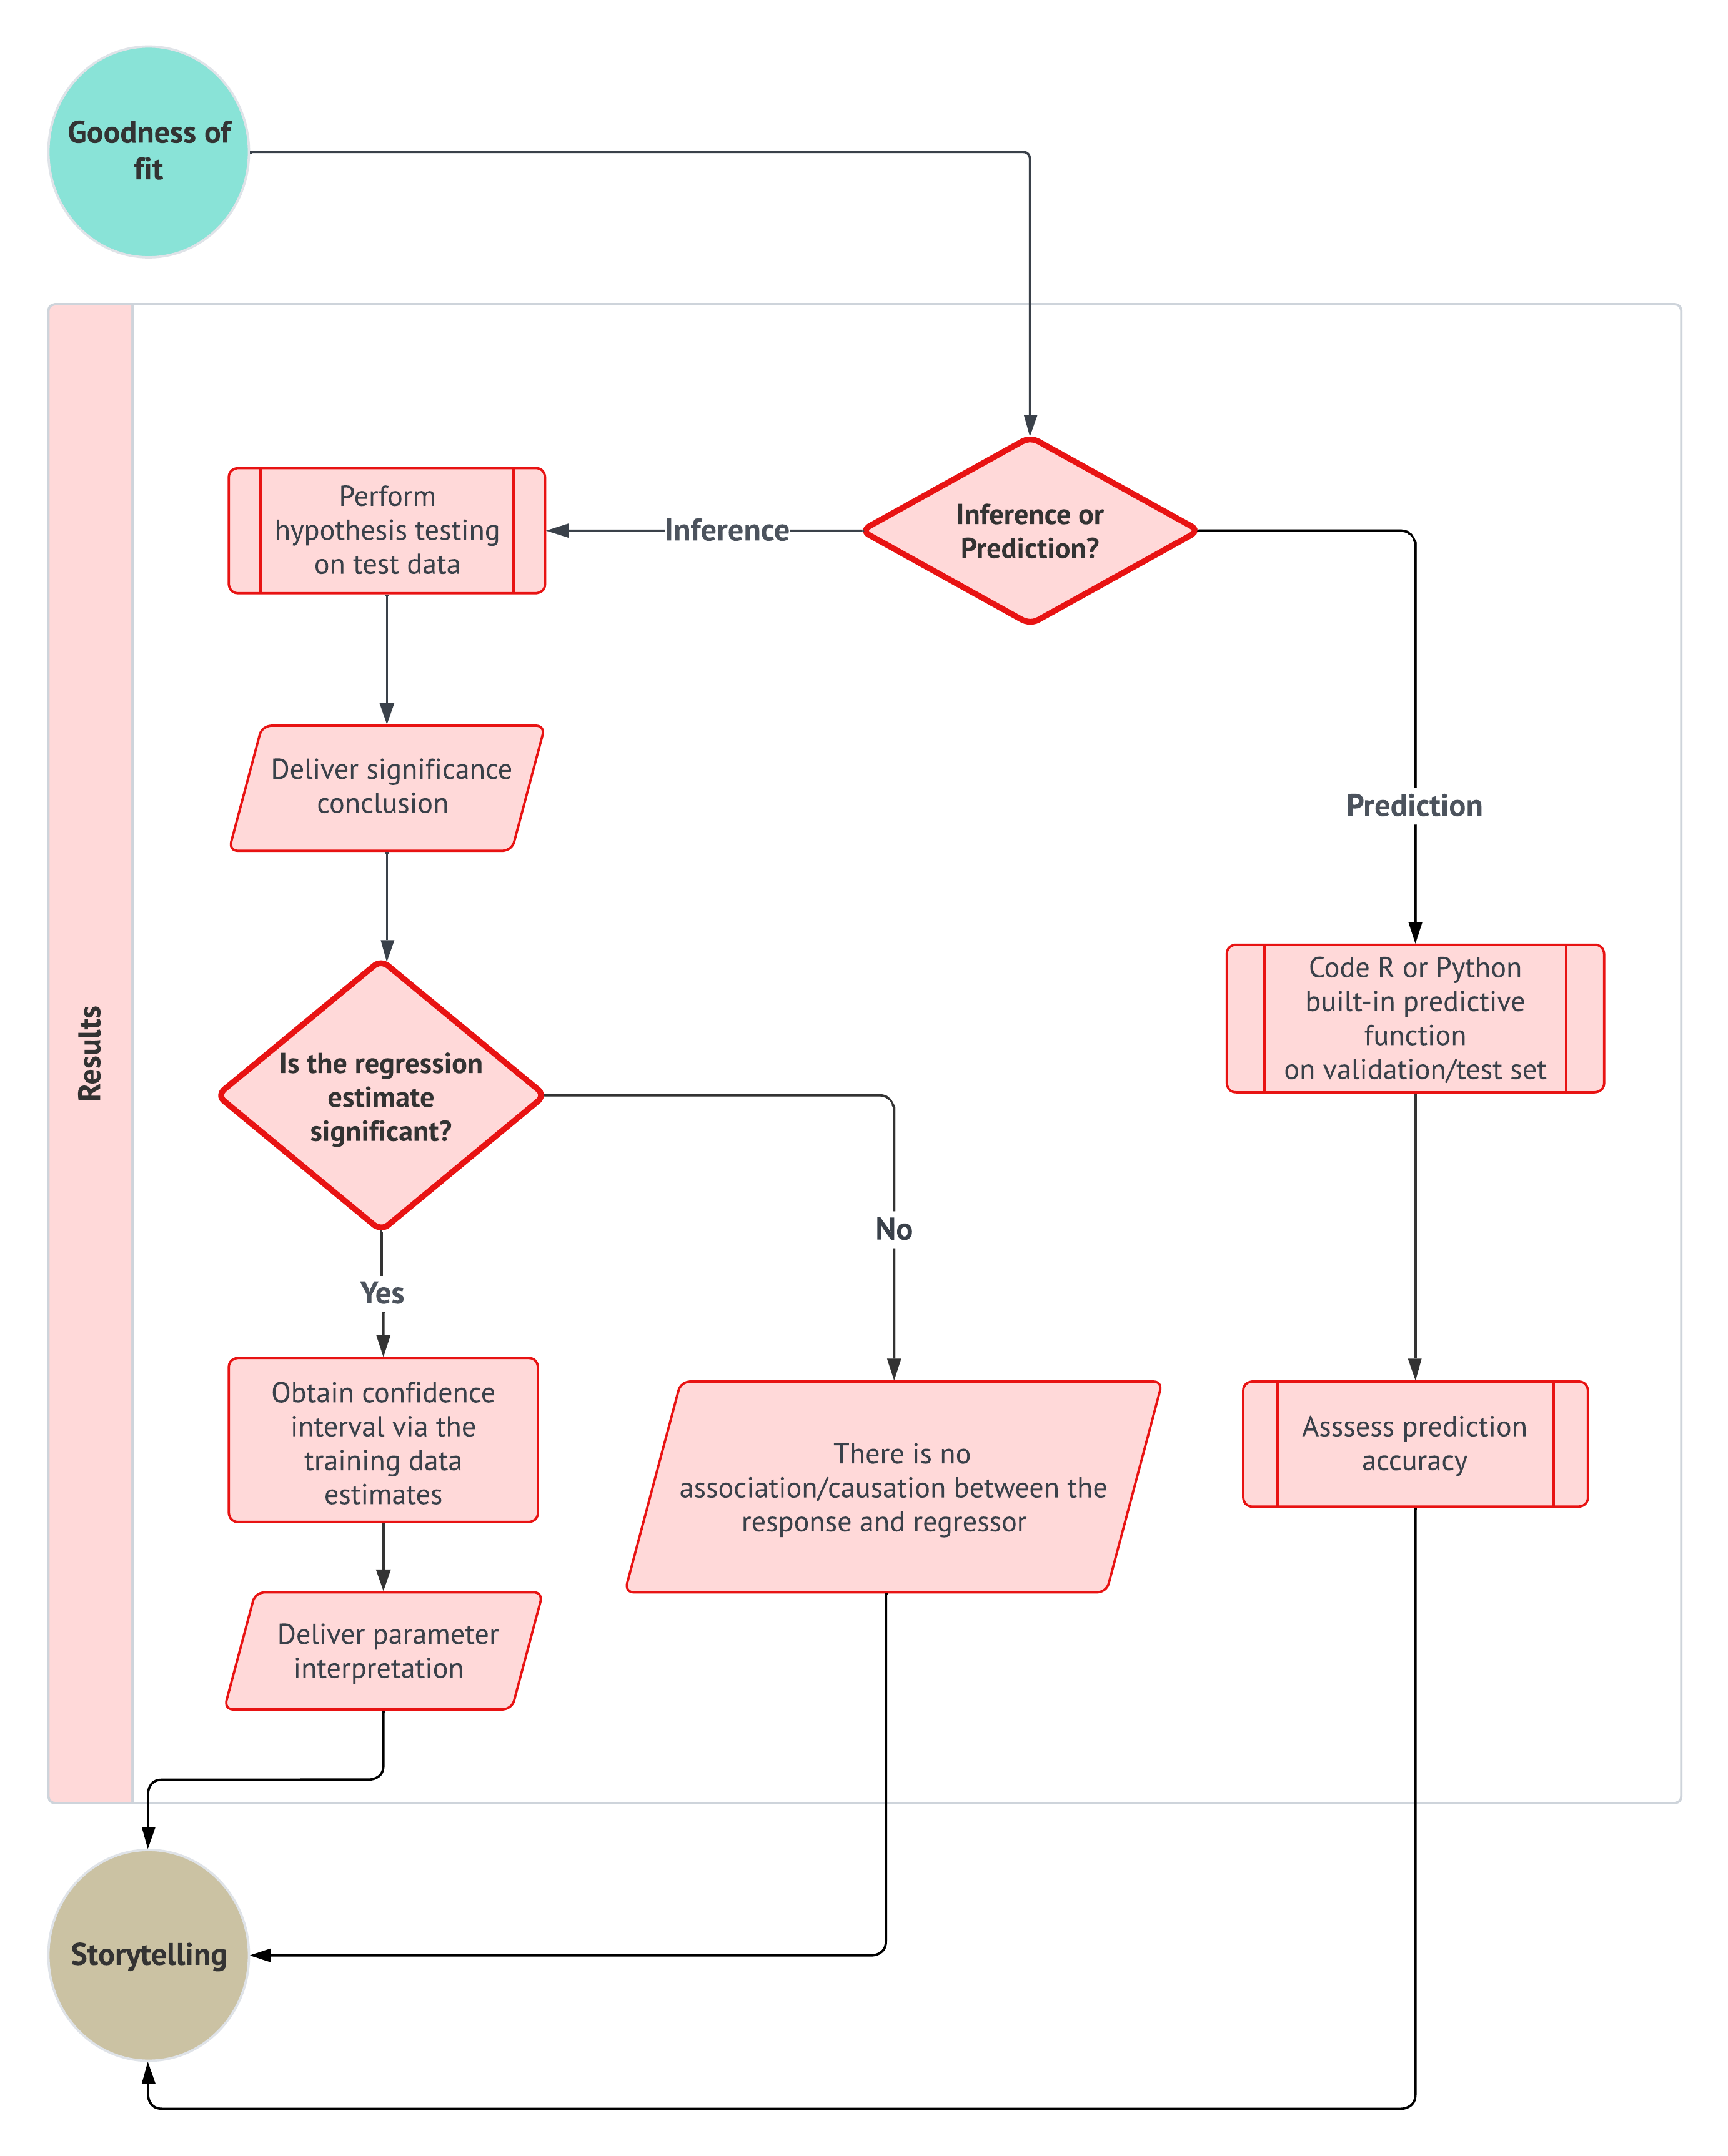
\includegraphics[width=6.97917in,height=\textheight]{book/img/results.png}

}

\caption{\label{fig-ds-workflow-results}\emph{Results} stage from the
data science workflow in Figure~\ref{fig-ds-workflow}. This stage is
directly followed by \emph{storytelling} and preceded by \emph{goodness
of fit}.}

\end{figure}%

\subsection{Storytelling}\label{sec-ds-workflow-storytelling}

\begin{figure}

\centering{

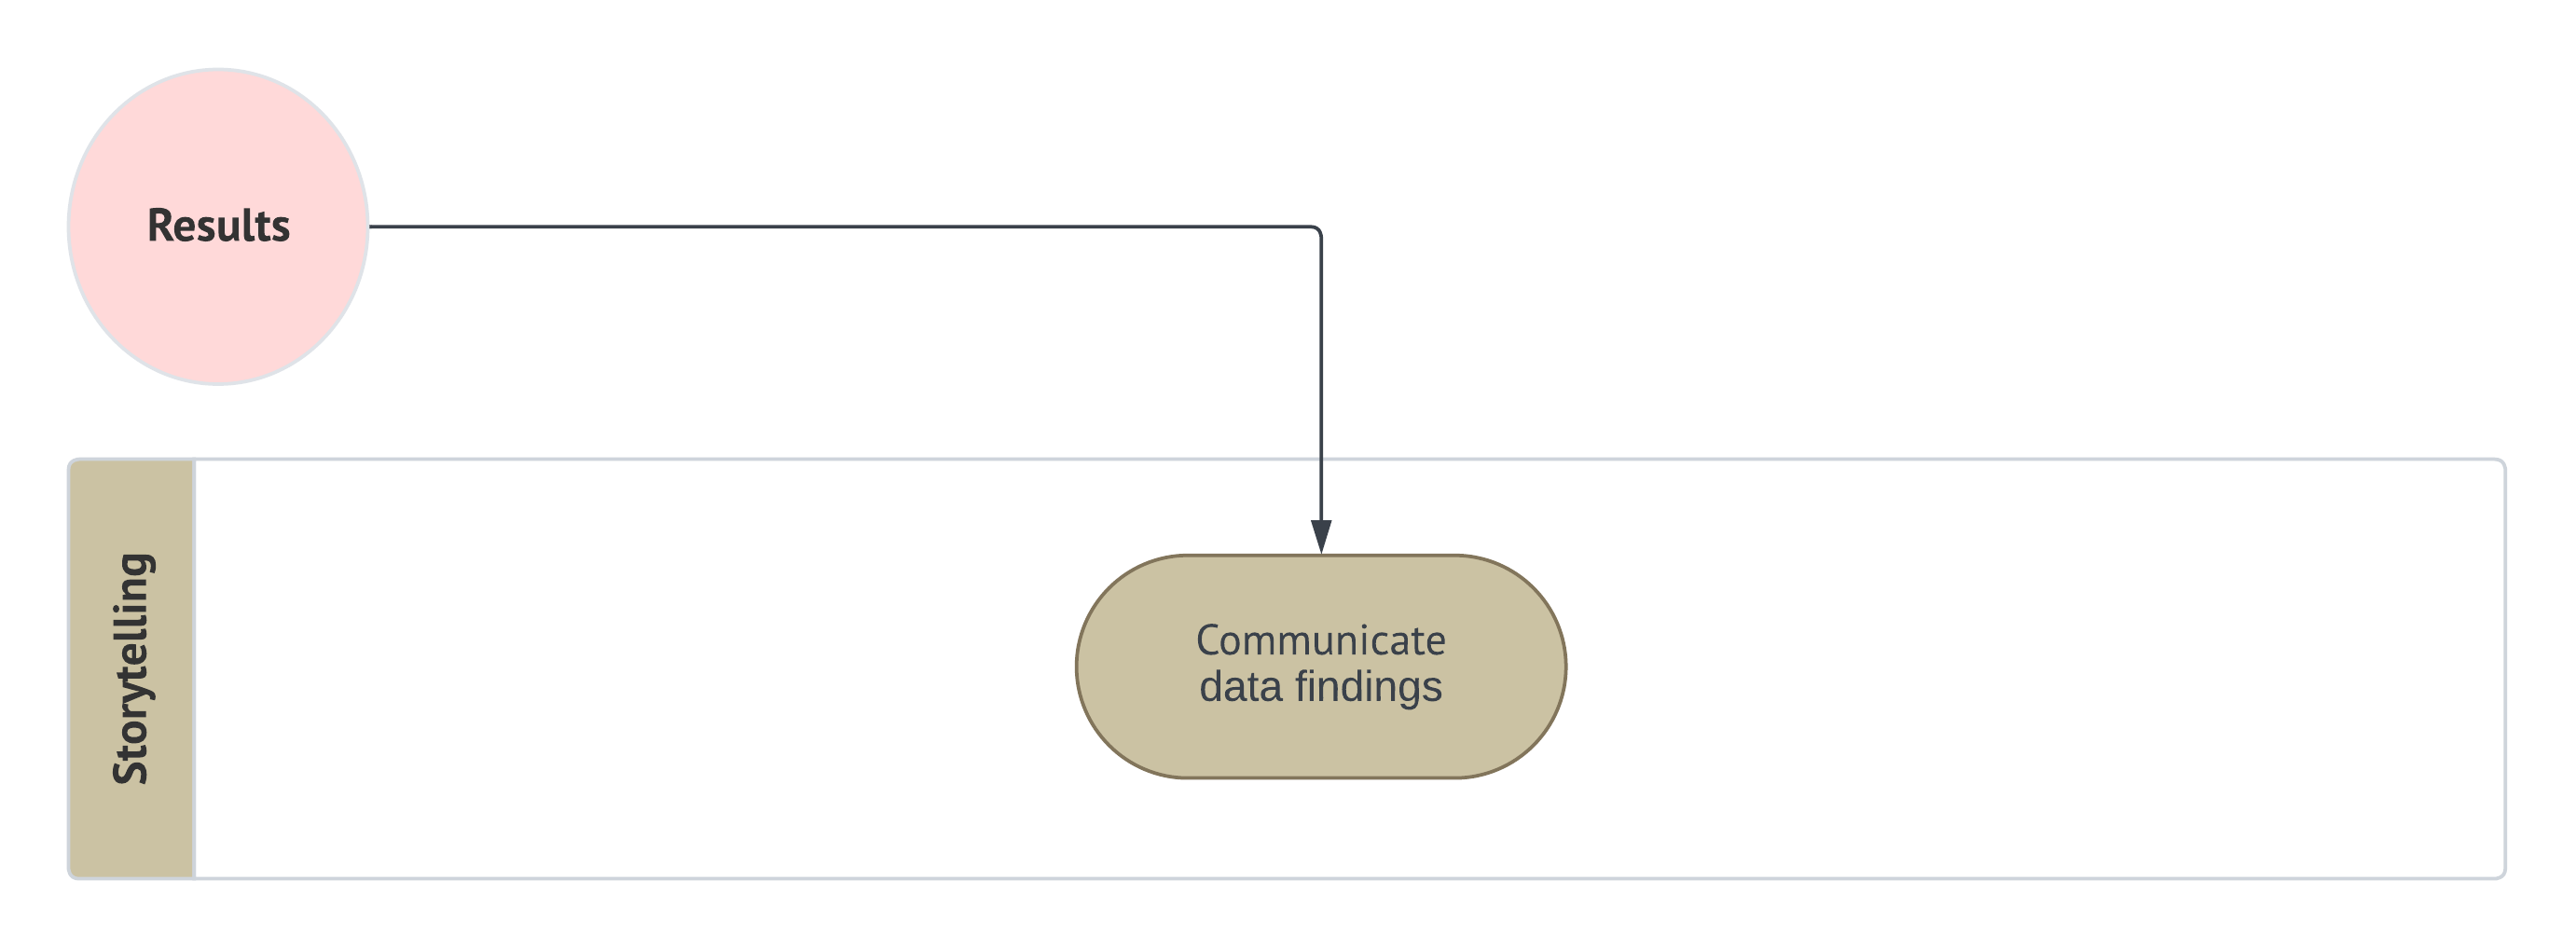
\includegraphics[width=6.97917in,height=\textheight]{book/img/storytelling.png}

}

\caption{\label{fig-ds-workflow-storytelling}\emph{Storytelling} stage
from the data science workflow in Figure~\ref{fig-ds-workflow}. This
stage preceded by \emph{results}.}

\end{figure}%

\section{Mindmap of Regression Analysis}\label{sec-regression-mindmap}

Having defined the necessary statistical aspects to execute a proper
supervised learning analysis, either \emph{inferential} or
\emph{predictive} across its seven sequential phases, we must dig into
the different approaches we might encounter in practice as regression
models. The nature of our outcome of interest will dictate any given
modelling approach to apply, depicted as clouds in
Figure~\ref{fig-regression-mindmap}. Note these regression models can be
split into two sets depending on whether the outcome of interest is
\emph{continuous} or \emph{discrete}. Therefore, under a probabilistic
view, identifying the nature of a given random variable is crucial in
regression analysis.

\begin{figure}

\centering{

\href{https://mermaid.live/edit\#pako:eNqVVd9v2jAQ_lciP4FEOgolDdE0aaVTN2kr1VhfKl6u8REsJT56dugPxP8-J6SCAgHqp-R8933fnc_nhYhJoohEprTMYDbWnsdEtvEXE0ZjFGmvsHnedw3pq1GmufodkLZK55Sbr4_85dswtzFluNqLIhWTbkzAeBPwOU-Rq6hi3etHyrVEuTZ9DMCXeAo6QR9SuxFXrOaQpdLAryXpbwRj_dFTDk5qaVmrbqwDb0lrTMCqOdZRpqQTH5jpuSD1WSXTHeobyDLYYtnwuWOaEVtnrCOZIceoLSS4DX2F9gDyKOe5mkPq_VNZbQYxpKglsG-dk9kiWCzugCFDyypeLj_ulQLW26WMd8b6mq5QR5ip2WHkAb1slKaC_AlvwNJ4O9DXysSMFo_1lJ1uZHhVdkRdYaSK0bfPtFOSkVNuVkzXYGGv-quNZqNEGVsV6EBNXLf5J0JTpqqCHAcfuDtj63LMDfLumf94ypVUxrWdQXlYzCAFRxhXau5IGUP6WKbDOfKJ-LfV_Su9PmR-Kr5HXPrfu8lxKusNamRI1VvleGJeD8jk_9KTFOwxhl3XoxwD55oQF8WuO043IrZP89ZVTG9G7JlhroP8PG3ukfknT-3n2q1Yq1l7nJP2clbRn-B7X42deTGU0jRrnIv7tj9AtESGnIGS7n1bFOFjYafoJoqI3KfECbi6jMVYL50r5JZGrzoWkeUcWyKfSXdS1woSN99ENIHUOOsMtIgW4kVEficMzy4vgiDo94Ner93vXrTEq7OfBxdnl0Ev7AVhOwyCdrBsiTcih3F-1u2e98NOEIT9sNvudDstgVJZ4j-rR7h8i0uShzKgULL8DwFMR-8}{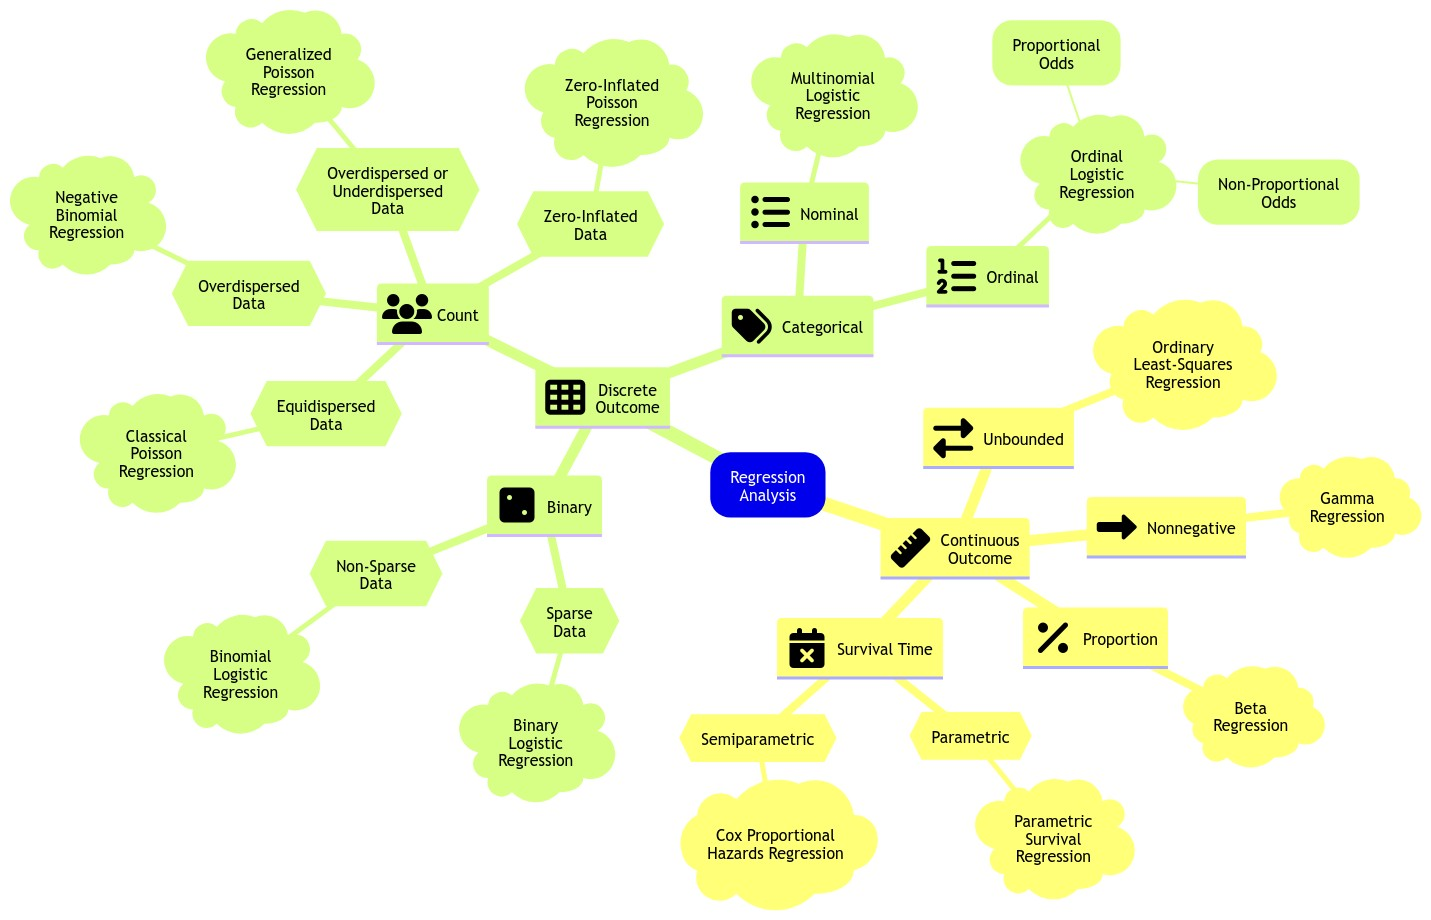
\includegraphics{index_files/mediabag/pako-eNqVVd9v2jAQ_lc.jpg}}

}

\caption{\label{fig-regression-mindmap}Regression analysis mindmap
depicting all modelling techniques to be explored in this book. These
techniques are split into two big sets: \emph{continuous} and
\emph{discrete} outcomes.}

\end{figure}%

That said, we will go beyond OLS regression and explore further
regression techniques. In practice, these techniques have been developed
in the statistical literature to address practical cases where the OLS
modelling framework and assumptions are not suitable anymore. Thus,
throughout this block, we will cover (at least) one new regression model
per lecture.

As we can see in the clouds of Figure~\ref{fig-regression-mindmap},
there are 13 regression models: 8 belonging to discrete outcomes and 5
to continuous outcomes. Each of these models is contained in a chapter
of this book, beginning with the most basic regression tool known as
ordinary least-squares in Chapter~\ref{sec-ols}. We must clarify that
the current statistical literature is not restricted to these 13
regression models. The field of regression analysis is vast, and one
might encounter more complex models to target certain specific
inquiries. Nonetheless, I consider these models the fundamental
regression approaches that any data scientist must be familiar with in
everyday practice.

Even though this book comprises 13 chapters, each depicting a different
regression model, we have split these chapters into two major subsets:
those with \emph{continuous} outcomes and those with \emph{discrete}
outcomes.

\bookmarksetup{startatroot}

\chapter{A Review on Probability and Frequentist Statistical
Inference}\label{sec-stats-review}

This chapter will delve into probability and frequentist statistical
inference. We can view these sections as a quick review of introductory
probability and statistics concepts. Moreover, this review will be
important to understanding the philosophy of modelling parameter
estimation as outlined in Section~\ref{sec-ds-workflow-estimation}.
Then, we will pave the way to the rationale behind statistical inference
in the \emph{results} stage (as in
Section~\ref{sec-ds-workflow-results}) in our workflow from
Figure~\ref{fig-ds-workflow}. Note that we aim to explain all these
statistical and probabilistic concepts in the most possible practical
way via a made-up case study throughout this chapter. Still, we will use
an appropriate level of jargon and will follow the colour convention
found in Appendix~\ref{sec-dictionary} along with \textbf{definition}
admonitions as in \textbf{?@imp-example}.

\begin{figure}[H]

{\centering 
\includegraphics[width=4.16667in,height=\textheight]{book/img/panda.png}

}

\caption{Image by
\href{https://pixabay.com/users/openclipart-vectors-30363/}{\emph{OpenClipart-Vectors}}
via
\href{https://pixabay.com/vectors/panda-cute-bear-blue-question-149818/}{\emph{Pixabay}}.}

\end{figure}%

Imagine you are an undergraduate engineering student. Moreover, last
term, you just took and passed your first course in probability and
statistics (inference included!) in an industrial engineering context.
Moreover, as it could happen while taking an introductory course in
probability and statistics, you used to feel quite overwhelmed by the
large amount of jargon and formulas one had to grasp and use regularly
for primary engineering fields such as quality control in a
manufacturing facility. \emph{Population parameters}, \emph{hypothesis
testing}, \emph{tests statistics}, \emph{significance level},
\emph{\(p\)-values}, and \emph{confidence intervals} (\textbf{do not
worry, our
\textcolor{blue}{statistical}/\textcolor{magenta}{machine learning}
scheme will come in later in this review}) were appearing here and
there! And to your frustration, you could never find a statistical
connection between all these inferential tools! Instead, you relied on
mechanistic procedures when solving assignments or exam problems.

For instance, when performing hypothesis testing for a two-sample
\(t\)-test, you struggled to reflect what the hypotheses were trying to
indicate for the corresponding population parameter(s) or how the test
statistic was related to these hypotheses. Moreover, your interpretation
of the resulting \(p\)-value and/or confidence interval was purely
mechanical with the inherent claim:

\begin{quote}
\emph{With a significance level \(\alpha = 0.05\), we reject (\textbf{or
fail to reject, if that is the case!}) the null hypothesis given
that\ldots{}}
\end{quote}

Truthfully, this whole mechanical way of doing statistics is not ideal
in a teaching, research or industry environment. Along~the same lines,
the above situation should also not happen when we learn key statistical
topics for the very first time as undergraduate students. That is why we
will investigate a more intuitive way of viewing probability and its
crucial role in statistical inference. This matter will help us deliver
more coherent storytelling (as in
Section~\ref{sec-ds-workflow-storytelling}) when presenting our results
in practice during any regression analysis to our peers or stakeholders.
Note that the role of probability also extends to model training (as in
Section~\ref{sec-ds-workflow-estimation}) when it comes to supervised
learning and not just regarding statistical inference.

Having said all this, it is time to introduce a statement that is key
when teaching hypothesis testing in an introductory statistical
inference course:

\begin{quote}
\textbf{In statistical inference, everything always boils down to
randomness and how we can control it!}
\end{quote}

That is quite a bold statement! Nonetheless, once one starts teaching
statistical topics to audiences not entirely familiar with the usual
field jargon, the idea of randomness always persists across many
different tools. And, of course, regression analysis is not an exception
at all since it also involves inference on population parameters of
interest! This is why we have allocated this section in the textbook to
explain core probabilistic and inferential concepts to pave the way to
its role in regression analysis.

\begin{tcolorbox}[enhanced jigsaw, bottomrule=.15mm, breakable, colback=white, leftrule=.75mm, coltitle=black, rightrule=.15mm, bottomtitle=1mm, title=\textcolor{quarto-callout-note-color}{\faInfo}\hspace{0.5em}{Note \ref*{nte-mechinical-clarification}: Heads-up on why we mean as a non-ideal mechanical analysis!}, opacitybacktitle=0.6, toprule=.15mm, titlerule=0mm, arc=.35mm, colbacktitle=quarto-callout-note-color!10!white, toptitle=1mm, colframe=quarto-callout-note-color-frame, left=2mm, opacityback=0]

\quartocalloutnte{nte-mechinical-clarification} 

The reader might need clarification on why the mechanical way of
performing hypothesis testing is considered \textbf{non-ideal}, mainly
when the term \textbf{cookbook} is used in the book's title. The
\textbf{cookbook} concept here actually refers to a homogenized recipe
for data modelling, as seen in the workflow from
Figure~\ref{fig-ds-workflow}. However, there's a crucial distinction
between this and the non-ideal mechanical way of hypothesis testing.

On the one hand, the non-ideal mechanical way refers to \textbf{the use
of a tool without understanding the rationale of what this tool stands
for}, resulting in vacuous and standard statements that we would not be
able to explain any way further, such as the statement we previously
indicated:\\

\begin{quote}
\emph{With a significance level \(\alpha = 0.05\), we reject (\textbf{or
fail to reject, if that is the case!}) the null hypothesis given
that\ldots{}}\\
\end{quote}

What if a stakeholder of our analysis asks us in plain words what a
significance level means? Why are we phrasing our conclusion on the null
hypothesis and not directly on the alternative one? As a data scientist,
one should be able to explain why the whole inference process yields
that statement without misleading the stakeholders' understanding.
\textbf{For sure, this also implicates appropriate communication skills
that cater to general audiences rather than just statistical ones.}\\

Conversely, the data modelling workflow in Figure~\ref{fig-ds-workflow}
involves stages that necessitate a comprehensive and precise
understanding of our analysis. Progressing to the next stage without a
complete grasp of the current one risks perpetuating false insights,
potentially leading to faulty data storytelling of the entire analysis.

\end{tcolorbox}

Finally, even though this book has suggested reviews related to the
basics of probability via different distributions and the fundamentals
of frequentist statistical inference as stated in \textbf{Audience and
Scope}, we will retake essential concepts as follows:

\begin{itemize}
\tightlist
\item
  The role of \emph{random variables} and \emph{probability
  distributions} and the governance of \emph{population (or system)
  parameters} (i.e., the so-called Greek letters we usually see in
  statistical inference and regression analysis).
  Section~\ref{sec-basics-prob} will explore these topics more in detail
  while connecting them to the subsequent inferential terrain under a
  \emph{frequentist context}.
\item
  When delving into supervised learning and regression analysis, we
  might wonder how randomness is incorporated into \emph{model fitting}
  (i.e., \emph{parameter estimation}). That is quite a fascinating
  aspect, implemented via a crucial statistical tool known as
  \emph{maximum likelihood estimation}. This tool is heavily related to
  the concept of \emph{loss function} in supervised learning.
  Section~\ref{sec-mle} will explore these matters in more detail and
  how the idea of a \emph{random sample} is connected to this estimation
  tool.
\item
  Section~\ref{sec-basics-inf} will explore the basics of
  \emph{hypothesis testing} and its intrinsic components such as
  \emph{null} and \emph{alternative hypotheses}, \emph{type I} and
  \emph{type II} errors, \emph{test statistic}, \emph{standard error},
  \emph{\(p\)-value}, and \emph{confidence interval}.
\item
  Finally, Section~\ref{sec-sup-learning-regression} will briefly
  discuss the connections between supervised learning and regression
  analysis regarding terminology.
\end{itemize}

Without further ado, let us start with reviewing core concepts in
probability via quite a tasty example.

\section{Basics of Probability}\label{sec-basics-prob}

In terms of regression analysis and its supervised learning counterpart
(either on an \textbf{inferential} or \textbf{predictive} framework),
\textcolor{blue}{probability} can be viewed as the solid foundation on
which more complex tools, including estimation and
\textcolor{blue}{hypothesis testing}, are built upon. Under this
foundation, our data is coming from a given \textcolor{blue}{population}
or system of interest. Moreover, the \textcolor{blue}{population} or
system is assumed to be governed by \textcolor{blue}{parameters} which,
as data scientists or researchers, they are of their best interest to
study. That said, the terms \textcolor{blue}{population} and
\textcolor{blue}{parameter} will pave the way to our first statistical
definitions.

\begin{tcolorbox}[enhanced jigsaw, bottomrule=.15mm, breakable, colback=white, leftrule=.75mm, coltitle=black, rightrule=.15mm, bottomtitle=1mm, title=\textcolor{quarto-callout-important-color}{\faExclamation}\hspace{0.5em}{Important \ref*{imp-population}: Definition of population}, opacitybacktitle=0.6, toprule=.15mm, titlerule=0mm, arc=.35mm, colbacktitle=quarto-callout-important-color!10!white, toptitle=1mm, colframe=quarto-callout-important-color-frame, left=2mm, opacityback=0]

\quartocalloutimp{imp-population} 

It is a \textbf{whole collection of individuals or items} that share
\textbf{distinctive attributes}. As data scientists or researchers, we
are interested in studying these attributes, which we assume are
\textbf{governed} by \textcolor{blue}{parameters}. In practice, we must
be \textbf{as precise as possible} when defining our given
\textcolor{blue}{population} such that we would frame our entire data
modelling process since its very early stages. Examples of a
\textcolor{blue}{population} could be the following:

\begin{itemize}
\tightlist
\item
  \emph{Children between the ages of 5 and 10 years old in states of the
  American West Coast.}
\item
  \emph{Customers of musical vinyl records in the Canadian provinces of
  British Columbia and Alberta.}
\item
  \emph{Avocado trees grown in the Mexican state of Michoacán.}
\item
  \emph{Adult giant pandas in the Southwestern Chinese province of
  Sichuan.}
\item
  \emph{Mature açaí palm trees from the Brazilian Amazonian jungle.}
\end{itemize}

\begin{figure}[H]

{\centering 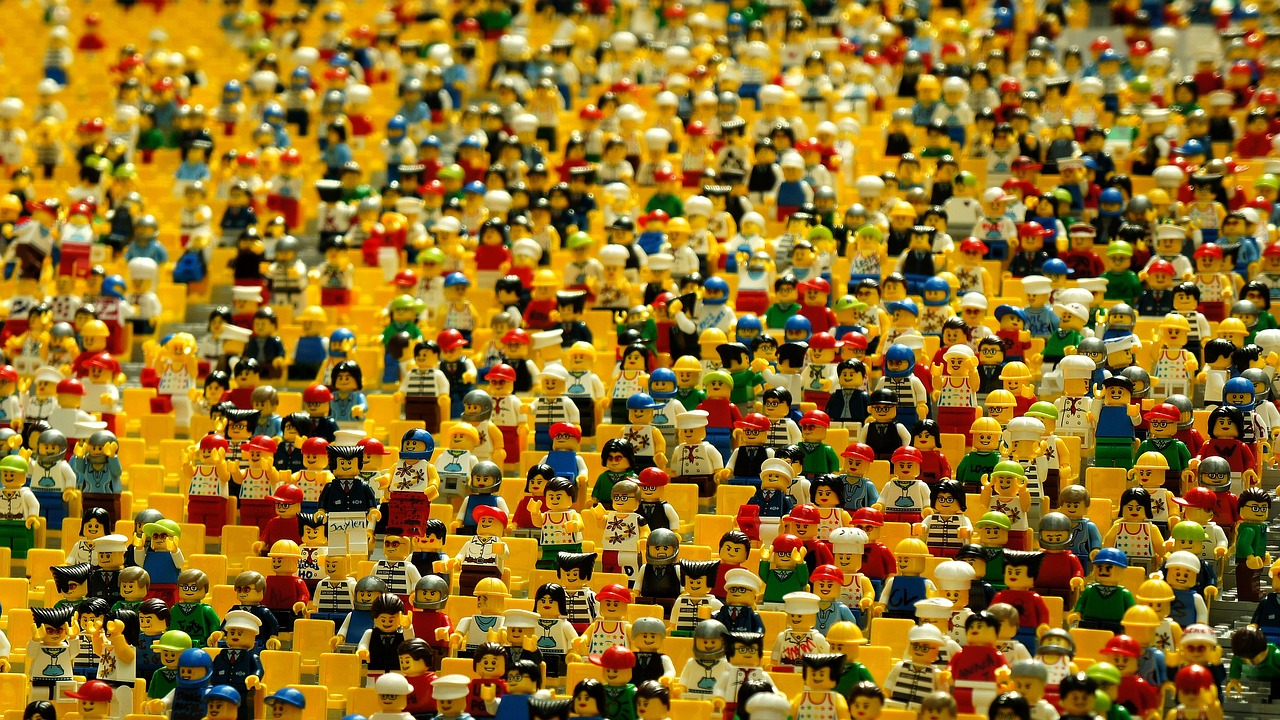
\includegraphics[width=5.72917in,height=\textheight]{book/img/lego.jpg}

}

\caption{Image by
\href{https://pixabay.com/users/eak_kkk-907811/?utm_source=link-attribution&utm_medium=referral&utm_campaign=image&utm_content=1044891}{\emph{Eak
K.}} via
\href{https://pixabay.com/photos/lego-toys-figurines-crowd-many-1044891/}{\emph{Pixabay}}.}

\end{figure}%

Note that the term \textcolor{blue}{population} could be exchanged for
the term \textbf{system}, given that certain contexts do not
particularly refer to individuals or items. Instead, these contexts
could refer to \textbf{processes} whose attributes are also governed by
\textcolor{blue}{parameters}. Examples of a \textbf{system} could be the
following:

\begin{itemize}
\tightlist
\item
  \emph{The production of cellular phones from a given model in a set of
  manufacturing facilities.}
\item
  \emph{The sale process in the Vancouver franchises of a well-known ice
  cream parlour.}
\item
  \emph{The transit cycle during rush hours on weekdays in the twelve
  lines of Mexico City's subway.}
\end{itemize}

\end{tcolorbox}

\begin{tcolorbox}[enhanced jigsaw, bottomrule=.15mm, breakable, colback=white, leftrule=.75mm, coltitle=black, rightrule=.15mm, bottomtitle=1mm, title=\textcolor{quarto-callout-important-color}{\faExclamation}\hspace{0.5em}{Important \ref*{imp-parameter}: Definition of parameter}, opacitybacktitle=0.6, toprule=.15mm, titlerule=0mm, arc=.35mm, colbacktitle=quarto-callout-important-color!10!white, toptitle=1mm, colframe=quarto-callout-important-color-frame, left=2mm, opacityback=0]

\quartocalloutimp{imp-parameter} 

It is a characteristic (\textbf{numerical} or even
\textbf{non-numerical}, such as a \textbf{distinctive category}) that
\textbf{summarizes} the state of our \textcolor{blue}{population} or
\textbf{system} of interest. Examples of a
\textcolor{blue}{population parameter} can be described as follows:

\begin{itemize}
\tightlist
\item
  \emph{The average weight of children between the ages of 5 and 10
  years old in states of the American west coast (\textbf{numerical}).}
\item
  \emph{The variability in the height of the mature açaí palm trees from
  the Brazilian Amazonian jungle (\textbf{numerical}).}
\item
  \emph{The proportion of defective items in the production of cellular
  phones in a set of manufacturing facilities (\textbf{numerical}).}
\item
  \emph{The average customer waiting time to get their order in the
  Vancouver franchises of a well-known ice cream parlour
  (\textbf{numerical}).}
\item
  \emph{The most favourite pizza topping of vegetarian adults between
  the ages of 30 and 40 years old in Edmonton (\textbf{non-numerical}).}
\end{itemize}

\begin{figure}[H]

{\centering \includegraphics[width=4.6875in,height=\textheight]{book/img/typewriter.jpg}

}

\caption{Image by
\href{https://pixabay.com/users/meineresterampe-26089/}{\emph{meineresterampe}}
via
\href{https://pixabay.com/photos/typewriter-old-retro-office-1899760/}{\emph{Pixabay}}.}

\end{figure}%

Note the \textbf{standard mathematical notation} for
\textcolor{blue}{population parameters} are \textbf{Greek letters}.
Moreover, in practice, these \textcolor{blue}{population parameter(s)}
of interest will be \textbf{unknown} to the data scientist or
researcher. Instead, they would use formal statistical inference to
\textbf{estimate} them.

\end{tcolorbox}

The \textcolor{blue}{parameter} definition in
Important~\ref{imp-parameter} points out a crucial fact in investigating
any given \textcolor{blue}{population} or system:

\begin{quote}
\textbf{Our \textcolor{blue}{parameter(s)} of interest are usually
\emph{unknown}!}
\end{quote}

Given this fact, it would be pretty unfortunate and inconvenient if we
eventually wanted to discover any significant insights about the
\textcolor{blue}{population} or system. Therefore, let us proceed to our
so-called tasty example so we can dive into the need for statistical
inference and why \textcolor{blue}{probability} is our perfect ally in
this \textcolor{blue}{parameter} quest.

Imagine you are the owner of a large fleet of ice cream carts, around
900 to be exact. These ice cream carts operate across different parks in
the following Canadian cities: \emph{Vancouver}, \emph{Victoria},
\emph{Edmonton}, \emph{Calgary}, \emph{Winnipeg}, \emph{Ottawa},
\emph{Toronto}, and \emph{Montréal}. In the past, to optimize
operational costs, you decided to limit ice cream cones to only two
items: \emph{vanilla} and \emph{chocolate} flavours, as in
Figure~\ref{fig-ice-cream}.

\begin{figure}

\centering{

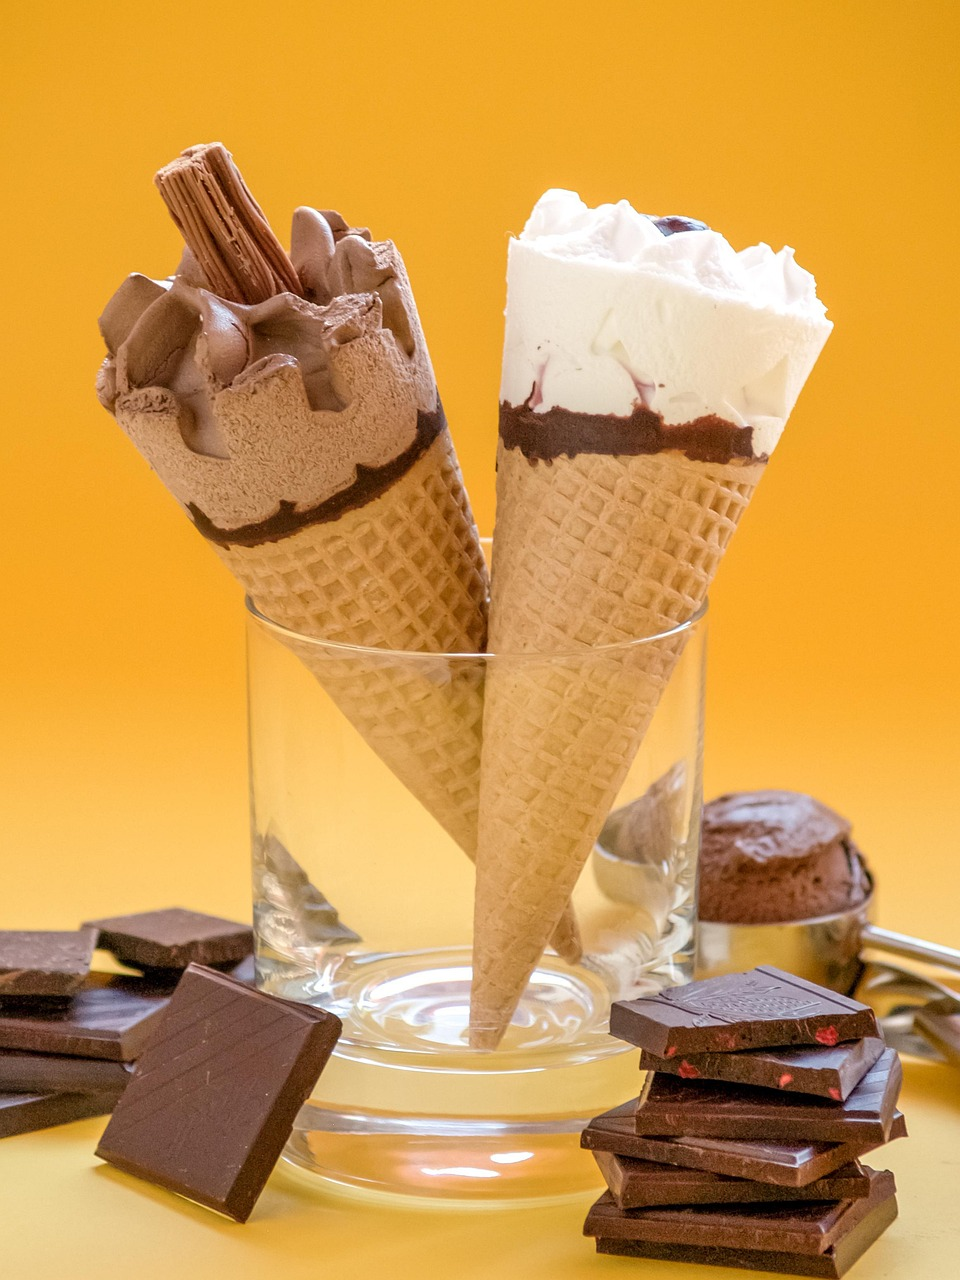
\includegraphics[width=4.0625in,height=\textheight]{book/img/ice-cream.jpg}

}

\caption{\label{fig-ice-cream}The two flavours of the ice cream cone you
sell across all your ice cream carts: \emph{vanilla} and
\emph{chocolate}. Image by
\href{https://pixabay.com/users/tomekwalecki-13027968/}{\emph{tomekwalecki}}
via
\href{https://pixabay.com/photos/ice-cream-flavor-chocolate-vanilla-4401300/}{\emph{Pixabay}}.}

\end{figure}%

Now, let us direct this whole case onto a more statistical and
probabilistic field; suppose you have a well-defined overall
\textcolor{blue}{population} of interest for those above eight Canadian
cities: \textbf{children between 4 and 11 years old attending these
parks during the Summer weekends}. Of course, Summer time is coming this
year, and you would like to know \textbf{which ice cream cone flavour is
the favourite one} for this \textcolor{blue}{population} (\emph{and by
how much!}). As a business owner, investigating ice cream flavour
preferences would allow you to plan Summer restocks more carefully with
your corresponding suppliers. Therefore, it would be essential to start
collecting consumer data so the company can tackle this \textbf{demand
query}.

Also, suppose there is a second query. For the sake of our case, we will
call it a \textbf{time query}. As a critical component of demand
planning, besides estimating which cone flavour is the most preferred
one (\emph{and by how much!}) for the above \textcolor{blue}{population}
of interest, the operations area is currently requiring a realistic
estimation of \textbf{the average waiting time from one customer to the
next one in any given cart during Summer weekends}. This average waiting
time would allow the operations team to plan carefully how much stock
each cart should have so there will not be any waste or shortage.

\begin{figure}[H]

{\centering 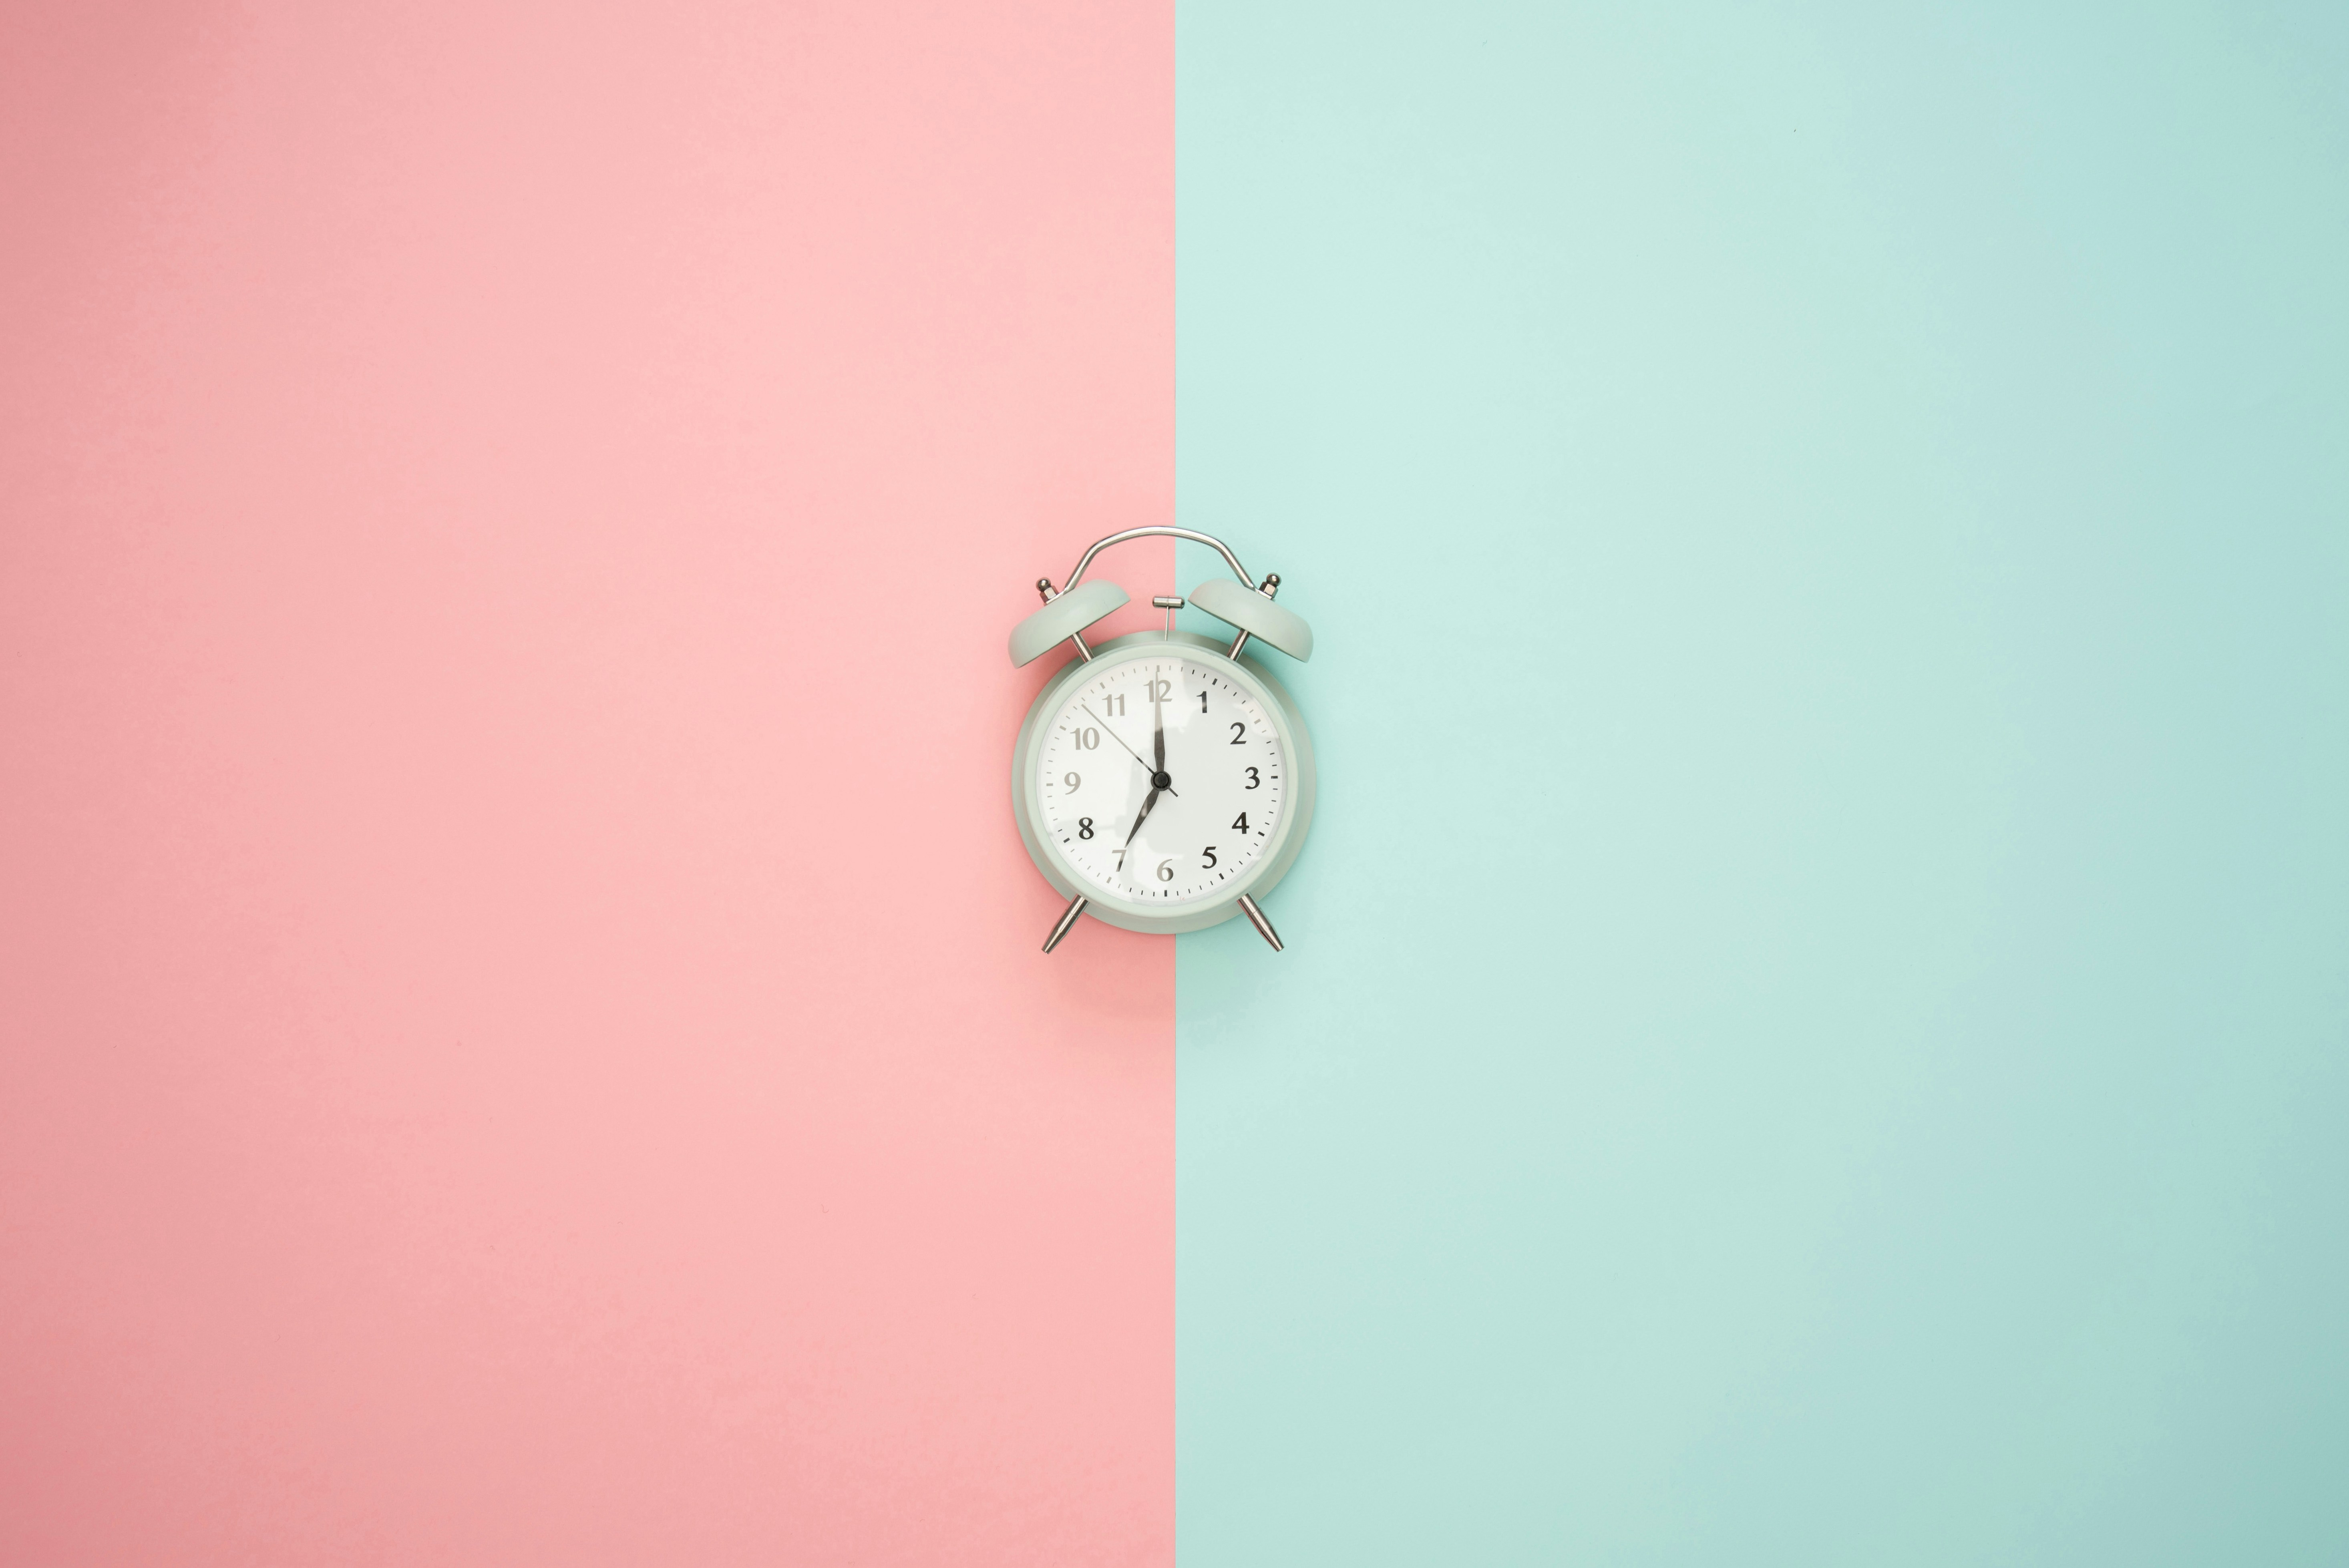
\includegraphics[width=5.20833in,height=\textheight]{book/img/clock.jpg}

}

\caption{Image by
\href{https://unsplash.com/@icons8?utm_content=creditCopyText&utm_medium=referral&utm_source=unsplash}{\emph{Icons8
Team}} via
\href{https://unsplash.com/photos/silver-bell-alarm-clock-dhZtNlvNE8M}{\emph{Unsplash}}.}

\end{figure}%

Note that the nature of the aforementioned \textbf{time query} is more
related to a larger \textcolor{blue}{population}. Therefore, we can
define it as \textbf{all our ice cream customers during the Summer
weekends}. Furthermore, this second definition would limit this query to
our corresponding general ice cream customers, given the requirements of
our operations team, and \textbf{not} all the children between 4 and 11
years old attending the parks during Summer weekends. Consequently, it
is crucial to note that the nature of our queries will dictate how we
define our \textcolor{blue}{population} and our subsequent data
modelling and statistical inference.

Summer time represents the most profitable season from a business
perspective, thus solving these above two queries is a significant
priority for your company. Hence, you decide to organize a meeting with
your eight general managers (one per Canadian city). Finally, during the
meeting with the general managers, it was decided to do the following:

\begin{enumerate}
\def\labelenumi{\arabic{enumi}.}
\tightlist
\item
  For the \textbf{demand query}, a comprehensive market study will be
  run on the \textcolor{blue}{population} of interest across the eight
  Canadian cities right before next Summer; suppose we are currently in
  Spring.
\item
  For the \textbf{time query}, since the operations team has not
  previously recorded any historical data, \textbf{ALL} vendor staff
  from 900 carts will start collecting data on \textbf{the waiting time
  in seconds} between each customer this upcoming Summer.
\end{enumerate}

Surprisingly, when discussing study requirements for the marketing firm
who would be in charge of it for the \textbf{demand query},
\emph{Vancouver's general manager} dares to state the following:

\begin{quote}
\emph{Since we're already planning to collect consumer data on these
cities, let's mimic a census-type study to ensure we can have the
\textbf{MOST PRECISE} results on their preferences.}
\end{quote}

On the other hand, when agreeing on the specific operations protocol to
start recording waiting times for all the 900 vending carts this
upcoming Summer, \emph{Ottawa's general manager} provides a comment for
further statistical food for thought:

\begin{quote}
\emph{The operations protocol for recording waiting times in the 900
vending carts looks too cumbersome to implement straightforwardly this
upcoming Summer. Why don't we select \textbf{A SMALLER GROUP} of ice
cream carts across the eight cities to have a more efficient process
implementation that would allow us to optimize operational costs?}
\end{quote}

Bingo! \emph{Ottawa's general manager} just nailed the probabilistic way
of making inference on our \textcolor{blue}{population parameter} of
interest for the \textbf{time query}. Indeed, their comment was
primarily framed from a business perspective of optimizing operational
costs. Still, this fact does not take away a crucial insight on which
statistical inference is built: a \textcolor{blue}{random sample} (as in
Important~\ref{imp-random-sample}). As for \emph{Vancouver's general
manager}, ironically, their statement is \textbf{NOT PRECISE} at all!
Mimicking a census-type study might not be the most optimal decision for
the \textbf{demand query} given the time constraint and the potential
size of its target \textcolor{blue}{population}.

\begin{quote}
\textbf{Realistically, there is no cheap and efficient way to conduct a
census-type study for any of the two queries!}
\end{quote}

We can state that \textcolor{blue}{probability} is viewed as the
language to decode random phenomena that occur in any given
\textcolor{blue}{population} or system of interest. In our example, we
have two random phenomena:

\begin{enumerate}
\def\labelenumi{\arabic{enumi}.}
\tightlist
\item
  For the \textbf{demand query}, a phenomenon can be represented by the
  preferred ice cream cone flavour of \textbf{any randomly selected
  child between 4 and 11 years old attending the parks of the above
  eight Canadian cities during the Summer weekends}.
\item
  Regarding the \textbf{time query}, a phenomenon of this kind can be
  represented by \textbf{any randomly recorded waiting time between two
  customers during a Summer weekend in any of the above eight Canadian
  cities}.
\end{enumerate}

Hence, let us finally define what we mean by
\textcolor{blue}{probability} along with the inherent concept of
\textcolor{blue}{sample space}.

\begin{figure}[H]

{\centering 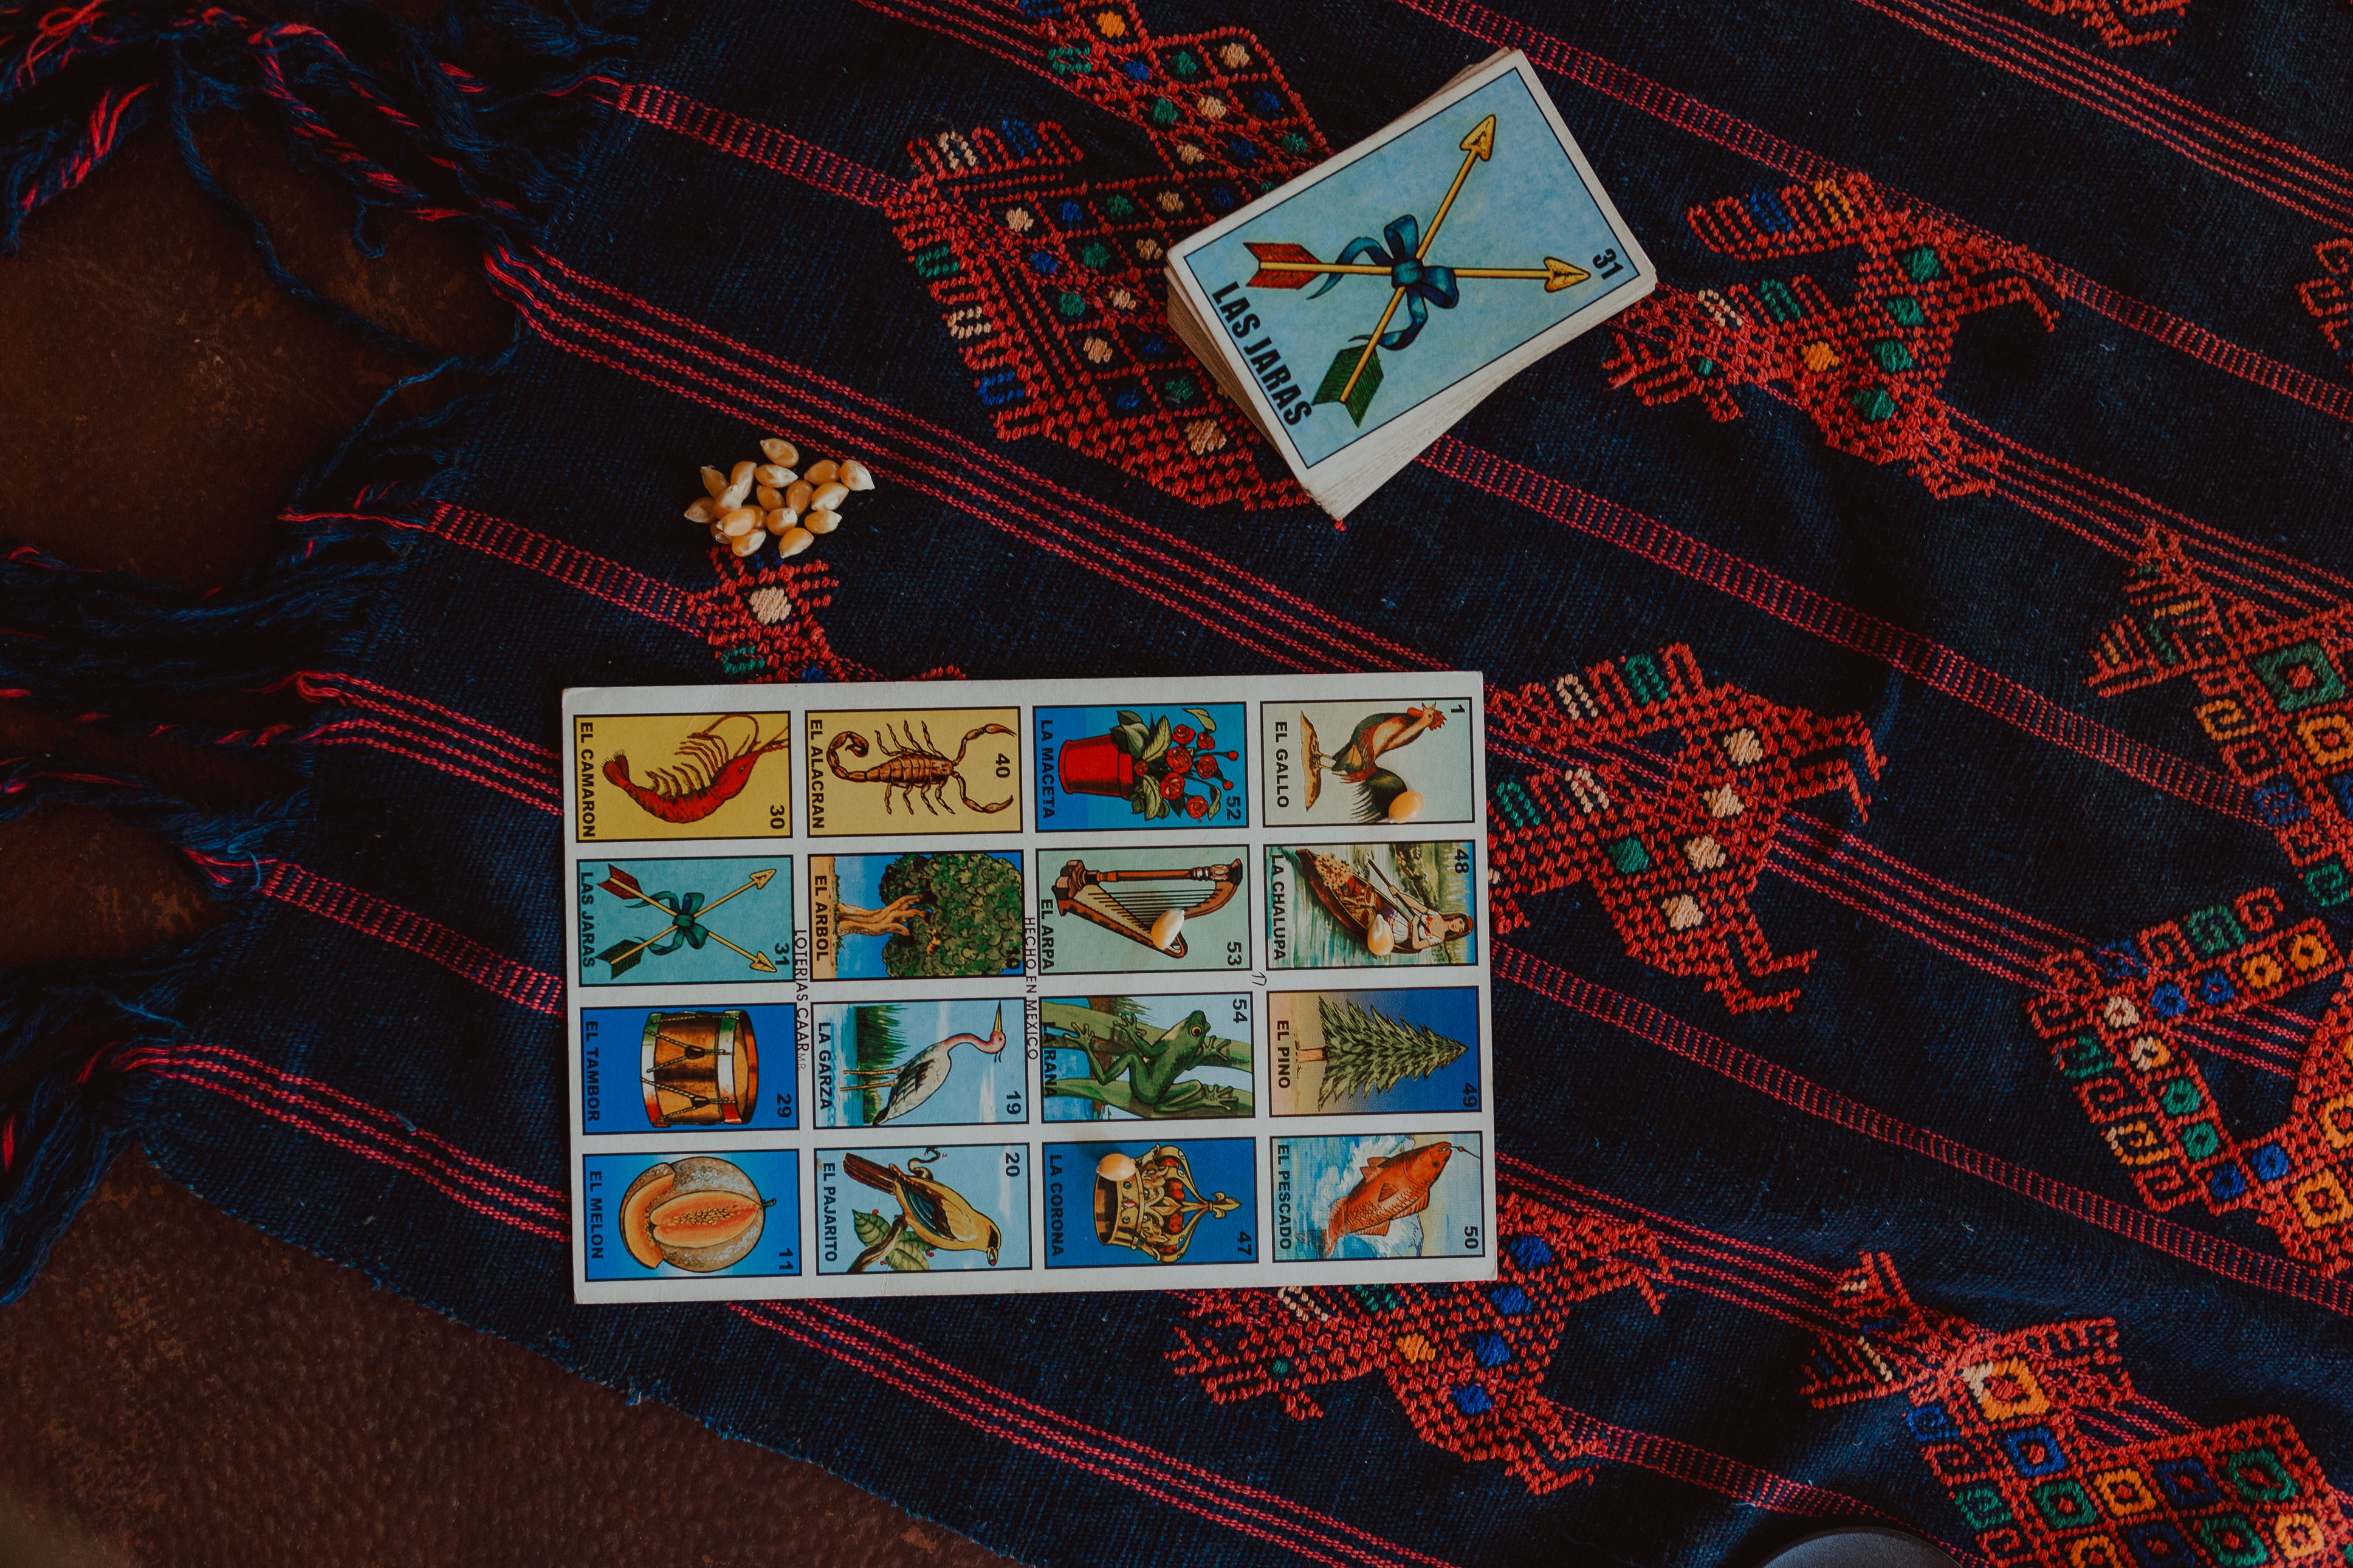
\includegraphics[width=5.72917in,height=\textheight]{book/img/loteria.jpg}

}

\caption{Mexican lotería, a bingo-type game. Image by
\href{https://unsplash.com/@irvinmac}{\emph{irvin Macfarland}} via
\href{https://unsplash.com/photos/blue-white-and-red-playing-cards-clelay10tfg}{\emph{Unsplash}}.}

\end{figure}%

\begin{tcolorbox}[enhanced jigsaw, bottomrule=.15mm, breakable, colback=white, leftrule=.75mm, coltitle=black, rightrule=.15mm, bottomtitle=1mm, title=\textcolor{quarto-callout-important-color}{\faExclamation}\hspace{0.5em}{Important \ref*{imp-probability}: Definition of probability}, opacitybacktitle=0.6, toprule=.15mm, titlerule=0mm, arc=.35mm, colbacktitle=quarto-callout-important-color!10!white, toptitle=1mm, colframe=quarto-callout-important-color-frame, left=2mm, opacityback=0]

\quartocalloutimp{imp-probability} 

Let \(A\) be an event of interest in a random phenomenon, in a
\textcolor{blue}{population} or \textbf{system} of interest, whose all
possible outcomes belong to a given \textcolor{blue}{sample space}
\(S\). Generally, the \textcolor{blue}{probability} for this event \(A\)
happening can be mathematically depicted as \(P(A)\). Moreover,
\textbf{suppose we observe the random phenomenon \(n\) times} such as we
were running some class of experiment, then \(P(A)\) is defined as the
following ratio:

\begin{equation}\phantomsection\label{eq-probability}{
P(A) = \frac{\text{Number of times event $A$ is observed}}{n},
}\end{equation}

\textbf{as the \(n\) times we observe the random phenomenon goes to
infinity.}\\

Equation~\ref{eq-probability} will always put \(P(A)\) in the following
numerical range:

\[
0 \leq P(A) \leq 1.
\]

\end{tcolorbox}

\begin{tcolorbox}[enhanced jigsaw, bottomrule=.15mm, breakable, colback=white, leftrule=.75mm, coltitle=black, rightrule=.15mm, bottomtitle=1mm, title=\textcolor{quarto-callout-important-color}{\faExclamation}\hspace{0.5em}{Important \ref*{imp-sample-space}: Definition of sample space}, opacitybacktitle=0.6, toprule=.15mm, titlerule=0mm, arc=.35mm, colbacktitle=quarto-callout-important-color!10!white, toptitle=1mm, colframe=quarto-callout-important-color-frame, left=2mm, opacityback=0]

\quartocalloutimp{imp-sample-space} 

Let \(A\) be an event of interest in a random phenomenon in a
\textcolor{blue}{population} or \textbf{system} of interest. The
\textcolor{blue}{sample space} \(S\) of event \(A\) denotes the set of
all the possible \textbf{random outcomes} we might encounter every time
we randomly observe \(A\) such as we were running some class of
experiment.\\

Note each of these outcomes has a determined probability associated with
them. If we add up all these probabilities, the probability of the
sample \(S\) will be one, i.e.,

\begin{equation}\phantomsection\label{eq-sample-space}{
P(S) = 1.
}\end{equation}

\end{tcolorbox}

Note the definition of the \textcolor{blue}{probability} for an event
\(A\) in Important~\ref{imp-probability} specifically highlights the
following:

\begin{quote}
\textbf{\ldots{} as the \(n\) times we observe the random phenomenon
goes to infinity.}
\end{quote}

The ``\emph{infinity}'' term is key when it comes to an understanding
the philosophy behind the \textcolor{blue}{frequentist} school of
statistical thinking in contrast to its \textcolor{blue}{Bayesian}
counterpart. In general, the \textcolor{blue}{frequentist} way of
practicing statistics in terms of \textcolor{blue}{probability} and
inference is the approach we usually learn in introductory courses, more
specifically when it comes to \textcolor{blue}{hypothesis testing} and
\textcolor{blue}{confidence intervals} which will be explored in
Section~\ref{sec-basics-inf}. That said, the Bayesian approach is
another way of practicing statistical inference. Its philosophy differs
in what information is used to infer our
\textcolor{blue}{population parameters} of interest. Below, we briefly
define both schools of thinking.

\begin{tcolorbox}[enhanced jigsaw, bottomrule=.15mm, breakable, colback=white, leftrule=.75mm, coltitle=black, rightrule=.15mm, bottomtitle=1mm, title=\textcolor{quarto-callout-important-color}{\faExclamation}\hspace{0.5em}{Important \ref*{imp-frequentist-stats}: Definition of frequentist statistics}, opacitybacktitle=0.6, toprule=.15mm, titlerule=0mm, arc=.35mm, colbacktitle=quarto-callout-important-color!10!white, toptitle=1mm, colframe=quarto-callout-important-color-frame, left=2mm, opacityback=0]

\quartocalloutimp{imp-frequentist-stats} 

This statistical school of thinking heavily relies on the
\textbf{frequency of events} to estimate specific
\textcolor{blue}{parameters} of interest in a
\textcolor{blue}{population} or \textbf{system}. This frequency of
events is reflected in the repetition of \(n\) experiments involving a
random phenomenon within this \textcolor{blue}{population} or
\textbf{system}.\\

Under the umbrella of this approach, we assume that our governing
\textcolor{blue}{parameters} are \textbf{fixed}. Note that, within the
philosophy of this school of thinking, we can only make \textbf{precise}
and \textbf{accurate} predictions as long as we repeat our \(n\)
experiments as many times as possible, i.e.,

\[
n \rightarrow \infty.
\]

\begin{figure}[H]

{\centering 
\includegraphics[width=4.16667in,height=\textheight]{book/img/infinity.jpg}

}

\caption{Image by
\href{https://pixabay.com/users/maricarmennd9-3511650/?utm_source=link-attribution&utm_medium=referral&utm_campaign=image&utm_content=1737624}{\emph{Mari
Carmen Díaz}} via
\href{https://pixabay.com//?utm_source=link-attribution&utm_medium=referral&utm_campaign=image&utm_content=1737624}{\emph{Pixabay}}.}

\end{figure}%

\end{tcolorbox}

\begin{tcolorbox}[enhanced jigsaw, bottomrule=.15mm, breakable, colback=white, leftrule=.75mm, coltitle=black, rightrule=.15mm, bottomtitle=1mm, title=\textcolor{quarto-callout-important-color}{\faExclamation}\hspace{0.5em}{Important \ref*{imp-bayesian-stats}: Definition of Bayesian statistics}, opacitybacktitle=0.6, toprule=.15mm, titlerule=0mm, arc=.35mm, colbacktitle=quarto-callout-important-color!10!white, toptitle=1mm, colframe=quarto-callout-important-color-frame, left=2mm, opacityback=0]

\quartocalloutimp{imp-bayesian-stats} 

This statistical school of thinking also relies on the \textbf{frequency
of events} to estimate specific \textcolor{blue}{parameters} of interest
in a \textcolor{blue}{population} or \textbf{system}. Nevertheless,
unlike \textcolor{blue}{frequentist} statistics,
\textcolor{blue}{Bayesian} statisticians use \textbf{prior knowledge} on
the \textcolor{blue}{population parameters} to update their estimations
on them along with the \textbf{current evidence} they can gather. This
evidence is in the form of the repetition of \(n\) experiments involving
a random phenomenon. All these ingredients allow
\textcolor{blue}{Bayesian} statisticians to make inference by conducting
appropriate \textcolor{blue}{hypothesis testings}, which are designed
differently from their mainstream \textcolor{blue}{frequentist}
counterpart.\\

\begin{figure}[H]

{\centering 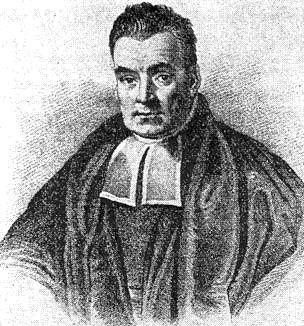
\includegraphics[width=3.125in,height=\textheight]{book/img/thomas-bayes.jpg}

}

\caption{The unique known portrait of Reverend Thomas Bayes according to
O'Donnell, T. (1936), even though Bellhouse (2004) argues it might not
be a Bayes' portrait.}

\end{figure}%

Under the umbrella of this approach, we assume that our governing
\textcolor{blue}{parameters} are \textbf{random}; i.e., they have their
own \textcolor{blue}{sample space} and \textcolor{blue}{probabilities}
associated to their corresponding outcomes. The statistical process of
inference is heavily backed up by \textbf{probability theory} mostly in
the form of the \textbf{Bayes theorem} (named after Reverend
\textbf{Thomas Bayes}, an English statistician from the 18th century).
This theorem uses our \textbf{current evidence} along with our
\textbf{prior beliefs} to deliver a \textbf{posterior distribution} of
our \textbf{random} \textcolor{blue}{parameter(s)} of interest.

\end{tcolorbox}

Let us put the definitions for both schools from
Important~\ref{imp-frequentist-stats} and
Important~\ref{imp-bayesian-stats} into a more concrete example. We can
use the \textbf{demand query} from our ice cream case as a starting
point. More concretely, we can dig more into a standalone
\textcolor{blue}{population parameter} such as the probability that a
randomly selected child between 4 and 11 years old, attending the parks
of the above eight Canadian cities during the Summer weekends, prefers
the chocolate-flavoured ice cream cone over the vanilla one. Think about
the following two hypothetical questions:

\begin{enumerate}
\def\labelenumi{\alph{enumi}.}
\tightlist
\item
  From a \textcolor{blue}{frequentist} point of view, what is the
  \textbf{estimated} \textcolor{blue}{probability} of \textbf{preferring
  chocolate over vanilla} after \textbf{randomly} surveying \(n = 100\)
  children from our \textcolor{blue}{population} of interest?
\item
  Using a \textcolor{blue}{Bayesian} approach, suppose the marketing
  team has found ten \textbf{prior} market studies on similar children
  \textcolor{blue}{populations} on their preferred ice cream flavour
  (between chocolate and vanilla). Therefore, along with our actual
  \textbf{random} survey of \(n = 100\) children from our
  \textcolor{blue}{population} of interest, what is the
  \textbf{posterior estimation} of the \textcolor{blue}{probability} of
  \textbf{preferring chocolate over vanilla}?
\end{enumerate}

\begin{tcolorbox}[enhanced jigsaw, bottomrule=.15mm, breakable, colback=white, leftrule=.75mm, coltitle=black, rightrule=.15mm, bottomtitle=1mm, title=\textcolor{quarto-callout-note-color}{\faInfo}\hspace{0.5em}{Note \ref*{nte-frequentist-and-bayesian}: Heads-up on the difference between frequentist and Bayesian statistics!}, opacitybacktitle=0.6, toprule=.15mm, titlerule=0mm, arc=.35mm, colbacktitle=quarto-callout-note-color!10!white, toptitle=1mm, colframe=quarto-callout-note-color-frame, left=2mm, opacityback=0]

\quartocalloutnte{nte-frequentist-and-bayesian} 

\end{tcolorbox}

Equation~\ref{eq-bernoulli-pmf}

\begin{equation}\phantomsection\label{eq-bernoulli-pmf}{
P(X = x \mid \pi) = \pi^x (1 - \pi)^{1 - x} \quad \text{for} \quad x = 0, 1.
}\end{equation}

\begin{tcolorbox}[enhanced jigsaw, bottomrule=.15mm, breakable, colback=white, leftrule=.75mm, coltitle=black, rightrule=.15mm, bottomtitle=1mm, title=\textcolor{quarto-callout-important-color}{\faExclamation}\hspace{0.5em}{Important \ref*{imp-random-sample}: Definition of random sample}, opacitybacktitle=0.6, toprule=.15mm, titlerule=0mm, arc=.35mm, colbacktitle=quarto-callout-important-color!10!white, toptitle=1mm, colframe=quarto-callout-important-color-frame, left=2mm, opacityback=0]

\quartocalloutimp{imp-random-sample} 

\end{tcolorbox}

\section{What is Maximum Likelihood Estimation?}\label{sec-mle}

\section{Basics of Frequentist Statistical
Inference}\label{sec-basics-inf}

\section{Supervised Learning and Regression
Analysis}\label{sec-sup-learning-regression}

\bookmarksetup{startatroot}

\chapter{Ordinary Least-squares}\label{sec-ols}

\bookmarksetup{startatroot}

\chapter*{References}\label{references}
\addcontentsline{toc}{chapter}{References}

\markboth{References}{References}

\phantomsection\label{refs}
\begin{CSLReferences}{1}{0}
\bibitem[\citeproctext]{ref-bellhouse2004}
Bellhouse, D. R. 2004. {``{The Reverend Thomas Bayes, FRS: A Biography
to Celebrate the Tercentenary of His Birth}.''} \emph{Statistical
Science} 19 (1): 3--43.
\url{https://doi.org/10.1214/088342304000000189}.

\bibitem[\citeproctext]{ref-gelbart2017}
Gelbart, Michael. 2017. {``Data Science Terminology.''} \emph{UBC MDS}.
Master of Data Science at the University of British Columbia.
\url{https://ubc-mds.github.io/resources_pages/terminology/}.

\bibitem[\citeproctext]{ref-odonnell1936}
O'Donnell, T. 1936. \emph{{History of Life Insurance in Its Formative
Years. Compiled from Approved Sources by T. O'Donnell}}. Chicago.

\bibitem[\citeproctext]{ref-r2024}
R Core Team. 2024. {``R: A Language and Environment for Statistical
Computing.''} Vienna, Austria: R Foundation for Statistical Computing.
\url{https://www.R-project.org/}.

\bibitem[\citeproctext]{ref-pandas2024}
The Pandas Development Team. 2024. {``Pandas-Dev/Pandas: Pandas.''}
Zenodo. \url{https://doi.org/10.5281/zenodo.3509134}.

\bibitem[\citeproctext]{ref-python}
Van Rossum, Guido, and Fred L. Drake. 2009. \emph{Python 3 Reference
Manual}. Scotts Valley, CA: CreateSpace.

\bibitem[\citeproctext]{ref-tidyverse}
Wickham, Hadley, Mara Averick, Jennifer Bryan, Winston Chang, Lucy
D'Agostino McGowan, Romain François, Garrett Grolemund, et al. 2019.
{``Welcome to the {tidyverse}.''} \emph{Journal of Open Source Software}
4 (43): 1686. \url{https://doi.org/10.21105/joss.01686}.

\end{CSLReferences}

\cleardoublepage
\phantomsection
\addcontentsline{toc}{part}{Appendices}
\appendix

\chapter{The ML-Stats Dictionary}\label{sec-dictionary}

Machine learning and statistics comprise a \textbf{substantial synergy}
that is reflected in data science. Thus, it is imperative to construct
solid bridges between both disciplines to ensure everything is clear
regarding their tremendous amount of jargon and terminology. This
\textbf{ML-Stats dictionary} (\emph{ML} stands for \emph{Machine
Learning}) aims to be one of these bridges in this textbook, especially
within supervised learning and regression analysis contexts.

\begin{figure}[H]

{\centering \includegraphics[width=5.72917in,height=\textheight]{book/img/definition.jpg}

}

\caption{Image by
\href{https://pixabay.com/users/geralt-9301/}{\emph{Gerd Altmann}} via
\href{https://pixabay.com/photos/definition-books-library-bookshelf-4255486/}{\emph{Pixabay}}.}

\end{figure}%

Below, you will find definitions either highlighted in
\textcolor{blue}{blue} if they correspond to
\textcolor{blue}{statistical} terminology or
\textcolor{magenta}{magenta} if the terminology is
\textcolor{magenta}{machine learning-related}. These definitions come
from all \textbf{definition} admonitions, such as in
\textbf{?@imp-example}. This colour scheme strives to combine all
terminology to switch from one field to another easily. With practice
and time, we should be able to jump back and forth when using these
concepts.

\begin{tcolorbox}[enhanced jigsaw, bottomrule=.15mm, breakable, colback=white, leftrule=.75mm, coltitle=black, rightrule=.15mm, bottomtitle=1mm, title=\textcolor{quarto-callout-warning-color}{\faExclamationTriangle}\hspace{0.5em}{Attention!}, opacitybacktitle=0.6, toprule=.15mm, titlerule=0mm, arc=.35mm, colbacktitle=quarto-callout-warning-color!10!white, toptitle=1mm, colframe=quarto-callout-warning-color-frame, left=2mm, opacityback=0]

Noteworthy terms (either \textcolor{blue}{statistical} or
\textcolor{magenta}{machine learning-related}) will include a particular
admonition identifying which terms (again, either
\textcolor{blue}{statistical} or
\textcolor{magenta}{machine learning-related}) are \textbf{equivalent}
(\textbf{or NOT equivalent if that is the case!}).

\end{tcolorbox}

\section*{B}\label{b}
\addcontentsline{toc}{section}{B}

\markright{B}

\subsection*{\texorpdfstring{\textcolor{blue}{Bayesian statistics}}{}}\label{section}
\addcontentsline{toc}{subsection}{\textcolor{blue}{Bayesian statistics}}

This statistical school of thinking also relies on the \textbf{frequency
of events} to estimate specific \textcolor{blue}{parameters} of interest
in a \textcolor{blue}{population} or \textbf{system}. Nevertheless,
unlike \textcolor{blue}{frequentist} statistics,
\textcolor{blue}{Bayesian} statisticians use \textbf{prior knowledge} on
the \textcolor{blue}{population parameters} to update their estimations
on them along with the \textbf{current evidence} they can gather. This
evidence is in the form of the repetition of \(n\) experiments involving
a random phenomenon. All these ingredients allow
\textcolor{blue}{Bayesian} statisticians to make inference by conducting
appropriate \textcolor{blue}{hypothesis testings}, which are designed
differently from their mainstream \textcolor{blue}{frequentist}
counterpart.

Under the umbrella of this approach, we assume that our governing
\textcolor{blue}{parameters} are \textbf{random}; i.e., they have their
own \textcolor{blue}{sample space} and \textcolor{blue}{probabilities}
associated to their corresponding outcomes. The statistical process of
inference is heavily backed up by \textbf{probability theory} mostly in
the form of the \textbf{Bayes theorem} (named after Reverend
\textbf{Thomas Bayes}, an English statistician from the 18th century).
This theorem uses our \textbf{current evidence} along with our
\textbf{prior beliefs} to deliver a \textbf{posterior distribution} of
our \textbf{random} \textcolor{blue}{parameter(s)} of interest.

\section*{D}\label{d}
\addcontentsline{toc}{section}{D}

\markright{D}

\subsection*{\texorpdfstring{\textcolor{blue}{Dependent variable}}{}}\label{section-1}
\addcontentsline{toc}{subsection}{\textcolor{blue}{Dependent variable}}

In supervised learning, it is the main variable of interest we are
trying to \textbf{learn} or \textbf{predict}, or equivalently, the
variable we are trying \textbf{explain} in a statistical inference
framework.

\begin{tcolorbox}[enhanced jigsaw, bottomrule=.15mm, breakable, colback=white, leftrule=.75mm, coltitle=black, rightrule=.15mm, bottomtitle=1mm, title=\textcolor{quarto-callout-warning-color}{\faExclamationTriangle}\hspace{0.5em}{Equivalent to:}, opacitybacktitle=0.6, toprule=.15mm, titlerule=0mm, arc=.35mm, colbacktitle=quarto-callout-warning-color!10!white, toptitle=1mm, colframe=quarto-callout-warning-color-frame, left=2mm, opacityback=0]

\textcolor{blue}{Response}, \textcolor{magenta}{outcome},
\textcolor{magenta}{output} or \textcolor{magenta}{target}.

\end{tcolorbox}

\section*{F}\label{f}
\addcontentsline{toc}{section}{F}

\markright{F}

\subsection*{\texorpdfstring{\textcolor{blue}{Frequentist statistics}}{}}\label{section-2}
\addcontentsline{toc}{subsection}{\textcolor{blue}{Frequentist statistics}}

This statistical school of thinking heavily relies on the
\textbf{frequency of events} to estimate specific
\textcolor{blue}{parameters} of interest in a
\textcolor{blue}{population} or \textbf{system}. This frequency of
events is reflected in the repetition of \(n\) experiments involving a
random phenomenon within this \textcolor{blue}{population} or
\textbf{system}.\\

Under the umbrella of this approach, we assume that our governing
\textcolor{blue}{parameters} are \textbf{fixed}. Note that, within the
philosophy of this school of thinking, we can only make \textbf{precise}
and \textbf{accurate} predictions as long as we repeat our \(n\)
experiments as many times as possible, i.e.,

\[
n \rightarrow \infty.
\]

\section*{O}\label{o}
\addcontentsline{toc}{section}{O}

\markright{O}

\subsection*{\texorpdfstring{\textcolor{magenta}{Outcome}}{}}\label{section-3}
\addcontentsline{toc}{subsection}{\textcolor{magenta}{Outcome}}

In supervised learning, it is the main variable of interest we are
trying to \textbf{learn} or \textbf{predict}, or equivalently, the
variable we are trying \textbf{explain} in a statistical inference
framework.

\begin{tcolorbox}[enhanced jigsaw, bottomrule=.15mm, breakable, colback=white, leftrule=.75mm, coltitle=black, rightrule=.15mm, bottomtitle=1mm, title=\textcolor{quarto-callout-warning-color}{\faExclamationTriangle}\hspace{0.5em}{Equivalent to:}, opacitybacktitle=0.6, toprule=.15mm, titlerule=0mm, arc=.35mm, colbacktitle=quarto-callout-warning-color!10!white, toptitle=1mm, colframe=quarto-callout-warning-color-frame, left=2mm, opacityback=0]

\textcolor{blue}{Dependent variable}, \textcolor{blue}{response},
\textcolor{magenta}{output} or \textcolor{magenta}{target}.

\end{tcolorbox}

\subsection*{\texorpdfstring{\textcolor{magenta}{Output}}{}}\label{section-4}
\addcontentsline{toc}{subsection}{\textcolor{magenta}{Output}}

In supervised learning, it is the main variable of interest we are
trying to \textbf{learn} or \textbf{predict}, or equivalently, the
variable we are trying \textbf{explain} in a statistical inference
framework.

\begin{tcolorbox}[enhanced jigsaw, bottomrule=.15mm, breakable, colback=white, leftrule=.75mm, coltitle=black, rightrule=.15mm, bottomtitle=1mm, title=\textcolor{quarto-callout-warning-color}{\faExclamationTriangle}\hspace{0.5em}{Equivalent to:}, opacitybacktitle=0.6, toprule=.15mm, titlerule=0mm, arc=.35mm, colbacktitle=quarto-callout-warning-color!10!white, toptitle=1mm, colframe=quarto-callout-warning-color-frame, left=2mm, opacityback=0]

\textcolor{blue}{Dependent variable}, \textcolor{blue}{response},
\textcolor{magenta}{outcome} or \textcolor{magenta}{target}.

\end{tcolorbox}

\section*{P}\label{p}
\addcontentsline{toc}{section}{P}

\markright{P}

\subsection*{\texorpdfstring{\textcolor{blue}{Parameter}}{}}\label{section-5}
\addcontentsline{toc}{subsection}{\textcolor{blue}{Parameter}}

It is a characteristic (\textbf{numerical} or even
\textbf{non-numerical}, such as a \textbf{distinctive category}) that
\textbf{summarizes} the state of our \textcolor{blue}{population} or
\textbf{system} of interest. Examples of a
\textcolor{blue}{population parameter} can be described as follows:

\begin{itemize}
\tightlist
\item
  \emph{The average weight of children between the ages of 5 and 10
  years old in states of the American west coast (\textbf{numerical}).}
\item
  \emph{The variability in the height of the mature açaí palm trees from
  the Brazilian Amazonian jungle (\textbf{numerical}).}
\item
  \emph{The proportion of defective items in the production of cellular
  phones in a set of manufacturing facilities (\textbf{numerical}).}
\item
  \emph{The average customer waiting time to get their order in the
  Vancouver franchises of a well-known ice cream parlour
  (\textbf{numerical}).}
\item
  \emph{The most favourite pizza topping of vegetarian adults between
  the ages of 30 and 40 years old in Edmonton (\textbf{non-numerical}).}
\end{itemize}

Note the \textbf{standard mathematical notation} for
\textcolor{blue}{population parameters} are \textbf{Greek letters}.
Moreover, in practice, these \textcolor{blue}{population parameter(s)}
of interest will be \textbf{unknown} to the data scientist or
researcher. Instead, they would use formal statistical inference to
\textbf{estimate} them.

\subsection*{\texorpdfstring{\textcolor{blue}{Population}}{}}\label{section-6}
\addcontentsline{toc}{subsection}{\textcolor{blue}{Population}}

It is a \textbf{whole collection of individuals or items} that share
\textbf{distinctive attributes}. As data scientists or researchers, we
are interested in studying these attributes, which we assume are
\textbf{governed} by \textcolor{blue}{parameters}. In practice, we must
be \textbf{as precise as possible} when defining our given
\textcolor{blue}{population} such that we would frame our entire data
modelling process since its very early stages. Examples of a
\textcolor{blue}{population} could be the following:

\begin{itemize}
\tightlist
\item
  \emph{Children between the ages of 5 and 10 years old in states of the
  American west coast.}
\item
  \emph{Customers of musical vinyl records in the Canadian provinces of
  British Columbia and Alberta.}
\item
  \emph{Avocado trees grown in the Mexican state of Michoacán.}
\item
  \emph{Adult giant pandas in the Southwestern Chinese province of
  Sichuan.}
\item
  \emph{Mature açaí palm trees from the Brazilian Amazonian jungle.}
\end{itemize}

Note that the term \textcolor{blue}{population} could be exchanged for
the term \textbf{system}, given that certain contexts do not
specifically refer to individuals or items. Instead, these contexts
could refer to \textbf{processes} whose attributes are also governed by
\textcolor{blue}{parameters}. Examples of a \textbf{system} could be the
following:

\begin{itemize}
\tightlist
\item
  \emph{The production of cellular phones in a set of manufacturing
  facilities.}
\item
  \emph{The sale process in the Vancouver franchises of a well-known ice
  cream parlour.}
\item
  \emph{The transit cycle of the twelve lines of Mexico City's subway.}
\end{itemize}

\subsection*{\texorpdfstring{\textcolor{blue}{Probability}}{}}\label{section-7}
\addcontentsline{toc}{subsection}{\textcolor{blue}{Probability}}

Let \(A\) be an event of interest in a random phenomenon, in a
\textcolor{blue}{population} or \textbf{system} of interest, whose all
possible outcomes belong to a given \textcolor{blue}{sample space}
\(S\). Generally, the \textcolor{blue}{probability} for this event \(A\)
happening can be mathematically depicted as \(P(A)\). Moreover,
\textbf{suppose we observe the random phenomenon \(n\) times} such as we
were running some class of experiment, then \(P(A)\) is defined as the
following ratio:

\begin{equation}\phantomsection\label{eq-probability-dictionary}{
P(A) = \frac{\text{Number of times event $A$ is observed}}{n},
}\end{equation}

\textbf{as the \(n\) times we observe the random phenomenon goes to
infinity.}

Equation~\ref{eq-probability-dictionary} will always put \(P(A)\) in the
following numerical range:

\[
0 \leq P(A) \leq 1.
\]

\section*{R}\label{r}
\addcontentsline{toc}{section}{R}

\markright{R}

\subsection*{\texorpdfstring{\textcolor{blue}{Response}}{}}\label{section-8}
\addcontentsline{toc}{subsection}{\textcolor{blue}{Response}}

In supervised learning, it is the main variable of interest we are
trying to \textbf{learn} or \textbf{predict}, or equivalently, the
variable we are trying \textbf{explain} in a statistical inference
framework.

\begin{tcolorbox}[enhanced jigsaw, bottomrule=.15mm, breakable, colback=white, leftrule=.75mm, coltitle=black, rightrule=.15mm, bottomtitle=1mm, title=\textcolor{quarto-callout-warning-color}{\faExclamationTriangle}\hspace{0.5em}{Equivalent to:}, opacitybacktitle=0.6, toprule=.15mm, titlerule=0mm, arc=.35mm, colbacktitle=quarto-callout-warning-color!10!white, toptitle=1mm, colframe=quarto-callout-warning-color-frame, left=2mm, opacityback=0]

\textcolor{blue}{Dependent variable}, \textcolor{magenta}{outcome},
\textcolor{magenta}{output} or \textcolor{magenta}{target}.

\end{tcolorbox}

\section*{S}\label{s}
\addcontentsline{toc}{section}{S}

\markright{S}

\subsection*{\texorpdfstring{\textcolor{blue}{Sample space}}{}}\label{section-9}
\addcontentsline{toc}{subsection}{\textcolor{blue}{Sample space}}

Let \(A\) be an event of interest in a random phenomenon in a
\textcolor{blue}{population} or \textbf{system} of interest. The
\textcolor{blue}{sample space} \(S\) of event \(A\) denotes the set of
all the possible \textbf{random outcomes} we might encounter every time
we randomly observe \(A\) such as we were running some class of
experiment.

Note each of these outcomes has a determined probability associated with
them. If we add up all these probabilities, the probability of the
sample \(S\) will be one, i.e.,

\begin{equation}\phantomsection\label{eq-sample-space}{
P(S) = 1.
}\end{equation}

\section*{T}\label{t}
\addcontentsline{toc}{section}{T}

\markright{T}

\subsection*{\texorpdfstring{\textcolor{magenta}{Target}}{}}\label{section-10}
\addcontentsline{toc}{subsection}{\textcolor{magenta}{Target}}

In supervised learning, it is the main variable of interest we are
trying to \textbf{learn} or \textbf{predict}, or equivalently, the
variable we are trying \textbf{explain} in a statistical inference
framework.

\begin{tcolorbox}[enhanced jigsaw, bottomrule=.15mm, breakable, colback=white, leftrule=.75mm, coltitle=black, rightrule=.15mm, bottomtitle=1mm, title=\textcolor{quarto-callout-warning-color}{\faExclamationTriangle}\hspace{0.5em}{Equivalent to:}, opacitybacktitle=0.6, toprule=.15mm, titlerule=0mm, arc=.35mm, colbacktitle=quarto-callout-warning-color!10!white, toptitle=1mm, colframe=quarto-callout-warning-color-frame, left=2mm, opacityback=0]

\textcolor{blue}{Dependent variable}, \textcolor{blue}{response},
\textcolor{magenta}{outcome} or \textcolor{magenta}{output}.

\end{tcolorbox}

\chapter{Greek Alphabet}\label{sec-greek-alphabet}

\textbf{Statistical notation} can be pretty particular and different
from \textbf{usual mathematical notation}. One of these particularities
is the constant use of \textbf{Greek letters} to denote unknown
\textcolor{blue}{population parameters} in \textbf{modelling setup},
\textbf{estimation}, and \textbf{statistical inference}. In that spirit,
throughout this book, we use diverse Greek letters to denote our
regression \textcolor{blue}{parameters} across each of the outlined
models in every chapter.

\begin{figure}[H]

{\centering \includegraphics[width=5.20833in,height=\textheight]{book/img/typewriter.jpg}

}

\caption{Image by
\href{https://pixabay.com/users/meineresterampe-26089/}{\emph{meineresterampe}}
via
\href{https://pixabay.com/photos/typewriter-old-retro-office-1899760/}{\emph{Pixabay}}.}

\end{figure}%

During early learning stages of regression modelling, we may feel
overwhelmed by these new letters, which could be unfamiliar. Therefore,
whenever confusion arises in any of the main chapters in this book
regarding the names of these letters, we recommend checking out the
Greek alphabet from table Table~\ref{tbl-greek-alphabet}. Note that
\textcolor{blue}{frequentist} statistical inference mostly uses
lowercase letters. \textbf{With practice over time, you would likely end
up memorizing most of this alphabet.}

\begin{longtable}[]{@{}ccc@{}}
\caption{Greek alphabet composed of 24 letters, from \emph{left} to
\emph{right} you can find the \emph{name} of letter along with its
corresponding \emph{uppercase} and \emph{lowercase}
forms.}\label{tbl-greek-alphabet}\tabularnewline
\toprule\noalign{}
Name & Uppercase & Lowercase \\
\midrule\noalign{}
\endfirsthead
\toprule\noalign{}
Name & Uppercase & Lowercase \\
\midrule\noalign{}
\endhead
\bottomrule\noalign{}
\endlastfoot
Alpha & \(\text{A}\) & \(\alpha\) \\
Beta & \(\text{B}\) & \(\beta\) \\
Gamma & \(\Gamma\) & \(\gamma\) \\
Delta & \(\Delta\) & \(\delta\) \\
Epsilon & \(\text{E}\) & \(\epsilon\) \\
Zeta & \(\text{Z}\) & \(\zeta\) \\
Eta & \(\text{H}\) & \(\eta\) \\
Theta & \(\Theta\) & \(\theta\) \\
Iota & \(\text{I}\) & \(\iota\) \\
Kappa & \(\text{K}\) & \(\kappa\) \\
Lambda & \(\Lambda\) & \(\lambda\) \\
Mu & \(\text{M}\) & \(\mu\) \\
Nu & \(\text{N}\) & \(\nu\) \\
Xi & \(\Xi\) & \(\xi\) \\
O & \(\text{O}\) & \(\text{o}\) \\
Pi & \(\Pi\) & \(\pi\) \\
Rho & \(\text{P}\) & \(\rho\) \\
Sigma & \(\Sigma\) & \(\sigma\) \\
Tau & \(\text{T}\) & \(\tau\) \\
Upsilon & \(\Upsilon\) & \(\upsilon\) \\
Phi & \(\Phi\) & \(\phi\) \\
Chi & \(\text{X}\) & \(\chi\) \\
Psi & \(\Psi\) & \(\psi\) \\
Omega & \(\Omega\) & \(\omega\) \\
\end{longtable}

\chapter{Distributional Cheatsheet}\label{sec-distributional-cheatsheet}

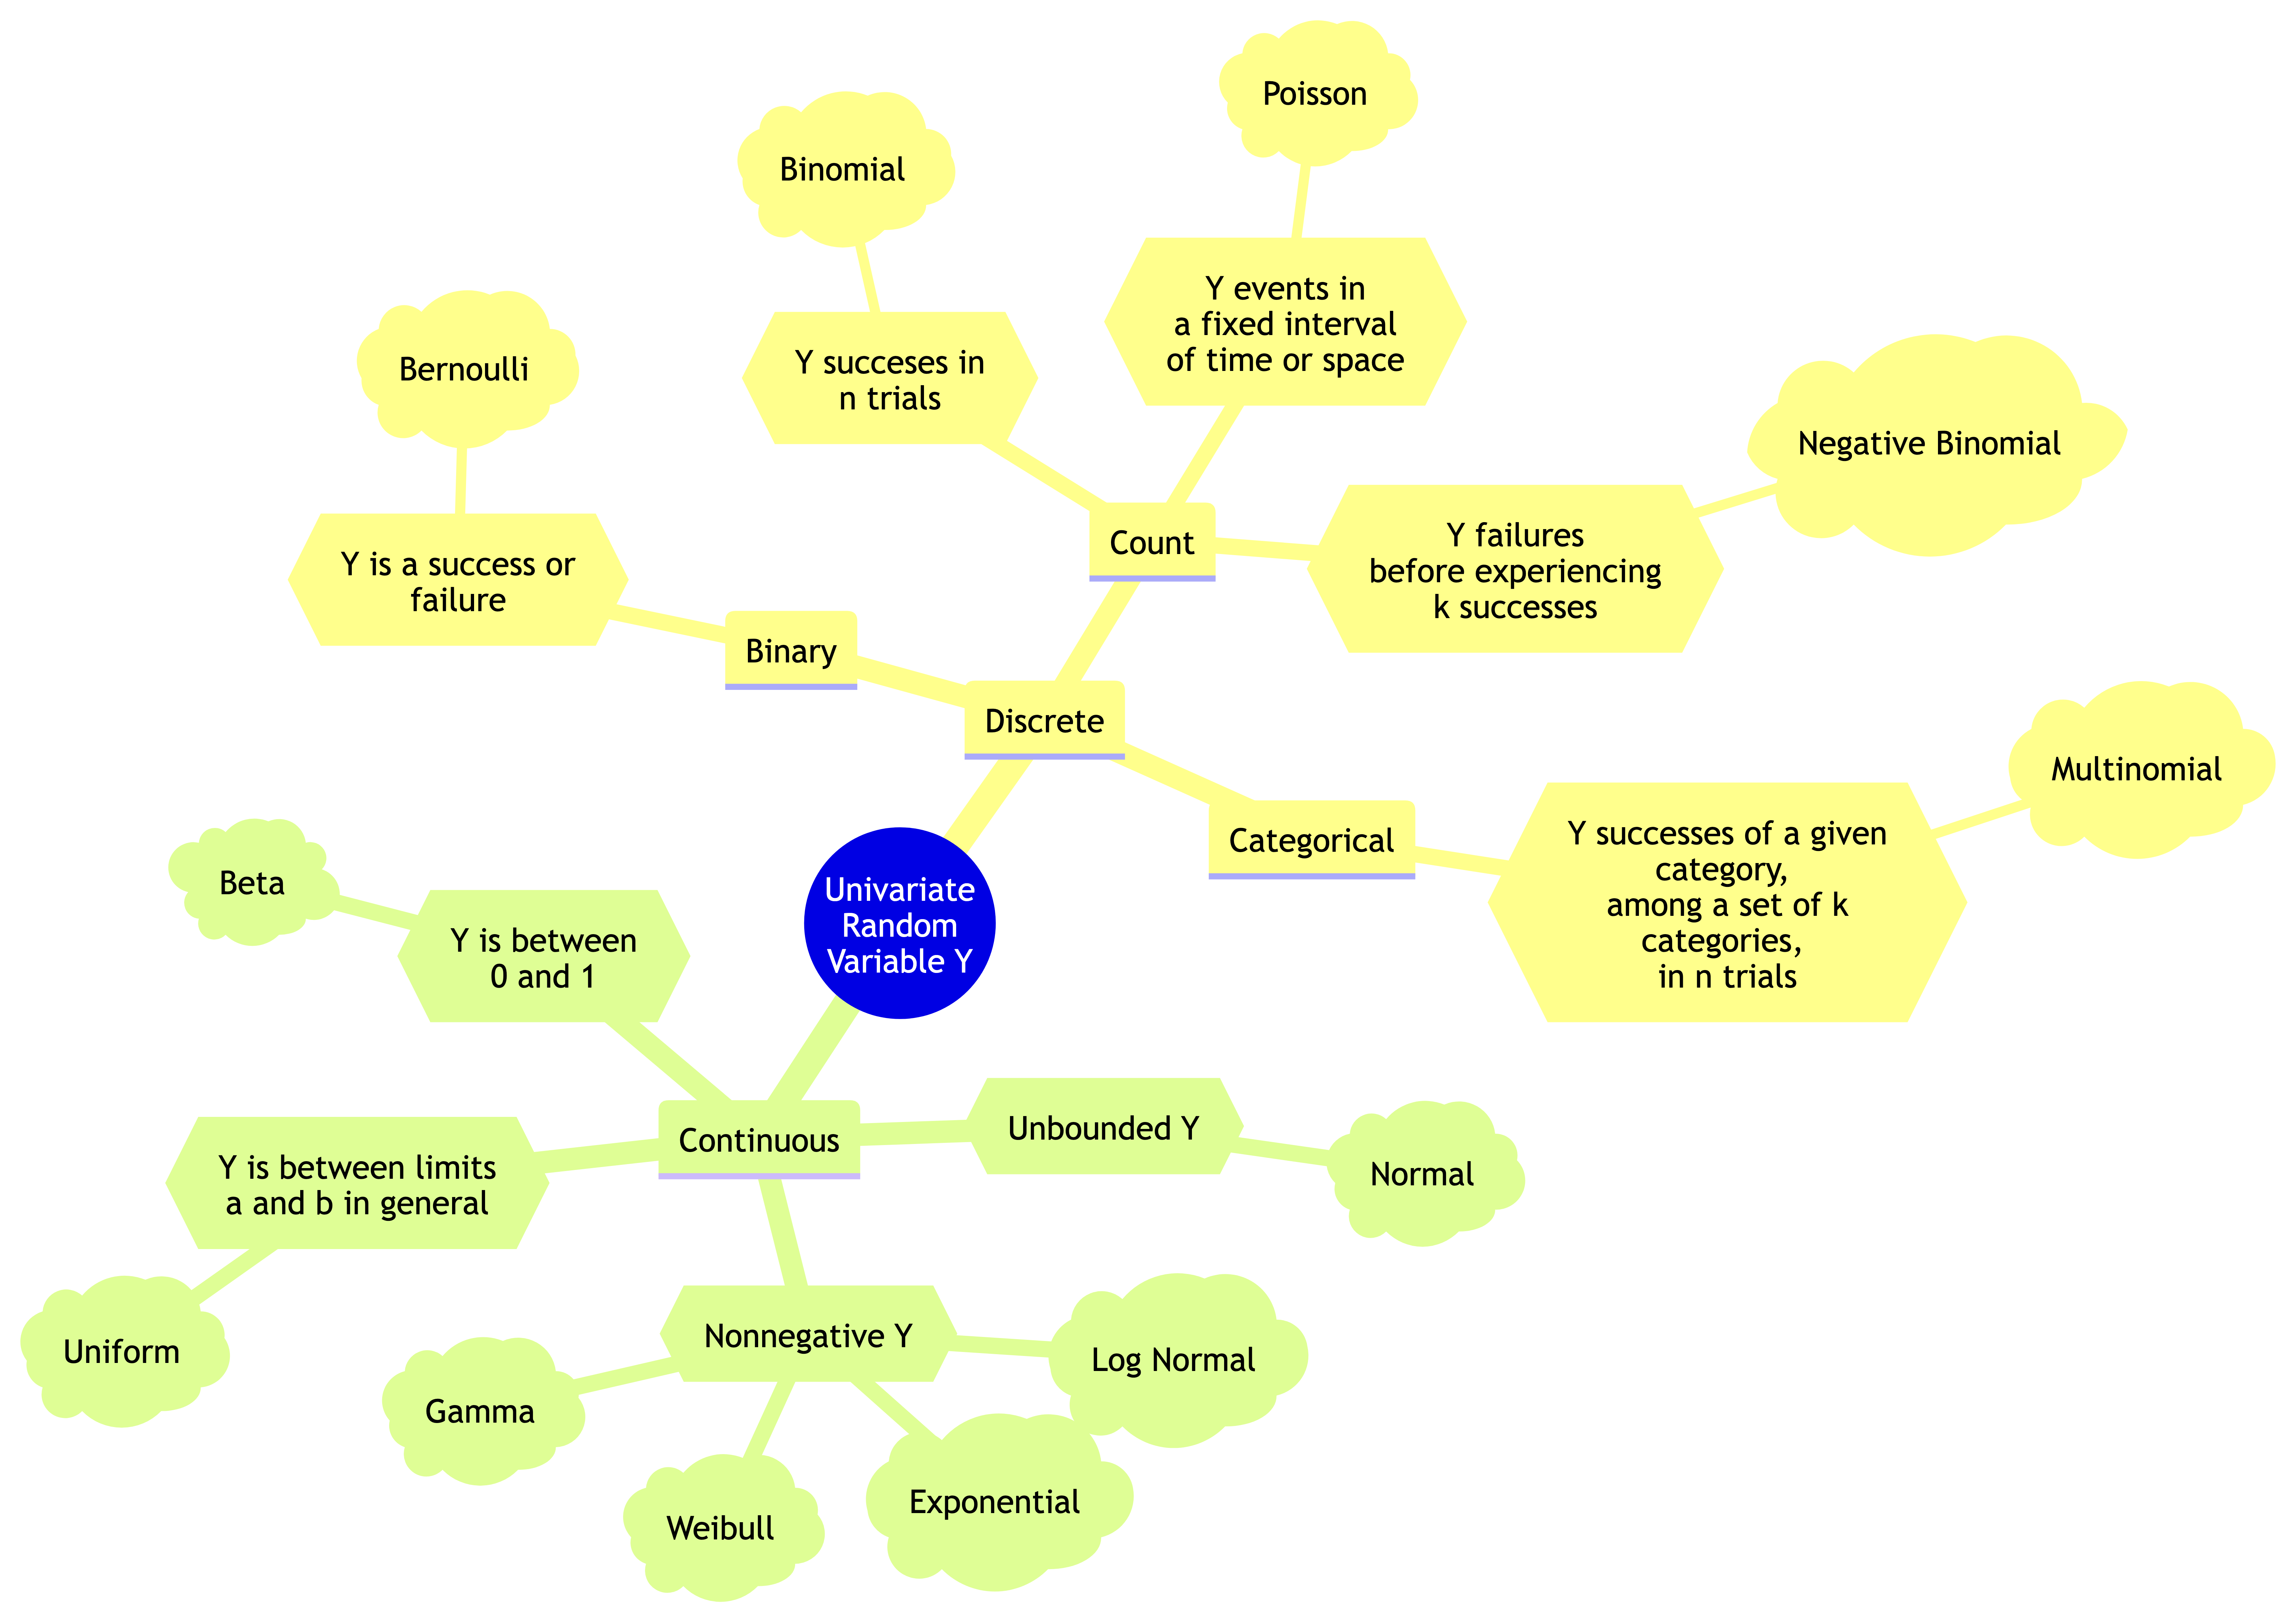
\includegraphics[width=11.75in,height=8.3in]{book/C-distributional-cheatsheet_files/figure-latex/mermaid-figure-1.png}




\end{document}
